\documentclass[11pt,a4paper]{ctexart}
%\usepackage{CJKutf8}
%\setCJKmainfont{AR PL UKai CN}
%\setCJKmainfont{AR PL UKai}
\usepackage{geometry}
\usepackage{caption}
\usepackage{graphicx, subfig,float}
\geometry{a4paper,left=4cm,right=4cm}
\usepackage{appendix}
\usepackage{amsmath}
\usepackage{enumerate}
\usepackage{amssymb,color}
\usepackage[colorlinks,linkcolor=red,anchorcolor=blue,citecolor=blue]{hyperref}
\usepackage{slashed}
\usepackage{simplewick}
\usepackage{tikz}
\usepackage{tcolorbox}
\usepackage[T1]{fontenc}
%colors
\def\blacktext#1{{\color{black}#1}}
\def\bluetext#1{{\color{blue}#1}}
\def\redtext#1{{\color{red}#1}}
\def\darkbluetext#1{{\color[rgb]{0,0.2,0.6}#1}}
\def\skybluetext#1{{\color[rgb]{0.2,0.7,1.}#1}}
\def\cyantext#1{{\color[rgb]{0.,0.5,0.5}#1}}
\def\greentext#1{{\color[rgb]{0,0.7,0.1}#1}}
\def\darkgray{\color[rgb]{0.2,0.2,0.2}}
\def\lightgray{\color[rgb]{0.6,0.6,0.6}}
\def\gray{\color[rgb]{0.4,0.4,0.4}}
\def\blue{\color{blue}}
\def\red{\color{red}}
\def\green{\color{green}}
\def\darkgreen{\color[rgb]{0,0.4,0.1}}
\def\darkblue{\color[rgb]{0,0.2,0.6}}
\def\skyblue{\color[rgb]{0.2,0.7,1.}}
%%control
\def\be{\begin{equation}}
\def\ee{\nonumber\end{equation}}
\def\beq{\begin{equation}}
\def\eeq{\end{equation}}
\def\bea{\begin{eqnarray}}
\def\eea{\end{eqnarray}}
\def\bmat#1{\left(\begin{array}{#1}}
\def\emat{\end{array}\right)}
\def\bcase#1{\left\{\begin{array}{#1}}
\def\ecase{\end{array}\right.}
\def\bmini#1{\begin{minipage}{#1\textwidth}}
\def\emini{\end{minipage}}
\def\tbox#1{\begin{tcolorbox}#1\end{tcolorbox}}
\def\pfrac#1#2#3{\left(\frac{\partial #1}{\partial #2}\right)_{#3}}
%%symbols
\def\bropt{\,(\ \ \ )}
\def\sone{$\star$}
\def\stwo{$\star\star$}
\def\sthree{$\star\star\star$}
\def\sfour{$\star\star\star\star$}
\def\sfive{$\star\star\star\star\star$}
\def\rint{{\int_\leftrightarrow}}
\def\roint{{\oint_\leftrightarrow}}
\def\stdHf{{\textit{\r H}_f}}
\def\deltaH{{\Delta \textit{\r H}}}
\def\ii{{\dot{\imath}}}
\def\skipline{{\vskip0.1in}}
\def\skiplines{{\vskip0.2in}}
\def\lagr{{\mathcal{L}}}
\def\hamil{{\mathcal{H}}}
\def\vecv{{\mathbf{v}}}
\def\vecx{{\mathbf{x}}}
\def\vecy{{\mathbf{y}}}
\def\veck{{\mathbf{k}}}
\def\vecp{{\mathbf{p}}}
\def\vecn{{\mathbf{n}}}
\def\vecA{{\mathbf{A}}}
\def\vecP{{\mathbf{P}}}
\def\vecsigma{{\mathbf{\sigma}}}
\def\hatJn{{\hat{J_\vecn}}}
\def\hatJx{{\hat{J_x}}}
\def\hatJy{{\hat{J_y}}}
\def\hatJz{{\hat{J_z}}}
\def\hatj#1{\hat{J_{#1}}}
\def\hatphi{{\hat{\phi}}}
\def\hatq{{\hat{q}}}
\def\hatpi{{\hat{\pi}}}
\def\vel{\upsilon}
\def\Dint{{\mathcal{D}}}
\def\adag{{\hat{a}^\dagger}}
\def\bdag{{\hat{b}^\dagger}}
\def\cdag{{\hat{c}^\dagger}}
\def\ddag{{\hat{d}^\dagger}}
\def\hata{{\hat{a}}}
\def\hatb{{\hat{b}}}
\def\hatc{{\hat{c}}}
\def\hatd{{\hat{d}}}
\def\hatN{{\hat{N}}}
\def\hatH{{\hat{H}}}
\def\hatp{{\hat{p}}}
\def\Fup{{F^{\mu\nu}}}
\def\Fdown{{F_{\mu\nu}}}
\def\newl{\nonumber \\}
\def\vece{\mathrm{e}}
\def\calM{{\mathcal{M}}}
\def\calT{{\mathcal{T}}}
\def\calR{{\mathcal{R}}}
\def\barpsi{\bar{\psi}}
\def\baru{\bar{u}}
\def\barv{\bar{\upsilon}}
\def\qeq{\stackrel{?}{=}}
\def\torder#1{\mathcal{T}\left(#1\right)}
\def\rorder#1{\mathcal{R}\left(#1\right)}
\def\contr#1#2{\contraction{}{#1}{}{#2}#1#2}
\def\trof#1{\mathrm{Tr}\left(#1\right)}
\def\trace{\mathrm{Tr}}
\def\comm#1{\ \ \ \left(\mathrm{used}\ #1\right)}
\def\tcomm#1{\ \ \ (\text{#1})}
\def\slp{\slashed{p}}
\def\slk{\slashed{k}}
\def\calp{{\mathfrak{p}}}
\def\veccalp{\mathbf{\mathfrak{p}}}
\def\Tthree{T_{\tiny \textcircled{3}}}
\def\pthree{p_{\tiny \textcircled{3}}}
\def\dbar{{\,\mathchar'26\mkern-12mu d}}
\def\erf{\mathrm{erf}}
\def\const{\mathrm{constant}}
\def\pheat{\pfrac p{\ln T}V}
\def\vheat{\pfrac V{\ln T}p}
%%units
\def\fdeg{{^\circ \mathrm{F}}}
\def\cdeg{^\circ \mathrm{C}}
\def\atm{\,\mathrm{atm}}
\def\angstrom{\,\text{\AA}}
\def\SIL{\,\mathrm{L}}
\def\SIT{\, \mathrm{T}}
\def\SIkm{\,\mathrm{km}}
\def\SIyr{\,\mathrm{yr}}
\def\SIGyr{\,\mathrm{Gyr}}
\def\SIV{\,\mathrm{V}}
\def\SImV{\,\mathrm{mV}}
\def\SIeV{\,\mathrm{eV}}
\def\SIkeV{\,\mathrm{keV}}
\def\SIMeV{\,\mathrm{MeV}}
\def\SIGeV{\,\mathrm{GeV}}
\def\SIcal{\,\mathrm{cal}}
\def\SIkcal{\,\mathrm{kcal}}
\def\SImol{\,\mathrm{mol}}
\def\SIN{\,\mathrm{N}}
\def\SIHz{\,\mathrm{Hz}}
\def\SIm{\,\mathrm{m}}
\def\SIcm{\,\mathrm{cm}}
\def\SIfm{\,\mathrm{fm}}
\def\SImm{\,\mathrm{mm}}
\def\SInm{\,\mathrm{nm}}
\def\SImum{\,\mathrm{\mu m}}
\def\SIJ{\,\mathrm{J}}
\def\SIW{\,\mathrm{W}}
\def\SIkJ{\,\mathrm{kJ}}
\def\SIs{\,\mathrm{s}}
\def\SImus{\,\mathrm{\mu s}}
\def\SIkg{\,\mathrm{kg}}
\def\SIg{\,\mathrm{g}}
\def\SIK{\,\mathrm{K}}
\def\SImmHg{\,\mathrm{mmHg}}
\def\SIPa{\,\mathrm{Pa}}
\def\rad{\,\mathrm{rad}}

\graphicspath{{figure/}}
\usepackage{enumerate}
%\usepackage{fancyhdr}
%\cpic{<尺寸>}{<文件名>}}用于生成居中的图片。
\newcommand{\cpic}[2]{
\begin{center}
\includegraphics[scale=#1]{#2}
\end{center}
}
%\cpicn{<尺寸>}{<文件名>}{<注释>}用于生成居中且带有注释的图片,其label为图片名。
\newcommand{\cpicn}[3]
{
\begin{figure}[H]
\cpic{#1}{#2}
\caption{\color{red}#3\label{#2}}
\end{figure}
}

\crefname{equation}{}{}
\crefname{figure}{图}{图}
\crefname{footnote}{注释}{注释}
\crefname{table}{表}{表}
\title{实验D1 锁相放大器与弱信号测量(必做)}
\begin{document}
\maketitle
\begin{tabular}{|p{8em}|p{8em}|p{8em}|p{5em}|}
\hline
		实验方案 &实验记录  &分析讨论 &总成绩\\
		\hline
		        &          &          &  \\
	    \hline
	\hline 
	年级、专业: &17级物理学 &组号:& 6 \\
	\hline
	姓名:& 徐昊霆 &学号:&17353071  \\
	\hline
	日期:& \today &教师签名: &  \\
    \hline	
        \end{tabular}

\begin{enumerate}
 \item 实验报告由三部分组成:
 \begin{enumerate}
  \item[1)]预习报告:(提前一周)认真研读\textbf{\uline{实验讲义}},弄清实验原理;实验所需的仪器设备、用具及其使用(强烈建议到实验室预习),完成讲义中的预习思考题;了解实验需要测量的物理量,并根据要求提前准备实验记录表格(由学生自己在实验前设计好,可以打印)。预习成绩低于50\%者不能做实验{\color{red} (实验D2和D3需要提前一周的周四完成预习报告交任课老师批改,批改通过后,才允许做实验)}。

  \item[2)]实验记录:认真、客观记录实验条件、实验过程中的现象以及数据。实验记录请用珠笔或者钢笔书写并签名({\color{red}用铅笔记录的被认为无效})。{\color{red}保持原始记录,包括写错删除部分,如因误记需要修改记录,必须按规范修改。}(不得输入电脑打印,但可扫描手记后打印扫描件);离开前请实验教师检查记录并签名。
  \item[3)]分析讨论:处理实验原始数据(学习仪器使用类型的实验除外),对数据的可靠性和合理性进行分析;按规范呈现数据和结果(图、表),包括数据、图表按顺序编号及其引用;分析物理现象(含回答实验思考题,写出问题思考过程,必要时按规范引用数据);最后得出结论。
 \end{enumerate}
 \textbf{实验报告}就是预习报告、实验记录、和数据处理与分析合起来,加上本页封面。
 \item 每次完成实验后的一周内交\textbf{实验报告}。
 \item 除实验记录外,实验报告其他部分建议双面打印。
\end{enumerate}
\newpage
\tableofcontents
\newpage
\section{实验原理与方案}
\subsection{实验目的}
\begin{enumerate}
 \item[1.]了解锁相放大器工作原理和特点,掌握锁相放大器基本参数含义及锁相放大器的基本 操作;复习示波器的使用;(实验内容 1)
  \item[2.]掌握用锁相放大器检测出湮没于噪声中的弱信号方法;(实验内容 2)
  \item[3.]通过本实验更加直观的了解方波的高频成分,并掌握用锁相放大器检测微弱信号中的谐波;(实验内容 3)
\item[4.]掌握交流四引线法精密测量小阻抗的原理和方法,理解相位的物理含义及电压与电流之间相位差的测量方法;(实验内容 4,探索)
\item[5.] 学习 VISA 接口协议,通过 LabVIEW 环境用 PC 机控制锁相放大器数据采集;(实验内容 4)
\item[6.]了解 PN 结结电容,探究变容二极管内 PN 结电容与反偏电压的关系;(实验内容 5)
\item[7.] 通过实验了解热噪声的特征,理解热噪声的本质及其统计意义。(实验内容 6,探索)
\end{enumerate}


\subsection{仪器用具}
\begin{table}[H]
\cpic{0.4}{t1}
\caption{弱信号检测实验仪器用具}
\end{table}

\subsection{实验安全注意事项}

1. OE1022 锁相放大器输入端不能接入强信号;接入信号需限定在 1V 以下。

2. OE4004 稳流源的电流输出不能直接接入 OE1022 锁相放大器的输入端。

\subsection{实验原理}
\subsubsection{噪声的定义及数学描述}
现代测量中,所有的物理最终都转换为电压或光强进行记录和处理,我们称之为携带被测量物理量信息的电或光信号;然而所有的测量,即使完全由机器自动进执行,结果都不可避免地引入待测量以外的其他信息,如环境干扰、不确定等,在所测量的信号不可避免地携带了噪声。测量结果(信号$x(t)$)可以视作被测量信号$s(t)$与噪声$n(t)$的叠加$x(t) = s(t) + n(t) $。
\par
一般来说,信号是运载信息的工具,是信息的载体。任何携带某个现象属性或行为信息的物理量都可以作为信号,如光信号、声信号和电信号等。物理世界中的信号都是有规律地随时间或空间变化的。数学上以函数的形式$x(t)$描述信号。
\par
最简单的信号用单一频率的三角函数的描述
\beq \label{eq1}
s_\omega (t) = a \cos (\omega_0 t + \varphi) 
\eeq
它包含了三个最基本的信息,即振幅$a$、频率$\omega_0$和相位$\varphi$,它对于信号载体对应着不同的物理含义。在实际应用中,人们往往只用到其中的一个或两个基本信息来进行信号传递或处理,而对于科学探索可能会全方位地用到所有的信息。\cref{eq1}是在时域下对信号的描述;在频域下该信号的数学描述为:
\beq
s_e(\omega) = \begin{cases}
a &, \omega = \omega_0 \\
0 &, \omega \not= \omega_0
\end{cases}
\eeq
其形式更简单,但丢失了相位的信息。基本信号的更一般数学描述是复数形式:
\beq
s_\omega (t) = ae^{i (\omega t + \phi)}
\eeq
它包含了式$\cref{eq1}$描述的实况和虚部,具有更丰富的物理内含和更简洁的数学表达。
\par
一般周期性的信号(函数)都可以傅立叶级数展开:
\beq \label{eq4}
s(t) = \sum_m a_m e^{i(m \omega_0 t + \varphi)}
\eeq
因此,只要讲清楚一种基本形式的信号处理过程,就可推广到一般的信号处理过程。
\par
广义地说,不是待测信号本身的、对测量值的贡献都可视为噪声。它可分为来自外界的环境噪声,最典型的是市电噪声($50\mathrm{Hz}$);以及来自被测量对象本身的噪声,如热噪声。它们都混合待测信号的测量值中。
\par
从物理角度来看,任何待物理量都包含无规、随机的变化,这就是噪声。它是对有规律的信号的一种随机干扰,往往被扩展为与待测信号相冲突的无用信号。例如白噪声,是电子器件和电路中常见的一种噪声,电阻的热噪声,PN结的散弹噪声等都是白噪声,它在时域和频域都呈均匀分布。换句话说,对于一项实验,噪声可来自于实验对象本身,也可来自于测量系统, 包括传感器和测量仪器,更可能来自于实验系统以外的环境。
\par
白噪声还有帮助人们缓解心情的功效(参见~\cite{white})。白噪音在哪方面可以发挥它的声音治疗功效呢?对于新生儿的父母来说,利用白噪音来停止婴儿的哭泣是一个很有效的声音治疗方法。例如,新生儿刚刚离开妈妈的子宫,来到一个陌生的环境,这对他们来说是需要一个适应过程的,而我们生活环境中一些陌生的声音对它们来说有时会另他们感到不安,以及烦躁。他们更喜欢子宫里的嘈杂声,而白噪音与他们熟悉的这种声音有着类似之处。因此,在很多孩子感到不安的时候,听到这种声音都会安静下来。特别是对那些患有新生儿疝气的孩子,他们经常会因为身体的不适以及对环境的不适应而莫名其妙的大声哭闹。一些经常受到环境噪音污染的人群会利用白噪音来帮助他们恢复工作效率,像一些大学生或办公室工作人员会利用白噪音来降低那些施工噪音对他们集中力产生的不良影响。白噪音甚至被公认为对于精神分散疾病、耳鸣、听觉过敏症以及多动症等神经系统疾病来说,是一种有效的“声音化妆处理”治疗。还有一些人利用白噪音来把一些可以打断他们正常睡眠的声音弱化。不仅是那些要在白天睡觉晚上工作的夜班族利用白噪音来削减白天有可能打扰到他们睡眠的一切声音。还有那些夜晚铁道附近的轰隆声,以及狗叫声,甚至你配偶的打鼾声等等都可以被白噪音的“屏蔽”功能所弱化。这样一来,你完全可以好好的睡上一觉,无论是处在怎样的一个睡眠环境。
\par
对于有规律变化的环境噪声,可用\cref{eq4}式来表述:它的频率可能与待测信号的频率相同或相近,但更可能是其他频率。在时域可以看成频率不同、振幅随机的“信号”叠加(讲义~\cite{lec}中这里似乎有错误)
\beq
n(t) = \sum_\omega b(\omega) e^{i\omega t}
\eeq
其中振幅$b(\omega)$可能是常量(如市频干扰),亦可能是随机量$r(\omega)$;在频域中,随机噪声也可以理解为每一时刻的噪声电压频谱$n(\omega) $都不会是一样的\footnote{拟有误,随机噪声应该理解成一维随机高斯场。}

信噪比是科学与工程中所用的一种度量,用于比较所需信号的强度与背景噪声的强度,表 征噪声对信号的覆盖程度。
通过信号处理可提高信噪比,即提高了信号质量。为反映信号质量改善的程度,定义信噪改善比$SNIR$。
\beq
SNIR = \frac{SNR_0}{SNR_i}
\eeq
式中,$SNR_o$是经过处理(系统输出端)的信噪比,$SNR_i$是未经过处理(系统输入端)的信噪 比。$SNIR$越大,表明系统抑制噪声的能力越强。
\par
“微弱信号”不只意味着信号的绝对幅度很小,而是相对于噪声而言幅度很小,特别是那些被噪声淹没的信号,都称作微弱信号。只有在有效地抑制噪声的条件下放大微弱信号的幅度, 才能提取出真实的信号。因此,微弱信号检测所一门专门针对噪声的技术,其主要任务是提高信噪比。\par
提高信噪比的途径有两方面:一是通过物理屏蔽来抑制环境噪声,还可以通过不做实验来避免遭遇噪声,另一方面是通过信号处理滤除噪声。通常物理屏蔽的代价不少,关键是有另一类噪声在理论上不能通过物理屏蔽来抑制或隔断,它就是来自测量对象本身的噪声,尽管此类噪声在幅度上可能远低于环境噪声;因此,对于不能被屏蔽的噪声,信号处理就成为唯一的选择。\par
为了从噪声中提取出有用的信号,就需要研究噪声的来源与性质,分析噪声产生的原因和规律,以及噪声的传播途径,有针对性地采取有效措施抑制噪声,研究被测信号和噪声的统计特性及其差别,以寻找出从背景噪声中检测出有用信号的方法。
\subsubsection{滤波法}
\par
小信号是相对微弱信号信噪比更高的信号,可以采用{\bf 滤波}的方法进行信噪比的提升以实现精确测量。
\par
设输入信号为$s(t) + n(t)=a \cos(\omega_0 t+\varphi)+\sum_{-\infty}^{\infty}b(t,\omega)\cos(\omega t)$。带通滤波的作用是删去$(\omega_0 - \frac{\Delta \omega}{2} , \omega_0+ \frac{\Delta \omega}{2})$以外的信号,滤波后的总信号为
\beq
a \cos(\omega_0 t) +\sum_{\omega_0 -\Delta \omega/2}^{\omega_0 + \Delta\omega/2}b(t,\omega)\cos(\omega t)
\eeq
还可以使用低通滤波的方法,低通滤波的方法即设定一个截止频率,删去高频的部分,滤波之后信号为
\beq
A a\cos(\omega_0)t+ A\sum_0^{\omega_{\rm cut-off}}b(t,\omega)\cos(\omega t) = a\cos(\omega_0 t)+ n_l(t)
\eeq
其中$A$为放大倍数。可见,滤波后带通外的噪声仅在一个带通内表达(仅由式(D1-9)或(D1-
10)的右边第二项描述),从时域看噪声水平明显下降,信噪比得到明显改善。但带通内的噪声
不能被滤掉,且与信号一起同时被放大,我们称这部分噪声为同频噪声。
\par
实际中可以用示波器进行简单滤波,如\cref{filter}。
\cpicn{0.6}{filter}{$Q$值为 20 的滤波器滤波前后的信号:(a)、(b)分别为滤波前后的时域图;(c)、(d)分别为滤波前后的频域图。}
\subsubsection{零位法}
\par
\cpicn{0.5}{d16}{零位法原理示意图}
另一种削弱噪声信号的方法为{\bf 零位法}(null method),零位法的本质是比较法测量。一般直接指示型测量仪表的测量方法是将被测信号放大到一定幅度,以驱动表头指针的偏转角度指示被测量的大小;或者经模数转换和数据处理后由液晶显示被测量的数值。而零位法是调整对比量的大小使其尽量接近被测量,由对比量指示被测量的大小,如\cref{d16}所示。图中的零位表指针只用来指示被测量和对比量的差异值,当零位表指示近似为零时,对比量的大小就表征了被测量的大小。对比量的调整可以手动实现,也可闭 环自动调整,如\cref{d16}中虚线所示。用这种方法测量的分辨率取决于对比量的调整和指示的分辨率。用机械测量类比,弹簧秤是一种直接指示仪表,而天平则是一种零位法仪表。
\par
由\cref{d16}可以看出,虽然被测量和对比量在传输过程中分别附加了干扰噪声$n_1(t)$和$n_2(t)$,但是在对比相减的过程中,$n_1(t)$和$n_2(t)$会在一定程度上相互抵消。两路信号传输过程越相似,$n_1(t)$和$n_2(t)$也会越近似,抵消作用越好。因此,与直接指示测量方法相比,零位法测量结果的信噪比更高,测量精度也更高。
\par
设被测信号
\beq
x(t) = s(t) + n_1 (t)
\eeq
对比量信号
\beq
x_r(t) = s_r(t) + n_2 (t)
\eeq
测量其差值得到
\beq
\Delta x (t) = s(t) - s_r(t) + n_1(t) - n_2(t)
\eeq
当调节对比量使得零位表计数为零时,$\Delta x = 0$,则$s(t) = n_1(t)-n_2(t)$,两组噪声相互抵消,则
\beq
s(t) \simeq s_r(t)
\eeq
可见,零位法更适合于抑制同源噪声(如环境噪声),但不适用于随机的热噪声。
\subsubsection{锁相放大法}
\par
锁相放大器(lock-in amplifier, LIA)也称锁定放大器,是通过特定的载波将湮没在噪声中的微弱信号提取出来的技术。锁相放大技术采用了频谱迁移和交流放大技术、用相敏检测器和低通滤波器来实现调制信号的解调。锁相放大器抑制噪声有三个基本出发点:
\begin{itemize}
\item 用调制器将直流或慢变信号的频谱\footnote{讲义此处有错字}迁移到调制频率$\omega_0$处,再进行放大,以避开传输过程所引入的以及放大器内部的$\frac{1}{f}$噪声的不利影响。
\item 利用相敏检测器实现被调制信号的解调过程,可以同时利用频率$\omega_0$和相角$\theta$进行检测,噪声与信号同頻又同相的概率很低。
\item 用低通滤波器来抑制宽带噪声。电路实现时,低通滤波器的频带可以做得很窄,而且 其频带宽度不受调制频率的影响。
\end{itemize}
锁相放大技术需要先对(慢变)信号频谱进行迁移,如\cref{d17},其调制过程是将低 频信号$V$乘以频率为$\omega_0$的正弦载波,从而将其频谱迁移到调制频率$\omega_0$的附近,之后进行选频放大,这样就不会把$\frac{1}{f}$噪声和低频漂移也放大了,如\cref{d17}(a)所 示,图中的虚线表示$\frac{1}{f}$噪声和白噪声的功率谱密度。经交流放大后,再用相敏检测器将其频谱迁移到直流($\omega = 0$)的两边,用窄带低通滤波器滤除噪声,就得到高信噪比的放大信号,如\cref{d17}(b)所示,图中用虚线表示低通滤波(LPF)的频率响应曲线。只要 LPF 的带宽足够窄,就能有效地改善信噪比。
\cpicn{0.6}{d17}{锁相放大器对信号频谱进行迁移的过程}
通过锁相放大技术的过程,相当于一个$Q$值极高的窄带滤波器,可以不受待测频率以外的噪声信号影响,从而使检测系统的性能大为改善。锁相放大器的等效噪声带宽可以达到$0.0001\mathrm{Hz}$,整体增益可以高达 1010 以上,即把$0.1\mathrm{nV}$的微弱信号可以放大到$1.0\mathrm{V}$以上,因而可以测量极其微小的信号。
\subsubsection{工作原理}
锁相放大器的基本结构如\cref{d19}所示的虚线框内,其中信号通道、参考通道为锁相放大器的输入通道,相敏检测器(PSD)和低通滤波器(LPF)等。对于三角函数信号,可直接从信号通道输入(虚线框内的)锁相放大器。对于非三角函数信号或慢信号(如直流信号),它在输入锁相放大器前,需要被与参考信号频率相同的信号所调制(如\cref{d19}虚线框外部分所示),参考信号既可以是外部输入,也可以是内部自带参考信号源提供。为不失一般性,以下数学推导以需要调制的非三角函数信号为出发点。
\cpicn{0.4}{d19}{锁相放大器工作原理(虚线框内)}
\par
设带噪声的待测信号
\beq
f(t)= s(t) + n(t)
\eeq
调制并放大$A_I$倍后的信号为
\beq
u(t) = A_I f(t) \sin \left(\omega_{0} t+\theta\right) = A_I s(t) \sin \left(\omega_{0} t+\theta\right) + A_I n(t) e\sin \left(\omega_{0} t+\theta\right)
\eeq
此时,信号与噪声都被同时放大了。
\par
锁相放大器采用参考信号$u_{r}(t)=\sin \left(\omega_{0} t\right)$解调,因调制信号是用参考信号通过某种物理机制触发或用参考信号本身,因此,参考信号与调制信号频率相同、相位差确定。
\bea
u_{p}(t)&=u_{r}(t) u_{\mathrm{s}}(t)=A_{I}[s(t)+n(t)] \sin \left(\omega_{0} t+\theta\right) \sin \left(\omega_{0} t\right) \\ &=\frac{1}{2} A_{I}[s(t)+n(t)]\left[\cos \theta-\cos \left(2 \omega_{0} t+\theta\right)\right]
\eea
低通滤波后留下了慢变的待测信号和同(低)频噪声:
\beq
u_{ox}(t)=\frac{1}{2} A_{I}\left[s(t)+n_{l}(t)\right] \cos \theta
\eeq
另一路相位相处$\frac{\pi}{2}$的信号经相同处理后得到
\beq
u_{o y}(t)=\frac{1}{2} A_{I}\left[s(t)+n_{l}(t)\right] \sin \theta
\eeq
于是被调制后信号(锁相放大器输入端信号)相对于解调信号的相位差
\beq
\theta=\arctan\frac{u_{o y}(t)}{u_{o x}(t)}
\eeq
输出信号振幅
\beq
u_{o}(t)=\sqrt{u_{\mathrm{ox}}^{2}(t)+u_{\mathrm{ov}}^{2}(t)}=\frac{1}{2} A_{I}\left[s(t)+n_{l}(t)\right]
\eeq
具有这种两互相垂直的信号输出、获得锁相放大器输入端完整信号能力的锁相放大器被称双相锁相放大器,本实验用的OE1022就是双相锁相放大器。信号的有效值
\beq
R=\sqrt{\frac{\sum_{0}^{N_{r}}\left\{\left[\left(s\left(t_{i}\right)+n\left(t_{i}\right)\right) \cos \left(\omega_{0} t\right)\right]^{2}+\left[(s(t)+n(t)) \sin \left(\omega_{0} t\right)\right]^{2}\right\}}{N_{T}}} \approx \frac{u_{o_{0} p p}(t)}{\sqrt{2} A_{t}}
\eeq
则锁相放大器输入信号的$x$、$y$分量分别为:
\bea \label{measure}
X&=R \cos \theta \approx \frac{u_{o x_{-} p p}(t)}{\sqrt{2} A_{I}} \\
Y&=R \sin \theta \approx \frac{u_{o y_{-p p}}(t)}{\sqrt{2} A_{I}}\\
R&=\sqrt{X^{2}+Y^{2}}
\eea
其中$R$、$X$、$Y$和$\theta$就是在锁相放大器屏幕上的显示值,是内部运算的结果;当噪声足够小、且$s(t)$为常量时,$R$为一常量。
\par
可见,锁相放大器用相敏检测器实现解调,并且实现既检幅又检相的功能。尽管锁相放大器已滤除了绝大部分噪声,但对同频噪声$n_l (t)$仍无能为力。并且由于放大后的信号仍包含噪声成分,等效于其相位差$\theta$也受随机噪声$n_l (t)$影响,从而存在相位噪声。在实际工作中,我们通常选择频谱中背景噪声最低的频率作为慢变信号的调制频率。\par
很多应用场合,锁相放大器的参考信号由外部提供(例如光学斩波器,信号发生器),此时叫做外部参考模式。锁相放大器的参考通道就会将外部输入的参考信号进行放大和整形,然后通过锁相环技术,在锁相放大器内部产生一个与外部输入参考信号频率相等、相位差锁定的的正弦信号。可见,锁相的含义是根据外部参考,利用锁相环产生一个频率相同、相位差锁定的参考信号。这个是锁相放大器能够进行后面相敏检测运算的基础。参考通道还有另一功能,即对参考输入进行移相处理,以使各种不同相移信号的检测结果达到最佳。
\par
如果采用内部参考模式,也就是锁相放大器自带的 SINE OUT 的正弦信号作为实 验的激励源,由于内部参考信号是锁相放大器自身产生的正弦波(与 SINE OUT 信号同频不同 相),因此频率及相位不需要锁相环获取,此时也就不用锁相;在这种情况下,由于频率及相 位是直接得到的,不需要放大和整形,测量的精度会更高。
\par

对于数字锁相放大器 Output 通道的输出信号,对应于原信号$R$或$X$、$Y$分量乘以其逻辑增益。电路实现时,LPF 的频带可以做得很窄,使锁相放大器达到较大的 SNIR。
\par
锁相放大器有几个重要参数:灵敏度,最小可测信号 MDS,时间常数,陡降,满刻度输出时的输入电平 FS,过载电平 OVL,输入总动态范围,输出动态范围,动态储备 DR,选频放大。锁相放大器的重要参数,影响着锁相放大器的工作。理解锁相放大器参数的含义及其(配置)对锁相放大器性能的影响,是正确使用锁相放大器的前提。
\begin{enumerate} 
\item 灵敏度从直观上来分析就是锁相放大器的当前显示量程,由信号通道的交流放大增益与相敏检波器解调增益决定。
\item 最小可测信号定义为输出能辨识的最小输入信号,可以理解为系统对小信号的分辨率。影响 MDS 的主
要因素有系统的内部噪声、温度漂移等,即结果会受到包括内部噪声、温度漂移的影响而产
生波动,MDS 定义为输出可以稳定在一定百分率波动下的最小输入。
\item 时间常数是低通滤波器$RC$电路的时间常数。可以简单地认为,时间常数越大,阶数越高,输出的带宽就越低,显示的测量幅度、相位等值就越稳定。然而,过大的时间常数会抹平输入信号(随时间)的变化,从而失去有用的信息。因此,在实际应用中,需要根据输入信号随时间变化的情况,协调时间常数与信噪比之间的平衡。
\item  FS 有时也称为满刻度灵敏度,它是用来表征锁相放大器测量灵敏 度的,拥有电压的量纲,与系统的总增益有关。
\item OVL 定义为锁相放大器任一级出现过载或临界过载时的输入电平。因为微弱信号检测通
常处理的是信噪比较低的输入,所以过载往往出现在噪声电压出现尖峰时。因此,可以将
OVL 理解为系统允许的最大输入噪声电压电平,即系统的最大噪声容限。应当指出,通常对
应不同的增益设置,各级放大情况将有所不同,其过载电平也会有所不同,故在指明 OVL
时,应当附带指出其 FS,这样才有意义。
\item  在给定 FS 的条件下(即给定的增益设置),锁相放大器的过载电平 OVL 与最小可测信
 号 MDS 比值的分贝数
 \beq
\text{输入总动态范围} = 20 \mathrm{lg\ } \frac{OVL}{MDS} \mathrm{dB}
\eeq
上文已经介绍,OVL 标称了锁相放大器的噪声容限,而 MDS 表明锁相放大器能够分辨的
最小信号。因而输入总动态范围可以理解为锁相放大器从噪声中提取有用信号的能力,即分
辨率越高,噪声容限越大,则输入总动态范围越大。
 \item 该参数定义为满刻度灵敏度 FS 与最小可测信号 MDS 比值的分贝数,即
 \beq
 \text{输出动态范围} = 20 \mathrm{lg\ } \frac{FS}{MDS} \mathrm{dB}
\eeq
 输出动态范围表示锁相放大器可以检测的有用输入信号的动态范围,即输入有效信号可以在该范围内波动而既不会导致锁相放大器不可分辨,也不会导致超过输出的最大范围。
 \item 动态储备 DR 定义为过载电平 OVL 与满刻度输出时的输入电平 FS 比值的分贝数
 \beq
 DR = 20 \mathrm{lg\ } \frac{OVL}{FS} \mathrm{dB}
\eeq
\par
锁相放大器输入信号在 PSD 处理之前需要交流放大,而在 PSD 处理之后是直流放大信号即可。在总增益不变的情况下,如果调整交流增益增加,直流增益减小,则输入噪声经交流放大很容易使 PSD 过载,动态储备减小,同时输出的直流漂移减小。反之,如果增加直流增益,降低交流增益,则动态储备提高,使锁相放大器具有良好的抗干扰能力,但以输出稳定性为代价,降低了测量精度。\par
在确定的测量精度要求下,动态储备有最小值。精度要求越高,其最小值就越大。在模拟锁相放大器中,低动态储备意味着更小的输出误差和漂移。在 OE1022 数字锁放中,高动态储备不会增加输出误差和漂移,但是会增加输出噪声。然而,如果在 A/D 转换器前的模拟放大器增益足够大,则其被放大的自身噪声比 A/D 转换器的噪声还大。这样,输出主要受输入噪声影响。因此,增大模拟增益即减小动态储备并不能减小输出噪声。在分辨率要求极高的情况下,增益增大并不能提高信噪比,因此,这时可以降低增益从而提高动态储备。
\item 
 选频放大对某一段频率或单一频率的信号具有突出的放大作用,而对其他频率的信号具有较强抑制作用的放大。
 \end{enumerate}
\subsection{实验前思考题}
\subsubsection{实验一}
1. 请写出拍频信号的数学表达式,并分别用时域和频域图表述出来。

拍频信号的本质就是两个频率相近的信号的叠加,为了突出原理起见,我们假设两个信号振幅相同。设两个信号分别为
\bea
E_1 &=& E_0 \cos(\omega_1 t +\varphi_1) \\
E_2 &=& E_0 \cos(\omega_2 t +\varphi_2)
\eea
通过三角函数公式
\beq
\cos \alpha + \cos\beta = 2\cos\left(\frac{\alpha + \beta}{2}\right)\cos\left(\frac{\alpha - \beta}{2}\right)
\eeq
我们得到两列信号的叠加为
\beq\label{pai}
E = E_1 + E_2 = E_0 \cos(\omega t +\varphi_0 )\cos(\Delta \omega t/2+ \Delta \varphi/2)
\eeq
在上式中,我们定义了
\bea
\omega &=& \frac{\omega_1+\omega_2}{2}\\
\Delta \omega &=& \omega_1 - \omega_2 \\
\Delta \varphi &=& \varphi_2 - \varphi_1\\
\varphi_0 &=& \frac{\varphi_1 - \varphi_2}{2}
\eea
将上述信号做傅里叶变换即可得到频域图,利用公式
\beq
\int e^{i\omega t}e^{-i\omega^{\prime}t} dt = 2\pi \delta(\omega - \omega^{\prime})
\eeq
我们得到三角函数的傅里叶变换
\bea
c(\omega) &=& \int cos(\Omega t)e^{i\omega t} dt \\
&=& \int \frac{e^{i \Omega t}+e^{-i\Omega t}}{2} e^{i\omega t} \\
&=& 2\pi \frac{\delta(\Omega - \omega)+\delta(\omega+\Omega)}{2}
\eea
\cpicn{0.5}{pai1}{拍频时域图}
\cpicn{0.5}{pai2}{拍频频域图}
从式~\ref{pai}中我们可以看出,叠加后的信号一方面在做快速振动,快速震荡的角频率为$\omega$,另一方面快速振动的振幅又在做相对来说较慢的振动,这种现象成为拍。假设两个频率相近的信号,将他们相加后画出的图像如~\cref{pai1}所示,将得到的图像做傅里叶变换,得到~\cref{pai2}。如~\cref{pai1},\cref{pai2}所示,我们确实可以看到叠加后的信号在做快速振动,将其做傅里叶变换到频域图中,发现两个信号的频率确实相近(相差远远小于他们的本身值。)

上面讨论仅仅是两列波实现的拍频现象,实际上,真正的信号由很多频率的三角函数叠加,如果这些信号的频率相近,也会得到上述拍频现象。

2. 噪声电压信号是个随机值,原则上,只要时间足够长,其平均值为零。如果待测信号是个恒定值,且环境噪声也是稳定的,则可以通过大量采样平均来获得待测信号值。
然而,实际测量中,信号不是常量,而是(相对)慢变量,而(环境)噪声也不稳定,
这样长时间大量采样平均的方法就不奏效,锁相放大器是个更好的解决方案。为更好
的使用锁相放大器,请回答以下问题:
1)如何用锁相放大器检测到待测的直流信号或慢变信号?(图 D1-9 中的 x(t)为直流
或慢变信号)
2)如用斩波器调制直流信号(如光强)
,被斩制后的信号(图 D1-9 中的$u_m(t)$ 信号)
仍然包含有直流分量(即平均值不为零),但该直流分量随交流信号输入锁相放
大器后不会被锁相放大器检测,请从数学推导上说明。
【注,一个理想的交流信号其平均值为零;一个平均值不为零的信号,其平均值可视为直
  流信号。】

1)检测到待测信号的手段有两个:
对于直流信号或慢变信号在输入到锁相放大器之前,待测信号会被与参考信号频率相同的信号调制,其频谱会迁移到调制频率附近,以避免放大器1/f噪声的影响,但待测信号仍然很弱,此时输入锁相放大器后会被放大器放大,以达到锁相放大器的最小可测信号的强度要求,接着输入相敏检测单元进行解调;解调信号由参考信号产生,与放大后的待测信号频率相同,相位差确定,对待测信号解调后再通过LPF,滤除宽带噪声,最后输出高信噪比的信号,也即检测到待测的直流信号或慢变信号。
2) 如果$u_m$仍然有直流分量$u_0$,设$u_m(t) = u_0+ x(t)\sin(\omega_0 t+ \theta)$,经过相敏检波器解调,假设解调信号为$A\sin(\omega_0 t)$,解调之后的信号为
\bea
u_p(t) &=& Ax(t) \sin(\omega_0 t +\theta)\sin(\omega_0 t)+A\sin(\omega_0 t)\\
&=& \frac{1}{2}(\cos \theta  - \cos(2\omega_0 t+\theta)) +Au_0 \sin(\omega_0 t)
\eea
解调后的信号会经过低通滤波器,大于频率阈值$\omega_{\rm cut-off}$的噪声会被除去,因此$u_p(t)$中频率为$2\omega_0,\omega_0$的噪声会被除去,不会对最终测得的相位差以及幅度等参量产生影响。



3. 相位角以及相位差的含义是什么?锁相放大器输出的是待测信号的相位角还是待测
信号与参考信号之间的相位差?

如果某一物理量随时间(空间)做正弦变化或余弦变化,决定该物理量在某一时刻相位角是在某一特定时刻(位置)决定信号状态的一个数值,即为相位角;以正弦波为例(实际上,任何一个信号都可以分解成很多三角函数的叠加)
\beq
x(t) = x_0 \cos(\omega t+\varphi)
\eeq
这里$\omega t +\varphi$就被称作相位
在$t=0$ 时的数值也被称为初相位角,这里的初始相位角是$\varphi$
考察频率相同的两个物理量,则二者之间相位差是二者的相位角的差。以时域
中的物理量为例,设二者角频率为$\omega$,
\bea
u_1 &=& A_1 \sin(\omega t +\varphi_1)\\
u_2 &=& A_2 \sin(\omega t +\varphi_2)
\eea
则两个信号的相位差为
\beq
\Delta \varphi = \varphi_2 - \varphi_1 +\omega \Delta t
\eeq
如果两个物理量所处的时刻相同,相位差就等于初始相位角的差,相位角收到时间、角频率、初始相位差的影响。

实际上,在测量中,只能测量到实际待测信号与参考信号的相位差,绝对的相位没有意义(因为相位的零点可以任意选取)。在本实验中,锁相放大器输出的是待测信号与参考信号的相位差,它收到调制信号与解调信号相位差的影响。


4. 请预测一根长 1.0 米的同轴电缆会给相位差的测量带来多大的影响?实验能测出来吗?多高的频率才能测出来?

我们要清楚,这里的相位差指的是调制后的信号与解调信号的相位差,而解调信号一般是由输入的信号通过某种物理机制产生的。因此,由于电缆的存在,信号在电缆中传播会引起额外的相位差,这一部分的相位差贡献到了调制后的信号的相位中,因此产生了相位差。根据介质中的麦克斯韦方程组(例如,参见~\cite{electromagnetic})
\bea
\nabla \cdot \vec{E} &=& \rho/\epsilon \\
\nabla \times \vec{E} &=& -\frac{\partial \vec{B}}{\partial t} \\
\nabla \cdot \vec{B} &=& 0\\
\nabla \times \vec{B} &=& \mu\vec{j} + \mu\epsilon \frac{\partial E}{\partial t}
\eea
利用公式
\beq
\nabla\times( \nabla\times \vec{E} ) =  \nabla(\nabla \cdot \vec{E}) - \nabla^2 \vec{E}
\eeq
将麦克斯韦方程组带入上式两边,利用欧姆定律,并取$\rho = 0 $,得到
\beq
\frac{\partial^2 \vec{E} }{\partial t^2}+\mu \sigma \partial_t \vec{E} - \frac{1}{\mu\epsilon} \nabla^2 \vec{E} =0
\eeq
上式实际上是一个波动方程,$\mu \sigma \partial_t \vec{E}$可以看做阻尼项,如果$\sigma$很小,则阻尼很小,实际上阻尼意味着一个弛豫时间,如果知道输入信号的强度和锁相放大器接受的信号强度,可以测量这个弛豫时间,进而测量金属电导率。所以我们得到,电磁场在电缆中传播的速度为
\beq
v = \frac{1}{\mu \epsilon} \simeq 10^8 \,\mathrm{m/s}
\eeq
因为电缆有$1$m长,所以在电缆的传播过程导致了时间差
\beq
\Delta t = \frac{l}{v}
\eeq
进而造成了相位改变
\beq\label{phase}
\omega \Delta t = 2\pi \nu \Delta t  
\eeq
所以当相位改变大于相位分辨率时,就能测出由上述效应导致的相位差变化。实验中用到的锁相放大器分辨率约为$0.01^{\circ}$,由上面的条件计算得到,信号的频率要大于$3\mathrm{kHz}$才能测出相位差。

6.(选)用复数取代三角函数,将锁相放大器的工作过程描述一遍;

设带噪声的待测信号
\beq
f(t)= s(t) + n(t)
\eeq
由于一般的信号都可以分解为频率不同的三角函数叠加,例如对于$f(t)$
\beq
f(t) = \sum_{n=0} a_n \sin(\omega_n t) +b_n \cos(\omega_n t) 
\eeq
现在将信号$f(t)$使用复数来表述,新的表示$\widetilde{f(t)}$记作
\beq
\widetilde{f(t)} = \sum_{n = -N} c_n e^{i\omega_n t}
\eeq
注意在复数表示下,$n$可以从负数开始。一般地,$c_n$是一个虚数。新的表示$\widetilde{f(t)}$与原来的表示关系为
\bea
c_n &=& \frac{a_n}{2i}+\frac{b_n}{2} \\
c_{-n} &=& -\frac{a_n}{2i} + \frac{b_n}{2}
\eea
为了验证这一关系,可以将此关系带入到新的表示的表达式中,化简就可以得到原来三角函数表示的形式。由上面的表示,显然有
\beq \label{eq:relation}
c_{-n} = c_{n}^{\dagger}
\eeq
这一关系保证了新的表示$\widetilde{f(t)}$是实数。

使用内部参考信号源(当信号来源于锁相放大器外)或是输入信号本身(当信号来源于锁相放大器内)调制并放大,得到的信号为
\beq
u(t) = A_I f(t) e^{i(\omega_0 t + \theta)}
\eeq
此时,信号与噪声都被同时放大了。
\par
锁相放大器采用参考信号$u_{r}(t)=e^{i \left(\omega_{0} t\right)}$解调,因调制信号是用参考信号通过某种物理机制触发或用参考信号本身,因此,参考信号与调制信号频率相同、相位差确定。
\bea\label{signal}
u_{p}(t)=u_{r}(t) u_{\mathrm{s}}(t) &=&\frac{1}{2} A_I [s(t)+n(t)] e^{i(2\omega_0 t+\theta)}
\eea
低通滤波后留下了慢变的待测信号和同(低)频噪声:
\beq
u(t) = \frac{1}{2} A_I [s(t)+n(t)] e^{i\theta}
\eeq
上面信号的模长为$ \frac{1}{2} A_I [s(t)+n(t)]$,幅角为$\theta$。由前面的关系~\cref{eq:relation}可以知道,对于$-n$项,信号实际上是复数表示的虚部,而对于$n$项,信号是复数表示的实数部分。现在,对于不同的$n$,考虑到低通滤波并求所有信号的有效值,得到
\beq
R = \sqrt{\frac{ \sum_{-N_r}^{N_r}\left[\mathrm{Re}u_i(t)+\mathrm{Im}u_i(t)\right]^2}{N_T}}
\eeq
当噪声足够小时,$R$近似为
\beq
R\simeq \frac{u_{0pp}}{\sqrt{2} A_t}
\eeq
锁相放大器经过计算,输出$X$、$Y$分别为:
\bea 
X&=&R \cos \theta   \\
Y&=&R \sin \theta \\
R&=&\sqrt{X^{2}+Y^{2}}
\eea
\par
可见,锁相放大器用相敏检测器实现解调,并且实现既检幅又检相的功能。尽管锁相放大器已滤除了绝大部分噪声,但对同频噪声$n_l (t)$仍无能为力。并且由于放大后的信号仍包含噪声成分,等效于其相位差$\theta$也受随机噪声$n_l (t)$影响,从而存在相位噪声。在实际工作中,我们通常选择频谱中背景噪声最低的频率作为慢变信号的调制频率。

7. (选)用付立叶变换描述滤波过程;帮助理解图 D1-5(时域与频域)背后的数学。

任何一个信号都可以做傅里叶分解
\beq
f(t) = \int c(t) e^{i\omega t} dt
\eeq
根据公式
\beq
\int e^{i(\omega - \omega^{\prime})t}dt = 2\pi \delta(\omega - \omega^{\prime})
\eeq
上面的公式可以由$Z_N$群的大正交定理得到(参见~\cite{group})。大正交定理表述为
\beq
\sum_g D^{(r)\dagger}(g)^i_j D^{(s)}(g)^k_l = \frac{N(G)}{d_r} \delta^{rs}\delta^i_j\delta^k_j
\eeq
其中$\sum_g$意为对不同的群求和。所以每个信号的傅里叶变换系数为
\beq
c(t) = \frac{1}{2\pi} \int f(t) e^{-i\omega t} d\omega
\eeq
这样,我们就求得了傅里叶变换的系数。我们将上述过程称作把信号从时域变换到频域。因此,如果一个信号由不同的频率叠加,我们总可以做上面的变换,提取处它不同振动频率的部分。由于事先已知信号频率的范围,因此我们认定除了这个频率之外的信号都是噪声,因此就把除了这个频率之外的频率删去,这就叫做滤波。

\subsubsection{实验二}
1. 噪声有哪些类型? 一般测量对象本身的噪声是哪来的?它有什么特
征?

广义地说,不是待测信号本身的、对测量值的贡献都可视为噪声。按来源
分类,一、噪声可能来自于实验对象本身;二、可能来自于测量系统(包括传
感器和测量仪器)
;三、也可能来自于实验系统以外的环境。
从物理角度来看, 任何待物理量都包含无规、 随机的变化,这就是噪声。
它是对有规律的信号的一种随机干扰, 往往被扩展为与待测信号相冲突的无
用信号。对于有规律变化的环境噪声,可用(D1-4)式来表述;它的频率可能与
待测信号的频率相同,但更可能是其他频率。在时域可以看成频率不同、振幅
随机的“信号”叠加。

2. 描述用教学实验箱配制不同信噪比信号的原理; 实验箱生成的噪声是否
为白噪声? (请通过实验测量后再回答)教学试验箱通过拨码器选择可以得到不同信噪比的白噪声
信号。

实验箱利用双极性晶体管散粒噪声的功率特性来产生白噪声,这种白噪声是由
热噪声、散粒噪声、配分噪声和 1/f 噪声等组成的。晶体管的基区或各项电阻上载
流子的不规则热运动产生的电流起伏,即为热噪声;晶体管中少数载流子通过发射
极-基极结注入到基区时,少数载流子的数目和速度都有起伏,引起通过结的电流
的微小变化;同时,少数载流子在基区内的不规则运动,包括所产生的复合过程也
将引起电流起伏,这些都属于晶体管的散粒噪声;在晶体管基区中,发射极电流的
一部分变为集电极电流,另一部分变为基极电流,有一个由空穴-电子复合作用而
定的电流分配系数;复合现象本身同样受到热起伏效应的影响,因此分配系数不是
恒定的,它的微小变化也会引起集电极电流的起伏,这就是晶体管的配分噪声。在
晶体管噪声频谱(图[晶体管的噪声频谱])中,低频时噪声急剧上升,呈 1/f 关系。
随工艺条件、表面处理和环境气氛等的不同,故常称为 1/f 噪声。

将实验箱的白噪声接入示波器中,并做傅里叶变换(图像在分析与讨论中),发现在各个频段内,频谱是均匀的,这说明了实验箱发出的噪声确实为白噪声。

3. 随着信噪比的降低,信号$R$和相位差$\theta$的测量值会有什么影响?(用实验
结果回答)
随着信噪比降低,信号$R$减小,而相位差$\theta$同样减小。

4. 请在预习报告中给出用示波器测量表 D1-2 相同配比信号的实验步骤。

1) 打开示波器电源,以 CH1 为信源,按下“Measure”键切换到测量模式,开启“全
部测量”功能;

2) 用三通分线器分线将输出信号连入示波器 CH1 接口;

3) 调节示波器幅度增益,时间增益,使得示波器上出现 1-2 个完整周期的波形,读取
$V_{rms}$ 并记入表 D1-2;

4) 改变配比信号中噪声与信号配比,重复步骤 3 ;

5) 关闭示波器电源和实验箱;

6) 分析数据。

5. (选)请制定测量方案, 在设定输入后, 探索以下仪器参数对锁相放大
器测量结果和输出
(output) 的影响:
(1) 增益(10V/灵敏度)
( 2) 时间常数与带宽

以下是探究增益、时间常数、带宽对锁相放大器的测量结果的影响的是实验方案以:

1) 使用 OE1022 产生频率 1kHz,幅值为 $10\,\mathrm{mVrms}$(0.282$V_{pp}$)的正弦波信号;

2) 对锁相放大器 OE1022 进行以下设置:

a) 进入 INPUT FLTERS 菜单,设置 Source 为 A;

b) 进入 GAIN TC 菜单,设置 Sensitivity 为 500mV,Reserve 为

Normal,Time Constant 为 10$\mathrm{\mu s}$,Filter dB/oct 为 24dB;

c) 进入 REF PHASE 菜单,设置 Ref. source 为 Internal;

3) 使用 BNC-BNC 信号线连接 OE1022 的“SINE OUT”接口与实验箱本实验

框图中的 “V IN ”接口;

4) 使用 BNC-BNC 信号线将实验箱本实验框图中的“V OUT ”接口分别连接 到
OE1022 的“A/I”接口;

5) 读取 OE1022 测到的$R$值和$\theta$值,即分别为锁相放大器测量的被噪声信号淹没的正弦信号有效值和相位.

6) 进入 GAIN TC 菜单,改变 OE1022 产生正弦波的时间常数为 100微秒、 1ms、
10ms、100ms、1s、10s,并测量$R$、$\theta$

7) 进入 GAIN TC 菜单,设置 OE1022 产生正弦波的时间常数为 10μs,分别
将 Filter dB/oct 设置为 6dB、12dB、18dB、24dB,并测量 R、θ 

8) 进入 GAIN TC 菜单,设置 OE1022 产生正弦波的时间常数为 10$\mathrm{\mu s}$,将
Filter dB/oct 设置 24dB,分别将 Sensitivity 设置为 250mV、500mV、
500mV、1V、2V 并测量 $R$、$\theta$ 

9) 将输出信号调为 0,关闭仪器电源,整理仪器;

10) 分析数据

6. 请设计用示波器带通滤波器过滤噪声的方案,并通过实验观察其滤波效果。
以下是示波器低通滤波过滤噪声的方案以及滤波效果:

(1) 用锁相放大器产生频率为 1kHz,有效值为 10mV 的正弦信号;

(2) 按下示波器 MATH 键进入 MATH 菜单;

(3) 在“操作”一栏选择“数字滤波”;

(4) 选择滤波类型“低通滤波”(使用带通滤波功能则选择“带通滤波”);

(5) 选择接入示波器的信源(本实验为 CH1);

(6) 设置合适的频率上限,本次实验设置为 2kHz;

(7) 为了使滤波后的波形易于分辨,可调整到信源波形的下方;

(8) 按下“Measure”键切换到测量模式;

(9) 开启“全部测量”功能;

(10) 选择信源为“CH1”+“MATH”,则可以显示滤波前后的测量结果;

(11) 保存滤波结果到计算机,观察滤波效果。

(12) 改变正弦信号有效值,重复上述步骤。

(13) 关闭仪器电源,整理仪器;

(14) 分析数据

\newpage
\section{实验步骤与记录}
\begin{tabular}{|p{8em}|p{8em}|p{8em}|p{8em}|}
	\hline 
	专业:     &Physics       &年级:      & 17     \\
	\hline
	姓名:& 徐昊霆 &学号:&17353071  \\
	\hline
	室温:&                    &实验地点 & 教学楼 \\
	\hline	
	学生签名: & & 评分: & \\
	\hline
	日期: & \today & 教师签名:&  \\
	\hline
\end{tabular}
	\subsection{锁相放大器的基本操作和基本参数——工作原理的体验}
	\subsubsection{测量信号R、$\theta$、X 以及 Y 值,并验证它们之间的关系}
	OE1022的内部振荡器SINE OUT相当于函数发生器,输出正弦信号。现在用它产生一个幅值为 80m$V_{rms}$、频率约为 1kHz 的正弦波,并用 OE1022 进行测量。
\begin{enumerate}[(1)]
\item  断开所有与机箱连接的信号线,接入电源,打开电源开关,此时系统处于默认设置状态。若如果系统不是默认设置状态,可以在前面板上选择 SAVE RECALL 菜单,Save\&Recall 设置为 recall,此时 Channel 会变成 Default,按下软键 3(见图 \ref{D1-14}),将Execute 设置为 YES,即可恢复默认设置状态。
		
若已经恢复默认设置状态,在前面板上选择 REF/PHASE 子菜单,"Ref.source" 设置为“Internal”;Ref.frequency 为默认值“1.000kHz”;选择进入“Sine Output”下级菜单,扫描类型 "Sweep Type" 设置为“Fixed”,通过数字键盘在 "Voltage" 中输入“0.08”,得到幅值为 80$mV$、频率为 1.000kHz 的正弦信号.
		
\item 用一条 BNC-BNC 信号线连接 OE1022 前面板 SINE OUT 输出接口和 SIGNAL IN 的 A/I接口,如~\cref{D1-12}所示:
		\begin{figure}[H]
			\centering
			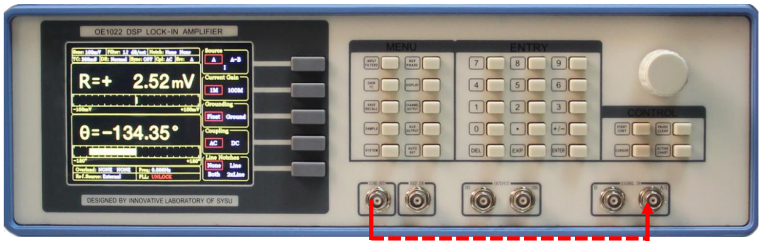
\includegraphics[scale=0.5]{D1-12}
			\caption{测量信号线连接图}\label{D1-12}
		\end{figure}
		
		\item 观察主界面中监测栏的 Overload 是否提示溢出:
		\begin{figure}[H]
			\centering
			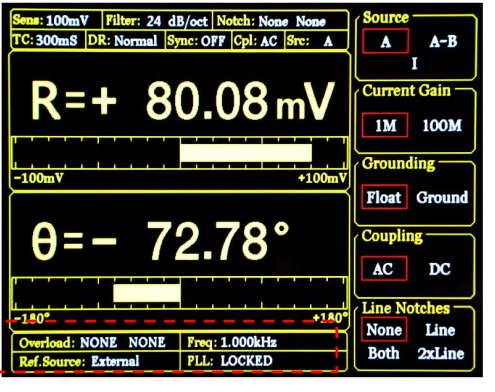
\includegraphics[scale=0.5]{D1-13}
			\caption{锁相放大器显示屏主界面监测栏}\label{D1-13}
		\end{figure}
	
		\item 若前级输入溢出,则显示 Overload: INPUT NONE;若放大溢出,则显示 Overload: NONE GAIN;若同时溢出,则显示 Overload: INPUT GAIN。
		
		\item 前级溢出时应立即减小数字信号发生器输出幅值,放大溢出应立即调节灵敏度(sensitivity)8值(OE1022输入端峰值高于1.7V或谷值低于-1.7V时发生前级溢出,且默认灵敏度值为100mV,因此本例中数字信号发生器输出幅值为 80mV 的正弦波时不会发生溢出,但是测量其他信号时要注意溢出情况)。调节灵敏度值的方法见下:
		
		\item 调节灵敏度值。按下前面板 GAIN/TC 按键进入子菜单。
		\begin{figure}[H]
			\centering
			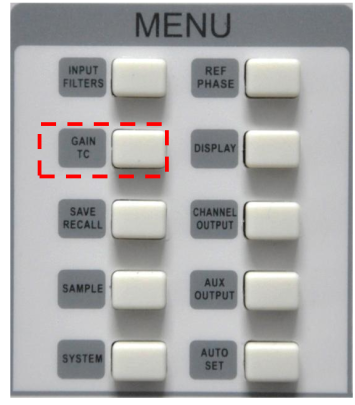
\includegraphics[scale=0.5]{D1-14}
			\caption{GAIN/TC 菜单位置}\label{D1-14}
		\end{figure}
	
		\item GAIN/TC 子菜单界面如图~\ref{D1-15}。
		\begin{figure}[H]
			\centering
			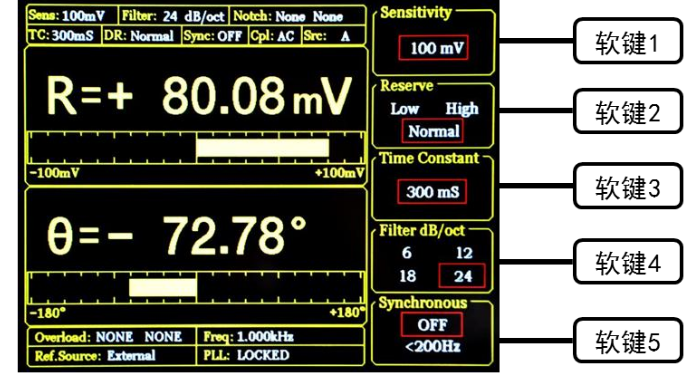
\includegraphics[scale=0.5]{D1-15}
			\caption{GAIN/TC 菜单参数显示}\label{D1-15}
		\end{figure}
		
		\item 按下软键 1 以选中 Sensitivity 功能,选中区域会有高亮显示,通过旋转旋钮调节 Sensitivity值,使测量信号值尽量满偏但不超量程。此处我们调节为 100mV 即可。至此,我们即简单测出了从函数信号发生器输出的正弦波幅值大小以及相位(测量结果参考值:R=80.08mV,$\theta=-72.78^\circ$,如果相位差显示其他值,可以点击ref 设signal 按软键1进行调节ref phase),比较示波器的读数和锁相放大器的 R 值,以理解 R 值的确切含义
		
		\item 主界面数据栏显示 R、$\theta$、X 及 Y 值。按下前面板 DISPLAY 按键进入子菜单
		\item DISPLAY 子菜单界面如下
		\begin{figure}[H]
			\centering
			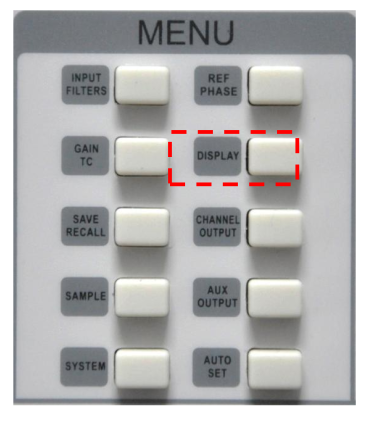
\includegraphics[scale=0.5]{D1-16}
			\caption{DISPLAY 菜单界面}\label{D1-16}
		\end{figure}
	
		\item 系统默认设置中,数据栏上方显示 R,下方显示 θ 值,通过以下介绍的方法可更改显示的数值:例如将上方显示的 R 值更改为采用 XY 坐标来显示 θ 值的方法:首先按软键 2,使其选中Top;再按软键 3 选中 Type,Type 区域此时高亮显示,通过调节旋钮可选择 Chart(XY 坐 标)或 Bar(数字百分比),我们选择 Chart;再按软键 3 选 Trace,Trace 区域此时高亮显示,通过调节旋钮可选择显示 R、$\theta$、X、Y,我们选择 $\theta$。然后按下前面板右下角处的 START CONT 按键,此时图像开始生成
		
		\item 通过改变$\theta$值,观察 X、Y 是如何相应地改变
		\begin{table}[H]
			\centering
			\caption{$\theta$与X,Y关系}
			\begin{tabular}{| c | p{2cm} | p{2cm} | p{2cm} |}
				\hline
				次数 & $\theta$ & X(mV) & Y(mV) \\
				\hline
				1 &  &  &  \\
				\hline
				2 &  &  &  \\
				\hline
				3 &  &  &  \\
				\hline
				4 &  &  &  \\
				\hline
				5 &  &  &  \\
				\hline
				6 &  &  &  \\
				\hline
			\end{tabular}
		\end{table}
		
		\item 可以更改检测栏的内容使其实时显示 R、$\theta$、X、Y 值。方法:按下前面板 DISPLAY 按键进入子菜单,再按软键 1 将 Monitor 设置中从 Setting 切换为 Output,此时监测栏显示 R、$\theta$、 X 和 Y 的值
		
		\item 影响相位差测量的因素
		改变不同的频率值,看看 R、X、Y、和$\theta$分别有什么变化?为什么?[提示,可用 sweep 设置参考信号。
		\begin{table}[H]
			\centering
			\caption{$\theta$与X,Y关系}
			\begin{tabular}{|  p{2cm} | p{2cm} | p{2cm} | p{2cm} | p{2cm} |}
				\hline
				频率 & $\theta$ & X(mV) & Y(mV) & R \\
				\hline
				 &  &  &  & \\
				\hline
				 &  &  &  & \\
				\hline
				 &  &  &  & \\
				\hline
				 &  &  &  & \\
				\hline

			\end{tabular}
		\end{table}
		
		
		\item ) 在 1 kHz 至 100kHz 范围内观察一米电缆对相位差的影响。
		设置某一参考信号频率,记录其相位差$\theta_0(f)$值,然后延长
		sine out 到 signal in 的电缆,记录延长电缆后的相位差$\theta_e(f)$)值,并计算$\delta\theta(f)=\theta_e(f)-\theta_0(f)$
		\begin{table}[H]
			\centering
			\caption{$\theta$与X,Y关系}
			\begin{tabular}{|  p{2cm} | p{2cm} | p{2cm} | p{2cm} |}
				\hline
				频率 & $\theta_0(f)$ & $\theta_e(f)$ & $\delta\theta(f))$ \\
				\hline
				&  &  &   \\
				\hline
				&  &  &   \\
				\hline
				&  &  &   \\
				\hline
				&  &  &   \\
				\hline
				
			\end{tabular}
		\end{table}
		操作验证:是否可以先测量不同频率下的一组$\theta_0(f)$值,然后再延长电缆,再测量对应频率下的一组$\theta_e(f)$)值?能定性解释$\theta_0(f)$吗?
\end{enumerate}
		\subsubsection{不同时间常数、陡降、动态储备下观测滤波器效果}
		\begin{enumerate}[(1)]
		\item 断开所有与机箱连接的信号线,接入电源,打开电源开关,此时系统处于默认设置状态。
		在前面板上选择 REF/PHASE 子菜单,Ref.source 设置为“Internal”;Ref.frequency 为默认
		值“1.000kHz”;选择进入“Sine Output”下级菜单,扫描类型 Sweep Type 设置为“Fixed”,通
		过数字键盘在 Voltage 中输入“0.05”,得到幅值为 50m$V_{rms}$、频率为 1.000kHz 的正弦信号。
		\item 用 BNC-BNC 信号线连接 OE1022 前面板 SINE OUT 输出接口和 SIGNAL IN 的 A/I 接口,
		OE1022 前面板 CH1 接口和示波器输入接口。
		\item 调节灵敏度值,本例中数字信号发生器输出有效值为 50mVrms 的正弦波,相位(phase)
		设置为 60deg,灵敏度设置为 100mV 即可。
		\item 按下 OE1022 前面板的 GAIN/TC 按键,调节时间常数和陡降,设置时间常数为 30μs,陡
		降为 6dB/oct。
		\item 按下 OE1022 前面板 CHANNEL OUTPUT 按键,进入子菜单,在 Output 选项中选择 CH1, 在 Speed 选项中选择 Fast,Source 选项默认为 R(Fast 模式下输出源可选择 R、X、Y,
		Slow 模式下输出源可选择 R、X、Y、Rh1、Xh1、Yh1、Rh2、Xh2、Yh2、Noise、$\theta$、$\theta$h1、 $\theta$h2),Offset\&Expand 中默认 Offset 为 0,Expand 为 1。
		\item 在示波器上调节时基、输入通道设置等,可观测到在 30μs 时间常数和 6dB/oct 陡降下channel out 输出 R 值波形.(示波器所测量的 CH1 输出信号频率与设定信号频率是什么关系?时间常数大小对此
		有何影响?为什么?)
		
		\item 在 OE1022 的 Channel out 菜单中设置 Source 为 X、Y,在示波器上观测
		
		\item 在 OE1022 的 Gain/TC 菜单中,对时间常数进行改变,时间常数可选择 10$\mu$s、30$\mu$s、100$\mu$s、
		300$\mu$s……10s、30s,通过增大时间常数的值能够使系统的输出端更稳定,也能减轻输入端
		噪声对输出端的影响。时间常数除了对系统的稳定性和精度有影响外,还会影响系统的响
		应时间,时间常数还决定噪声测量时的等效噪声带宽(ENBW)。在此特别说明一下,等效
		噪声带宽指的并不是滤波器的-3 dB 带宽,它指的是对高斯噪声10的有效带宽。观察示波
		器波形,并给出:时间常数为多少个信号周期时,才能观察到稳定的直流输出?
		
		\item 在 OE1022 的 Gain/TC 菜单中,对滤波器陡降进行改变。在同样的测量准确度下,请分别
		选择 6dB/oct、12dB/oct、18dB/oct、24dB/oct 四档,在 TC 不大于 30$\mu$s 的情况下,观察示
		波器波形的变化。
\end{enumerate}
		\subsubsection{制定方案,观测不同时间常数下,输出信号对输入信号变化的响应。}
		\begin{enumerate}
			\item 分别设置时间常数:30$\mu$s、100$\mu$s、
			300$\mu$s、10ms、100ms、300ms
			\item 改变 SINE OUT 幅值设定,每个时间常数改变幅值为$V_{rms}$从 $50mV_{rms}$和$70mV_{rms}$
			\item 用“START CONT”激活 chart 图以观察改变前后的曲线来确定其输出响应,并记录图形
		
		\item 在 OE1022 的 Gain/TC 菜单中,对滤波器陡降进行改变。在同样的测量准确度下,分别选择 6dB/oct、12dB/oct、18dB/oct、24dB/oct 四档,观察在输入信号改变时,输出信号对输入信号变化的响应;并理解滤波器陡降的作用
	        \end{enumerate}
                	\subsubsection{不同的噪声水平下,考察 OE1022 如何选用合适的动态储备测量信号?}
	在 OE1022 的 Gain/TC 菜单中,对动态储备进行设置,可设置为 Low、High、Normal
	三档之一。动态储备表示锁相放大器对噪声容忍程度的大小,OE1022 动态储备可大于
	100 dB,高的动态储备会产生输出噪声和漂移,当动态储备较高时,由于模数转换器的噪声存在导致输出误差增加。由于所有的信号源都存在本底噪声,固在 PSD 提取信号过程
	中就会掺杂着噪声,如果噪声很大,在高动态储备测量中就会产生较大的输出误差。如果
	外部噪声较小,则其输出主要是受 OE1022 自身噪声影响。这时可以通过降低动态储备和
	直流增益可以减小输出误差。因此,在实际应用中应尽量使用低动态储备。默认配置下系
	统会根据输入信号的 R 值自动调整所需要的最小动态范围。观察示波器波形变化,给出结
	论。
        \subsubsection{外部输入参考信号}
        (配备信号发生器或另一台锁相放大器的正弦输出)
。用信号发生器产生正弦信号作为外
部参考信号,并用三通将信号用 BNC 线分别接入 REF IN,和 signal in 的 A/I,在锁相放大器
参数设置 Ref.source->external;重复部分操作(自己定测什么、测量参数的范围、测量点数、
是否截图等)
。
【注意:外部参数信号要求峰值 100mV 以上。
】
对于 OE1022 锁相放大器的信号处理质量,用内部参考信号好还是外部参考信号好?
	\subsection{强噪声背景下的弱信号检测——应用体验}
	\subsubsection{用示波器观察教学实验箱噪声发生器输出的噪声是否白噪声?记录时域和频域的图谱来说明。}

	\subsubsection{比较 OE1022 与示波器对不同信号强度和信噪比的测量结果}
	\begin{enumerate}
		\item 使用 OE1022 产生频率 1kHz,幅值为 100m$V_{rms}$(0.282Vpp)的正弦波信号;
		\item 对锁相放大器 OE1022 进行以下设置:
		
		进入 INPUT FLTERS 菜单,设置 Source 为 A;
		
		进入 GAIN TC 菜单,设置 Sensitivity 为 500mV,Reserve 为 Normal,Time Constant
		为 1s,Filter dB/oct 为 24dB;
		
		进入 REF PHASE 菜单,设置 Ref. source 为 Internal;
		\item 使用 BNC-BNC 信号线连接 OE1022 的“SINE OUT”接口与实验箱本实验框图中的
		“VIN”接口;
		\item 通过分线器,使用 BNC-BNC 信号线将实验箱本实验框图中的“VOUT”接口分别连接
		到 OE1022 的“A/I”接口、和示波器输入端;
		\item 读取 OE1022 测到的 R 值,即为被噪声信号淹没的正弦信号有效值;
		\item 改变 OE1022 产生正弦波有效值,在不同信噪比下重复上述测量;
		
		\begin{table}[H]
			\centering
			\begin{tabular}{ | p{2cm} | p{2cm} | p{2cm} | p{2cm} | p{2cm} |}
				\hline
				 正弦波$V_in$幅值(m$V_{rms}$) & 噪声信号大小(m$V_{rms}$) & 信噪比(dB)&锁相放大器测量R(m$V_{rms}$) & 示波器测量值(m$V_{rms}$)\\
				\hline
				  &  & & &  \\
				\hline
				  &  &  & & \\
				\hline
				  &  &  & & \\
				\hline
				  &  &  & & \\
				\hline
			\end{tabular}
		\end{table}
	\end{enumerate}
        \subsection{实验过程中遇到的问题记录}
        由于示波器的阻抗设置不对,图形出现了截断。

        \subsection{实验原始记录与签名}
        \cpicn{0.2}{1}{数据的原始记录}
        \cpicn{0.2}{2}{数据的原始记录}
        \cpicn{0.2}{3}{数据的原始记录}
        \cpicn{0.2}{4}{数据的原始记录}
        \cpicn{0.2}{5}{数据的原始记录}
        \cpicn{0.2}{6}{数据的原始记录}
\newpage
\section{分析与讨论}
\begin{tabular}{|p{7em}|p{7em}|p{7em}|p{7em}|}
	\hline 
	专业:     &Physics       &年级:      & 17     \\
	\hline
	姓名:& 徐昊霆 &学号:&17353071  \\
	\hline
	日期&  \today              & &  \\
	\hline	
	评分 & & 教师签名 & \\
	\hline
\end{tabular}
\subsection{实验数据分析}
\subsubsection{测量信号R、$\theta$、X 以及 Y 值,并验证它们之间的关系}
在实验中,我们使用BNC-BNC信号线连接了SINE OUT输出接口和SIGNAL IN 的A/I接口,通过改变参考信号相位,我们获得的$R,\theta,X,Y$数据见上节附录。通过数据软件使用最小二乘法~~\cite{error}使用正弦曲线对数据$\theta,X$进行拟合,如~\cref{theta&x_1}所示。
\cpicn{0.5}{theta&x_1}{$\theta$和$X$的拟合曲线}
在拟合过程中,我们使用拟合系数$R^2$来表征拟合的好坏,设待拟合数据为$y$,拟合出来的对应曲线上的点为$f$,则拟合系数定义为
\beq
R^2 = 1-\frac{\sum_i(y_i - f_i)^2}{\sum_i (y_i-\bar{y})^2}
\eeq
由上述公式我们计算得到,拟合曲线的拟合系数为
\beq
R^2 = 0.99999
\eeq
通过数据软件使用最小二乘法使用正弦曲线对数据$\theta,Y$进行拟合,如~\cref{theta&y_1}所示。
\cpicn{0.5}{theta&y_1}{$\theta$和$Y$的拟合曲线}
在拟合过程中,我们使用拟合系数$R^2$来表征拟合的好坏,设待拟合数据为$y$,拟合出来的对应曲线上的点为$f$,则拟合系数定义为
\beq
R^2 = 1-\frac{\sum_i(y_i - f_i)^2}{\sum_i (y_i-\bar{y})^2}
\eeq
由上述公式我们计算得到,拟合曲线的拟合系数为
\beq
R^2 = 0.99999
\eeq
可见,$X,Y$确实随着$\theta$的变化满足正弦和余弦的关系。
\subsubsection{频率的变化对于相位差,$X,Y,R$的影响}
在本实验中我们通过改变频率,固定其他因素不变,探究频率的增加对于相位差和$X,Y,R$的影响。数据见实验数据与记录的附录部分,我们首先研究频率变化对于相位差的影响。实验中测得频率与相位差的关系如~\cref{freq&theta}所示。
\cpicn{0.5}{freq&theta}{改变频率时,相位差随着频率的变化}
由实验数据可以看到,随着频率的升高,相位差与频率有着线性关系,经过最小二乘法进行线性拟合,得到的频率与相位差的表达式为
\beq
\theta = kf+b
\eeq
其中,
\bea
k &=& 0.01\pm 0.01 \\
b &=& 0.01\pm 0
\eea
为什么频率的变化会引起相位差的变化?我们要清楚,这里的相位差指的是调制后的信号与解调信号的相位差,而解调信号一般是由输入的信号通过某种物理机制产生的。因此,由于电缆的存在,信号在电缆中传播会引起额外的相位差,这一部分的相位差贡献到了调制后的信号的相位中,因此产生了相位差。根据介质中的麦克斯韦方程组(例如,参见~\cite{electromagnetic})
\bea
\nabla \cdot \vec{E} &=& \rho/\epsilon \\
\nabla \times \vec{E} &=& -\frac{\partial \vec{B}}{\partial t} \\
\nabla \cdot \vec{B} &=& 0\\
\nabla \times \vec{B} &=& \mu\vec{j} + \mu\epsilon \frac{\partial E}{\partial t}
\eea
利用公式
\beq
\nabla\times( \nabla\times \vec{E} ) =  \nabla(\nabla \cdot \vec{E}) - \nabla^2 \vec{E}
\eeq
将麦克斯韦方程组带入上式两边,利用欧姆定律,并取$\rho = 0 $,得到
\beq
\frac{\partial^2 \vec{E} }{\partial t^2}+\mu \sigma \partial_t \vec{E} - \frac{1}{\mu\epsilon} \nabla^2 \vec{E} =0
\eeq
上式实际上是一个波动方程,$\mu \sigma \partial_t \vec{E}$可以看做阻尼项,如果$\sigma$很小,则阻尼很小,实际上阻尼意味着一个弛豫时间,如果知道输入信号的强度和锁相放大器接受的信号强度,可以测量这个弛豫时间,进而测量金属电导率。所以我们得到,电磁场在电缆中传播的速度为
\beq
v = \frac{1}{\mu \epsilon} \simeq 10^8 \,\mathrm{m/s}
\eeq
因为电缆有$1$m长,所以在电缆的传播过程导致了时间差
\beq
\Delta t = \frac{l}{v}
\eeq
进而造成了相位改变
\beq
\omega \Delta t = 2\pi \nu \Delta t
\eeq
进而造成了相位差的改变。所以当相位改变大于相位分辨率时,就能测出由上述效应导致的相位差变化。


接下来研究频率变化对于$X$的影响。实验中测得频率与$X$的关系如~\cref{freq&X}所示。
\cpicn{0.5}{freq&X}{改变频率时,$X$的值随着频率的变化}
由实验数据可以看到,随着频率的升高,相位差与频率有着线性关系,经过最小二乘法进行线性拟合,得到的频率与$X$的表达式为
\beq
X=kf+b
\eeq
其中,
\bea
k &=& 0.01\pm 0.01 \\
b &=& 0.01\pm 0
\eea

接下来研究频率变化对于$Y$的影响。实验中测得频率与$Y$的关系如~\cref{freq&Y}所示。
\cpicn{0.5}{freq&Y}{改变频率时,$Y$的值随着频率的变化}
由实验数据可以看到,随着频率的升高,相位差与频率有着线性关系,经过最小二乘法进行线性拟合,得到的频率与$Y$的表达式为
\beq
Y=kf+b
\eeq
其中,
\bea
k &=& 0.01\pm 0.01 \\
b &=& 0.01\pm 0
\eea

接下来研究频率变化对于$R$的影响。实验中测得频率与$Y$的关系如~\cref{freq&R}所示。
\cpicn{0.5}{freq&R}{改变频率时,$R$的值随着频率的变化}
由实验数据可以看到,随着频率的升高,相位差与频率有着线性关系,经过最小二乘法进行线性拟合,得到的频率与$R$的表达式为
\beq
R=kf+b
\eeq
其中,
\bea
k &=& 0.01\pm 0.01 \\
b &=& 0.01\pm 0
\eea

\subsubsection{探究一米长度的电缆对于相位差的影响}
在实验中,我们先设定频率,然后更换1m长和2m长的电缆,分别测定他们的相位差,之后将长电缆与短电缆的相位差值相减,得到他们的差。实验中测得相位差的差值随着频率的升高如~\cref{one_meter}所示。
\cpicn{0.5}{one_meter}{更换1m长和2m长电缆得到的相位差的差值随着频率的变化曲线。}
由曲线可以发现,随着频率的升高,两种BNC线测到的相位差的绝对值随着频率的升高而现行增加。根据前面的理论(式~\cref{phase})预测一致。

当然,这一相位差的变化并不是由于信号传播具有速度一个因素引起的,由于导线本身具有阻抗,这一效应也可以导致相位差的移动。由于导线的阻抗本身未知,所以这一效应计算比较困难。但是实验中,我们确实观测到,相位差的移动随着频率成正比。

操作验证:如果更改实验步骤的顺序,先固定电缆不变,不断改变频率,然后再更换电缆,改变频率,测得的相位差的变化就没有这么好的线性关系了。这是由于改变了频率,导致锁相放大器内部的触发机制重置,这一部分的效应也贡献在相位差中,实验中测到的就不是纯粹由于电缆延长而引起的相位差的变化了。

\subsubsection{不同时间常数、陡降、动态储备下观测滤波器效果}

\begin{enumerate}
  \item 首先我们将陡降设置为$6dB$,从而观察时间常数改变时,输出波形的改变。实验中,我们发现当时间常数大概为$300\mathrm{ms}$时,观察到了稳定的直流输出。参数设置和观察到的图形如下面的一系列图所示。
\cpicn{0.05}{shuju/1/settings}{当时间常数为$300\mathrm{ms}$时,对于输出信号参数的设置。}
\begin{figure}[H]
	\centering
	\subfloat{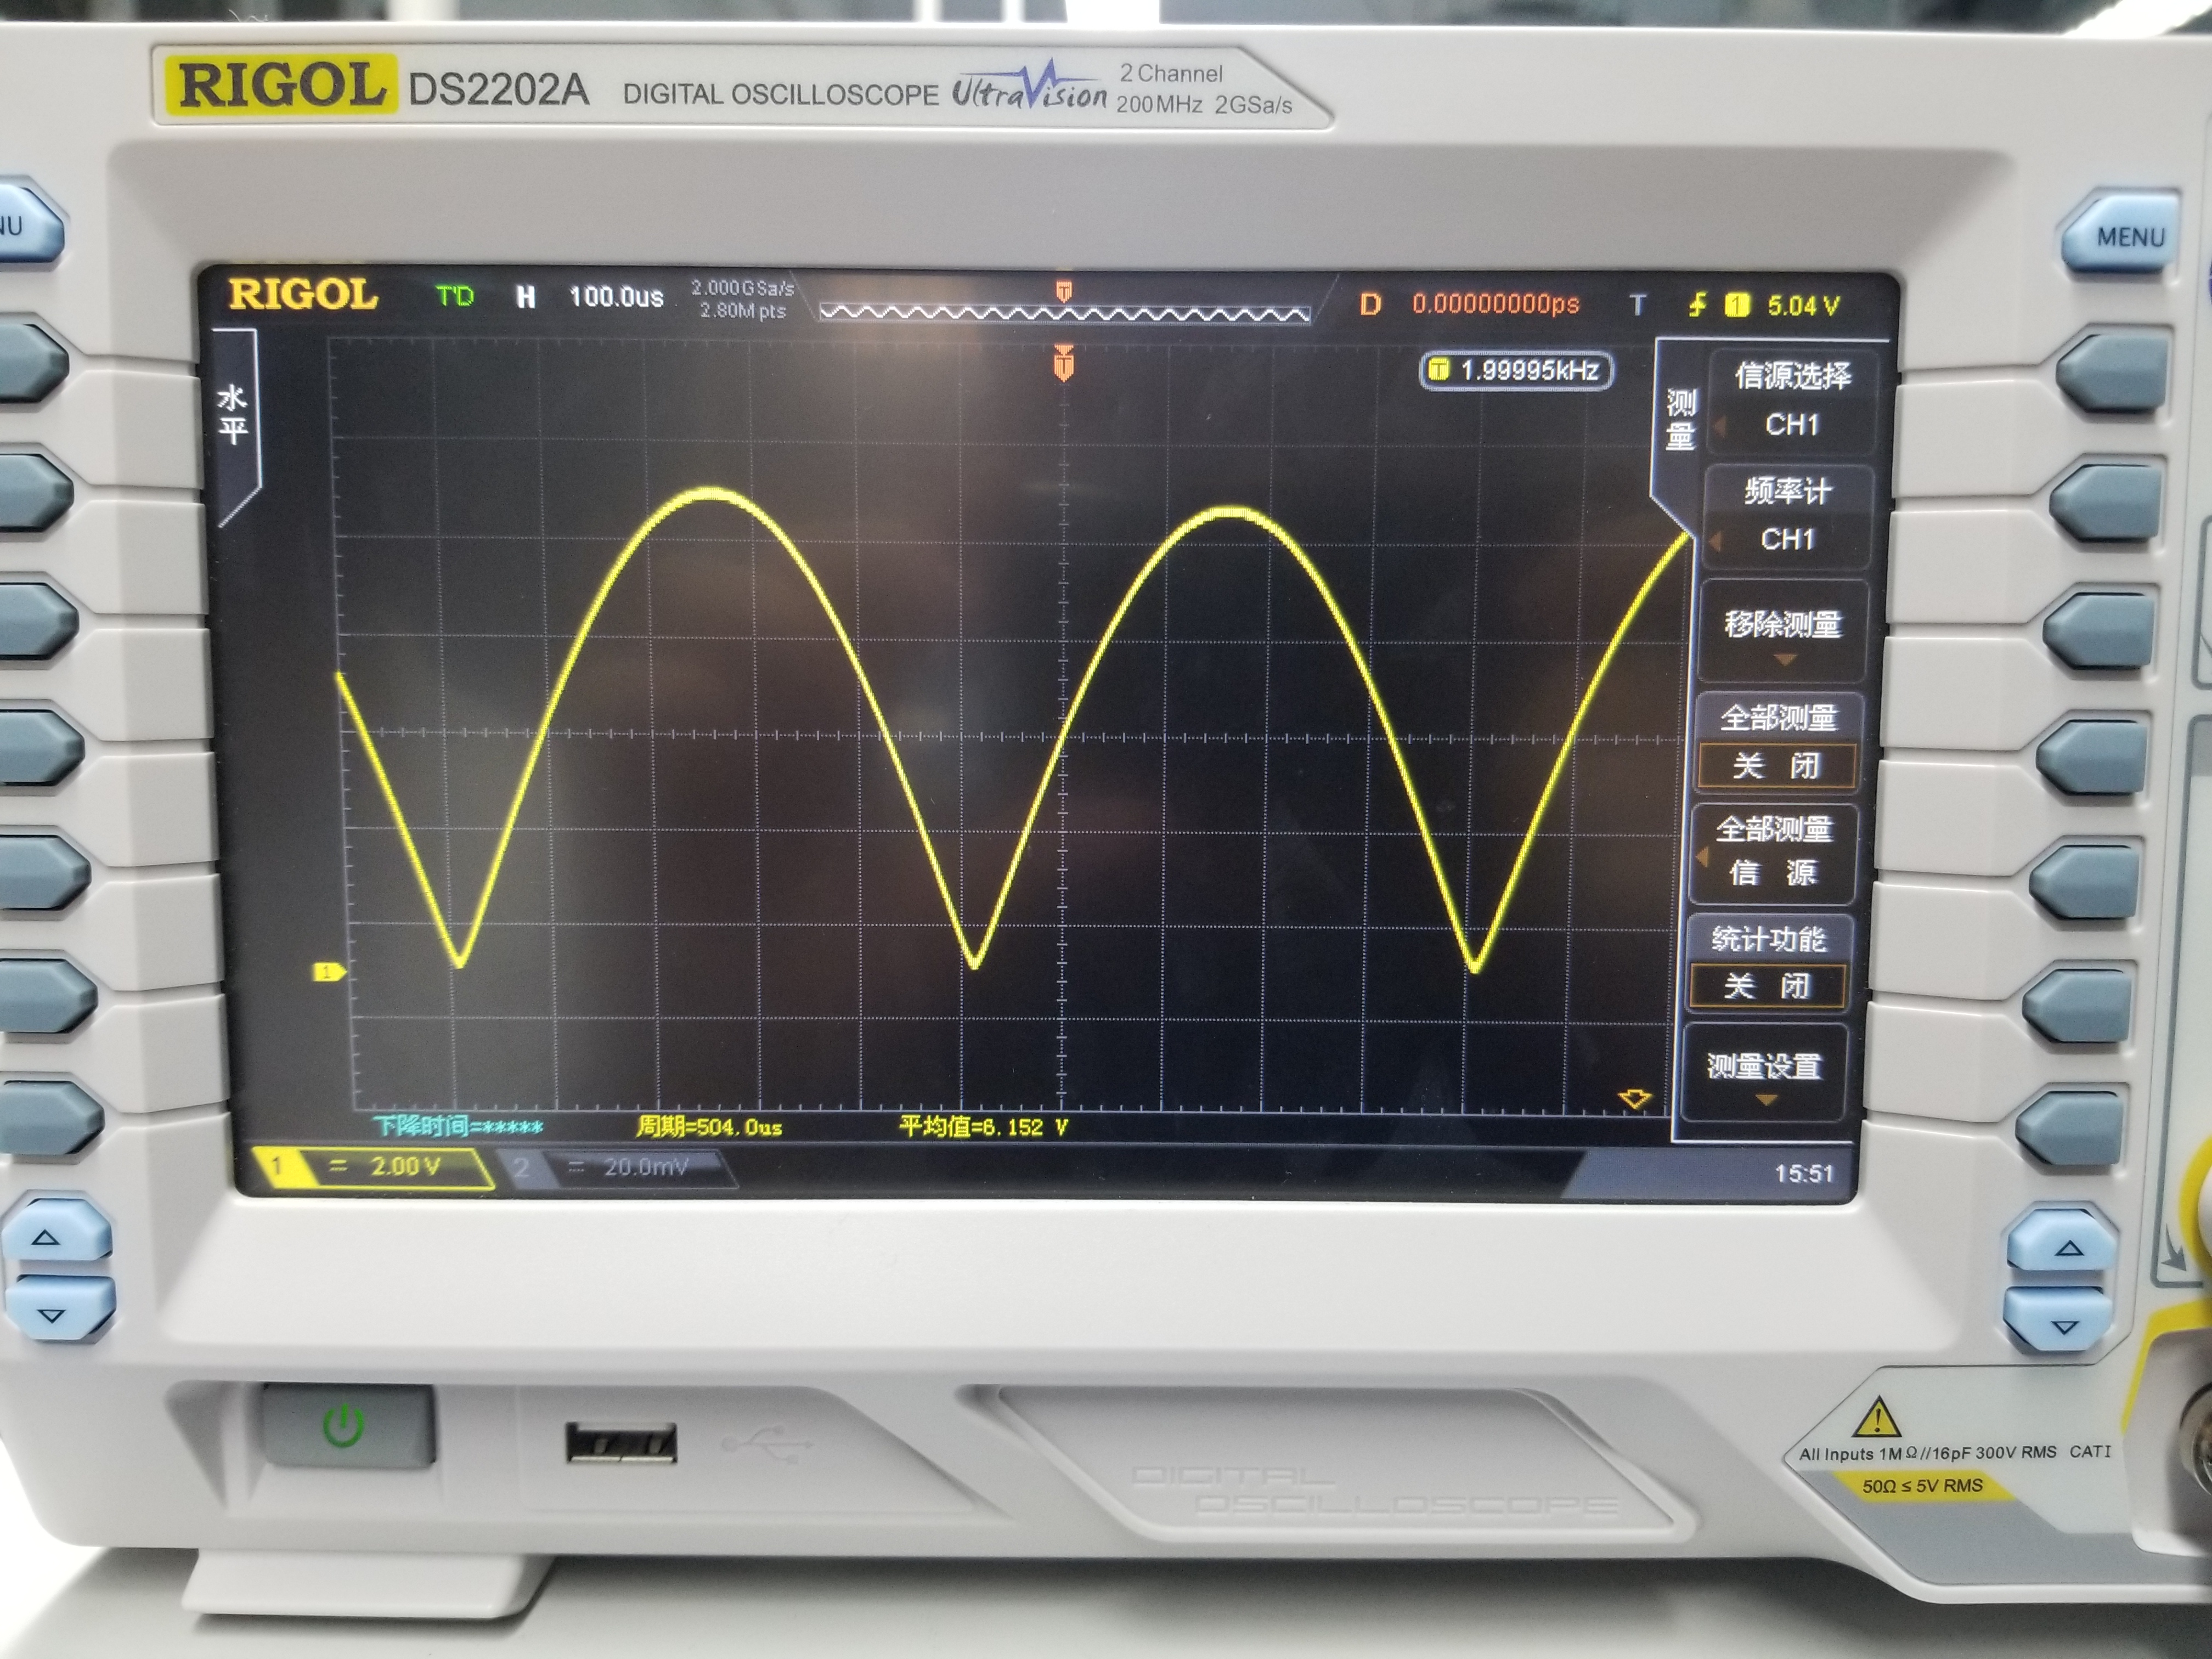
\includegraphics[width=1.5in]{shuju/1/6db_30us_R}}\quad
        \subfloat{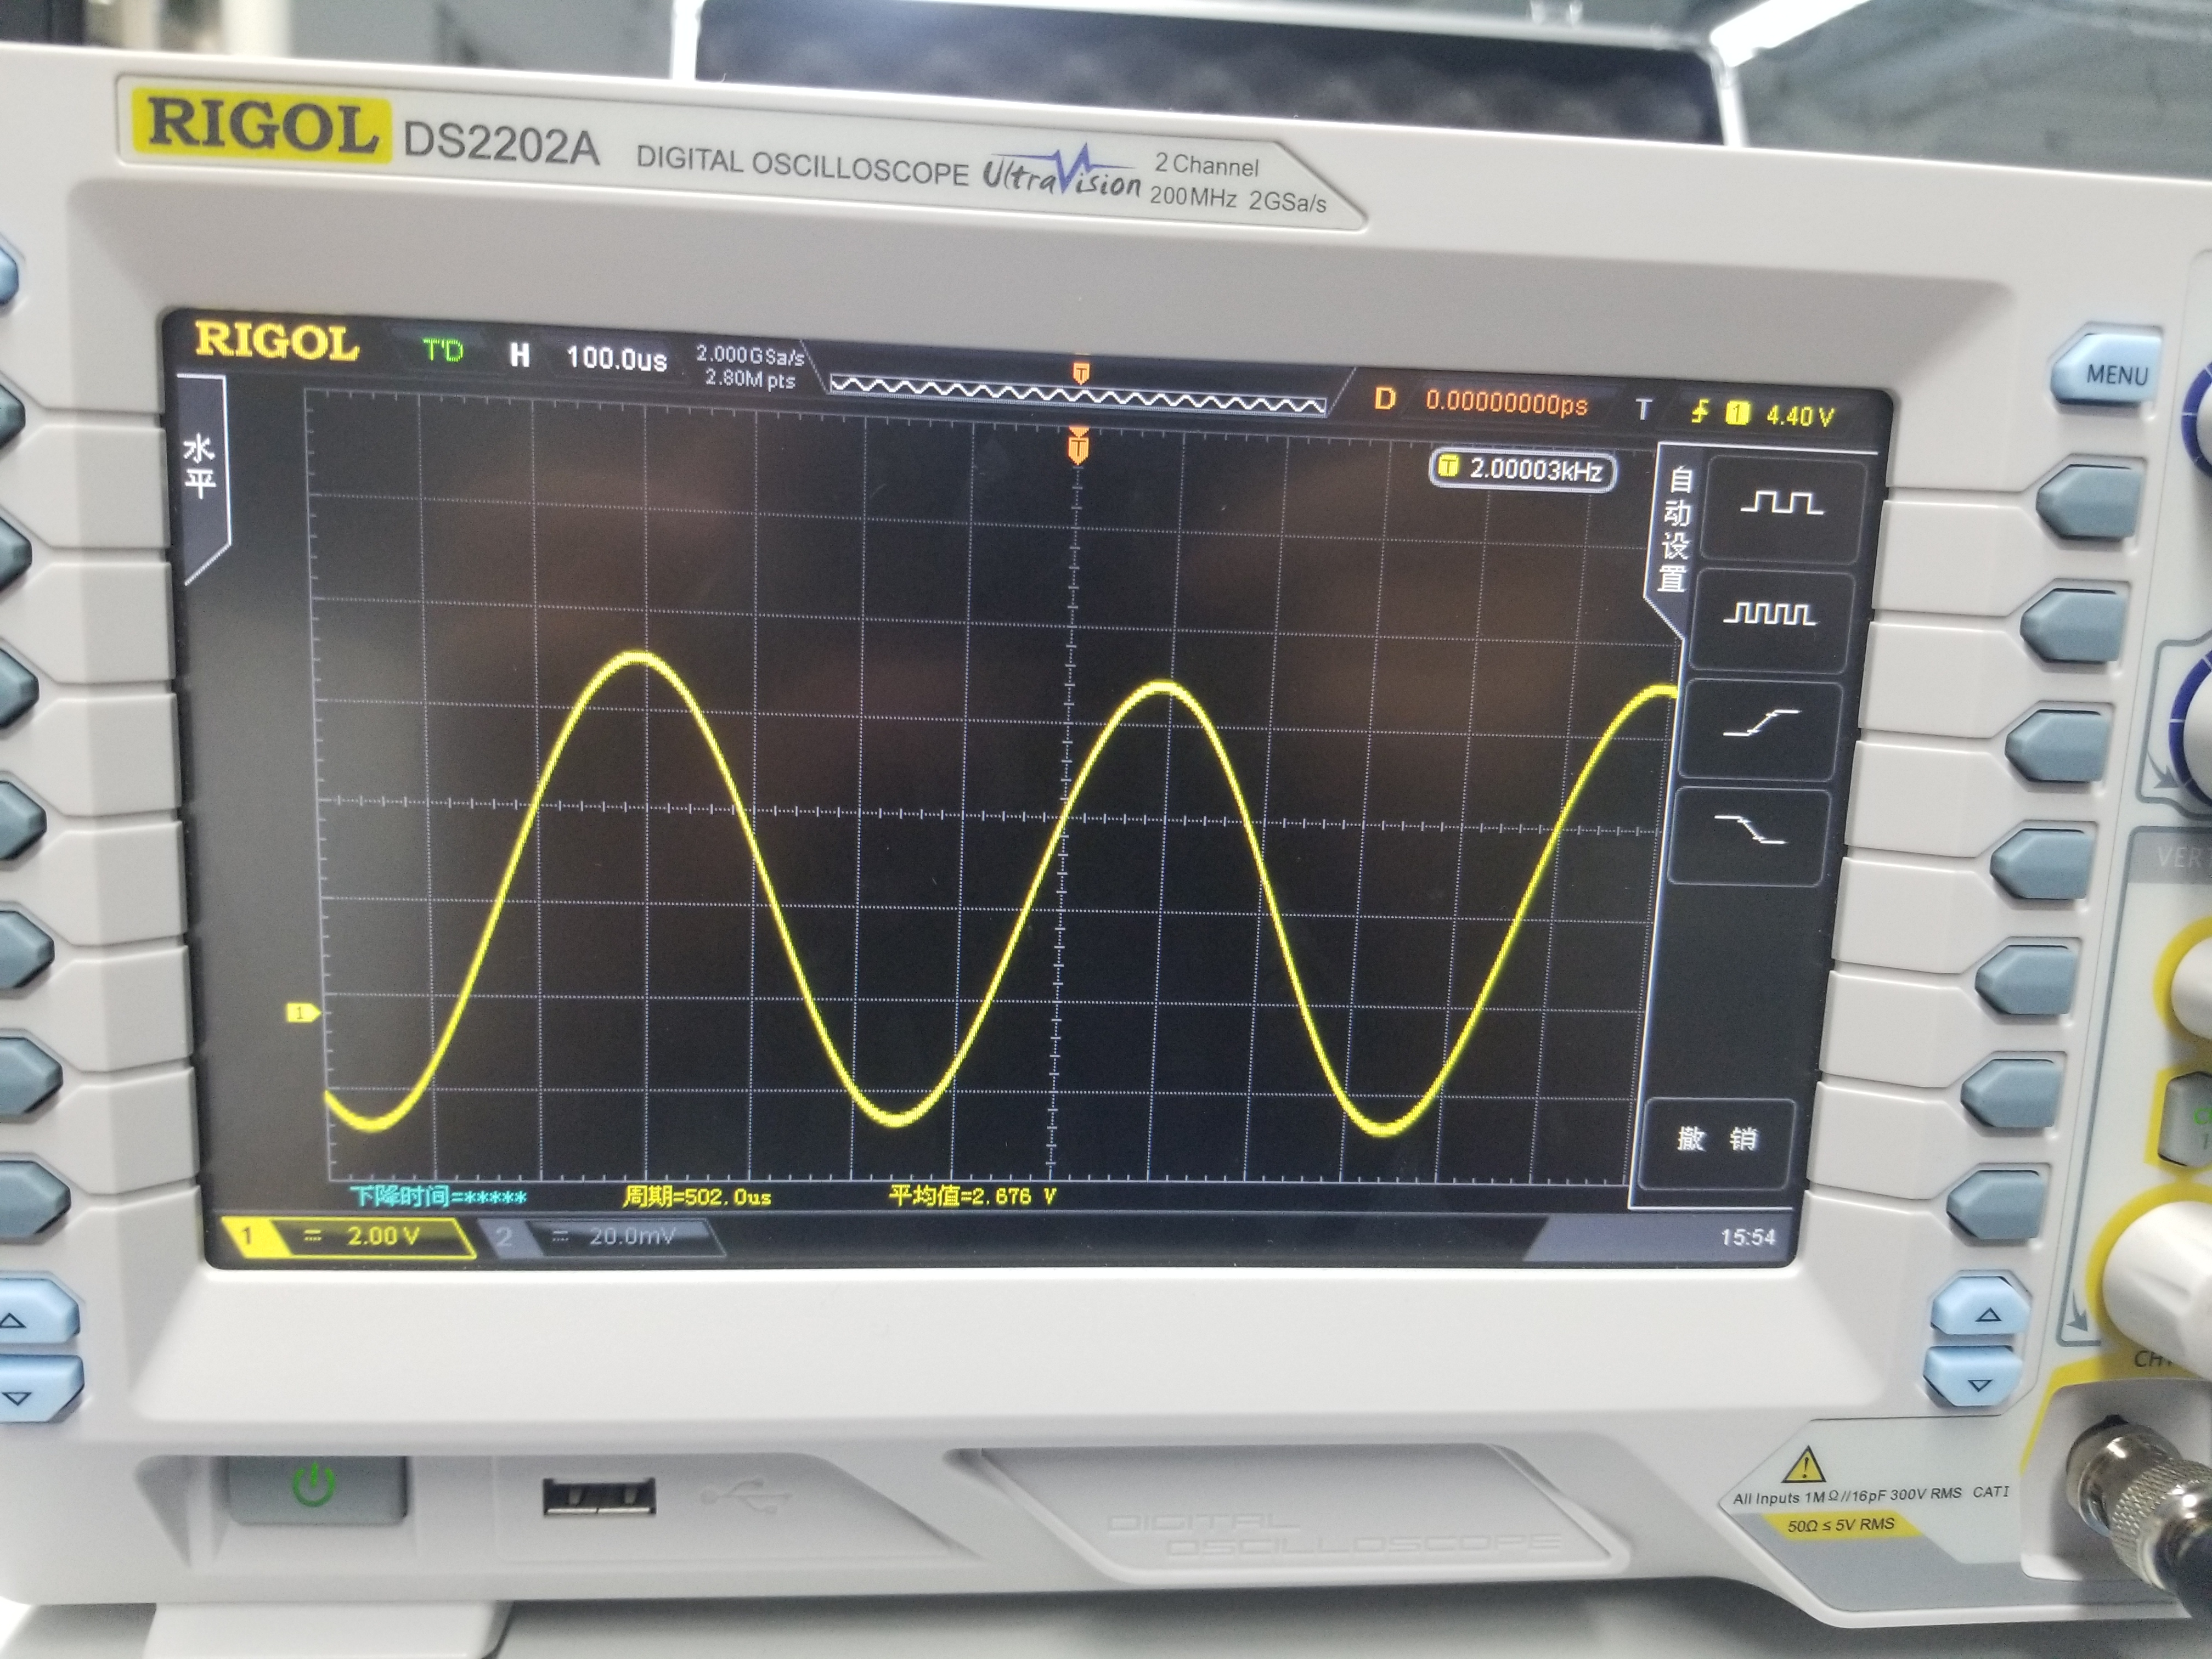
\includegraphics[width=1.5in]{shuju/1/6db_30us_x}}\quad
	\subfloat{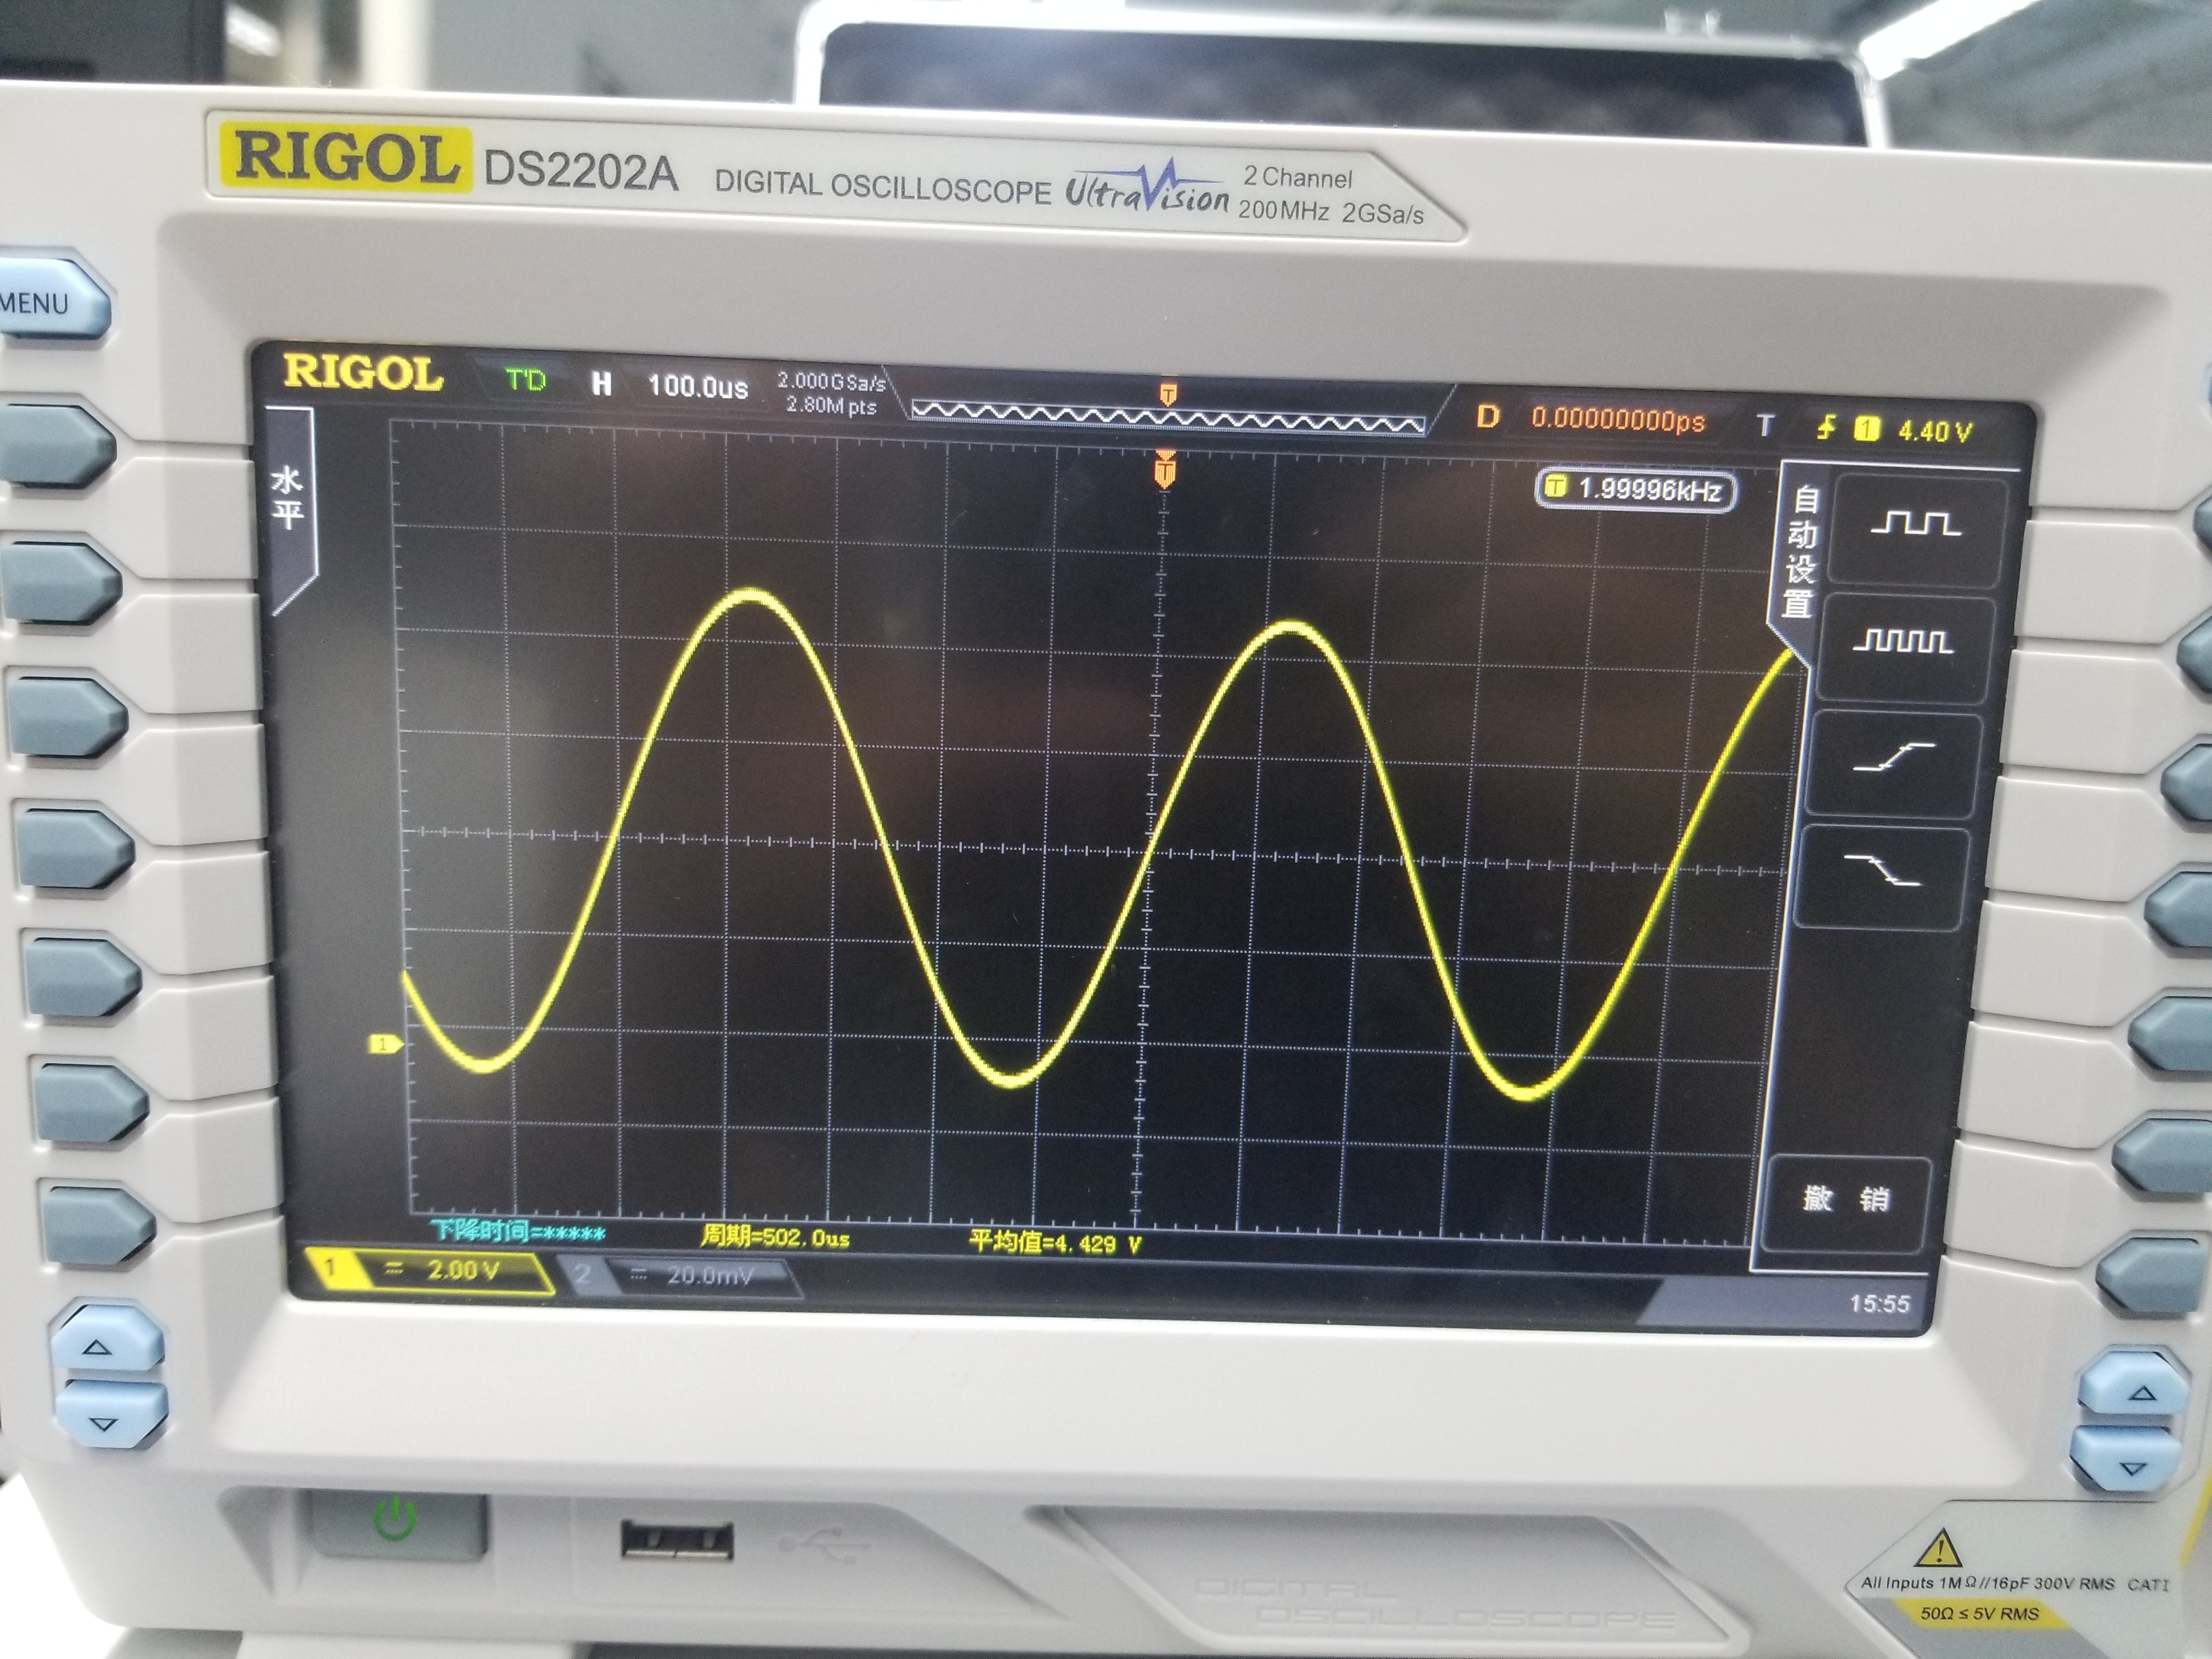
\includegraphics[width=1.5in]{shuju/1/6db_30us_y}}\\	
	\caption{陡降设置为$6dB$,时间常数设置为$30\mathrm{\mu s}$时示波器上的波形,从左边到右边依次为$X,Y,R$的波形。}
\end{figure}
\begin{figure}[H]
	\centering
	\subfloat{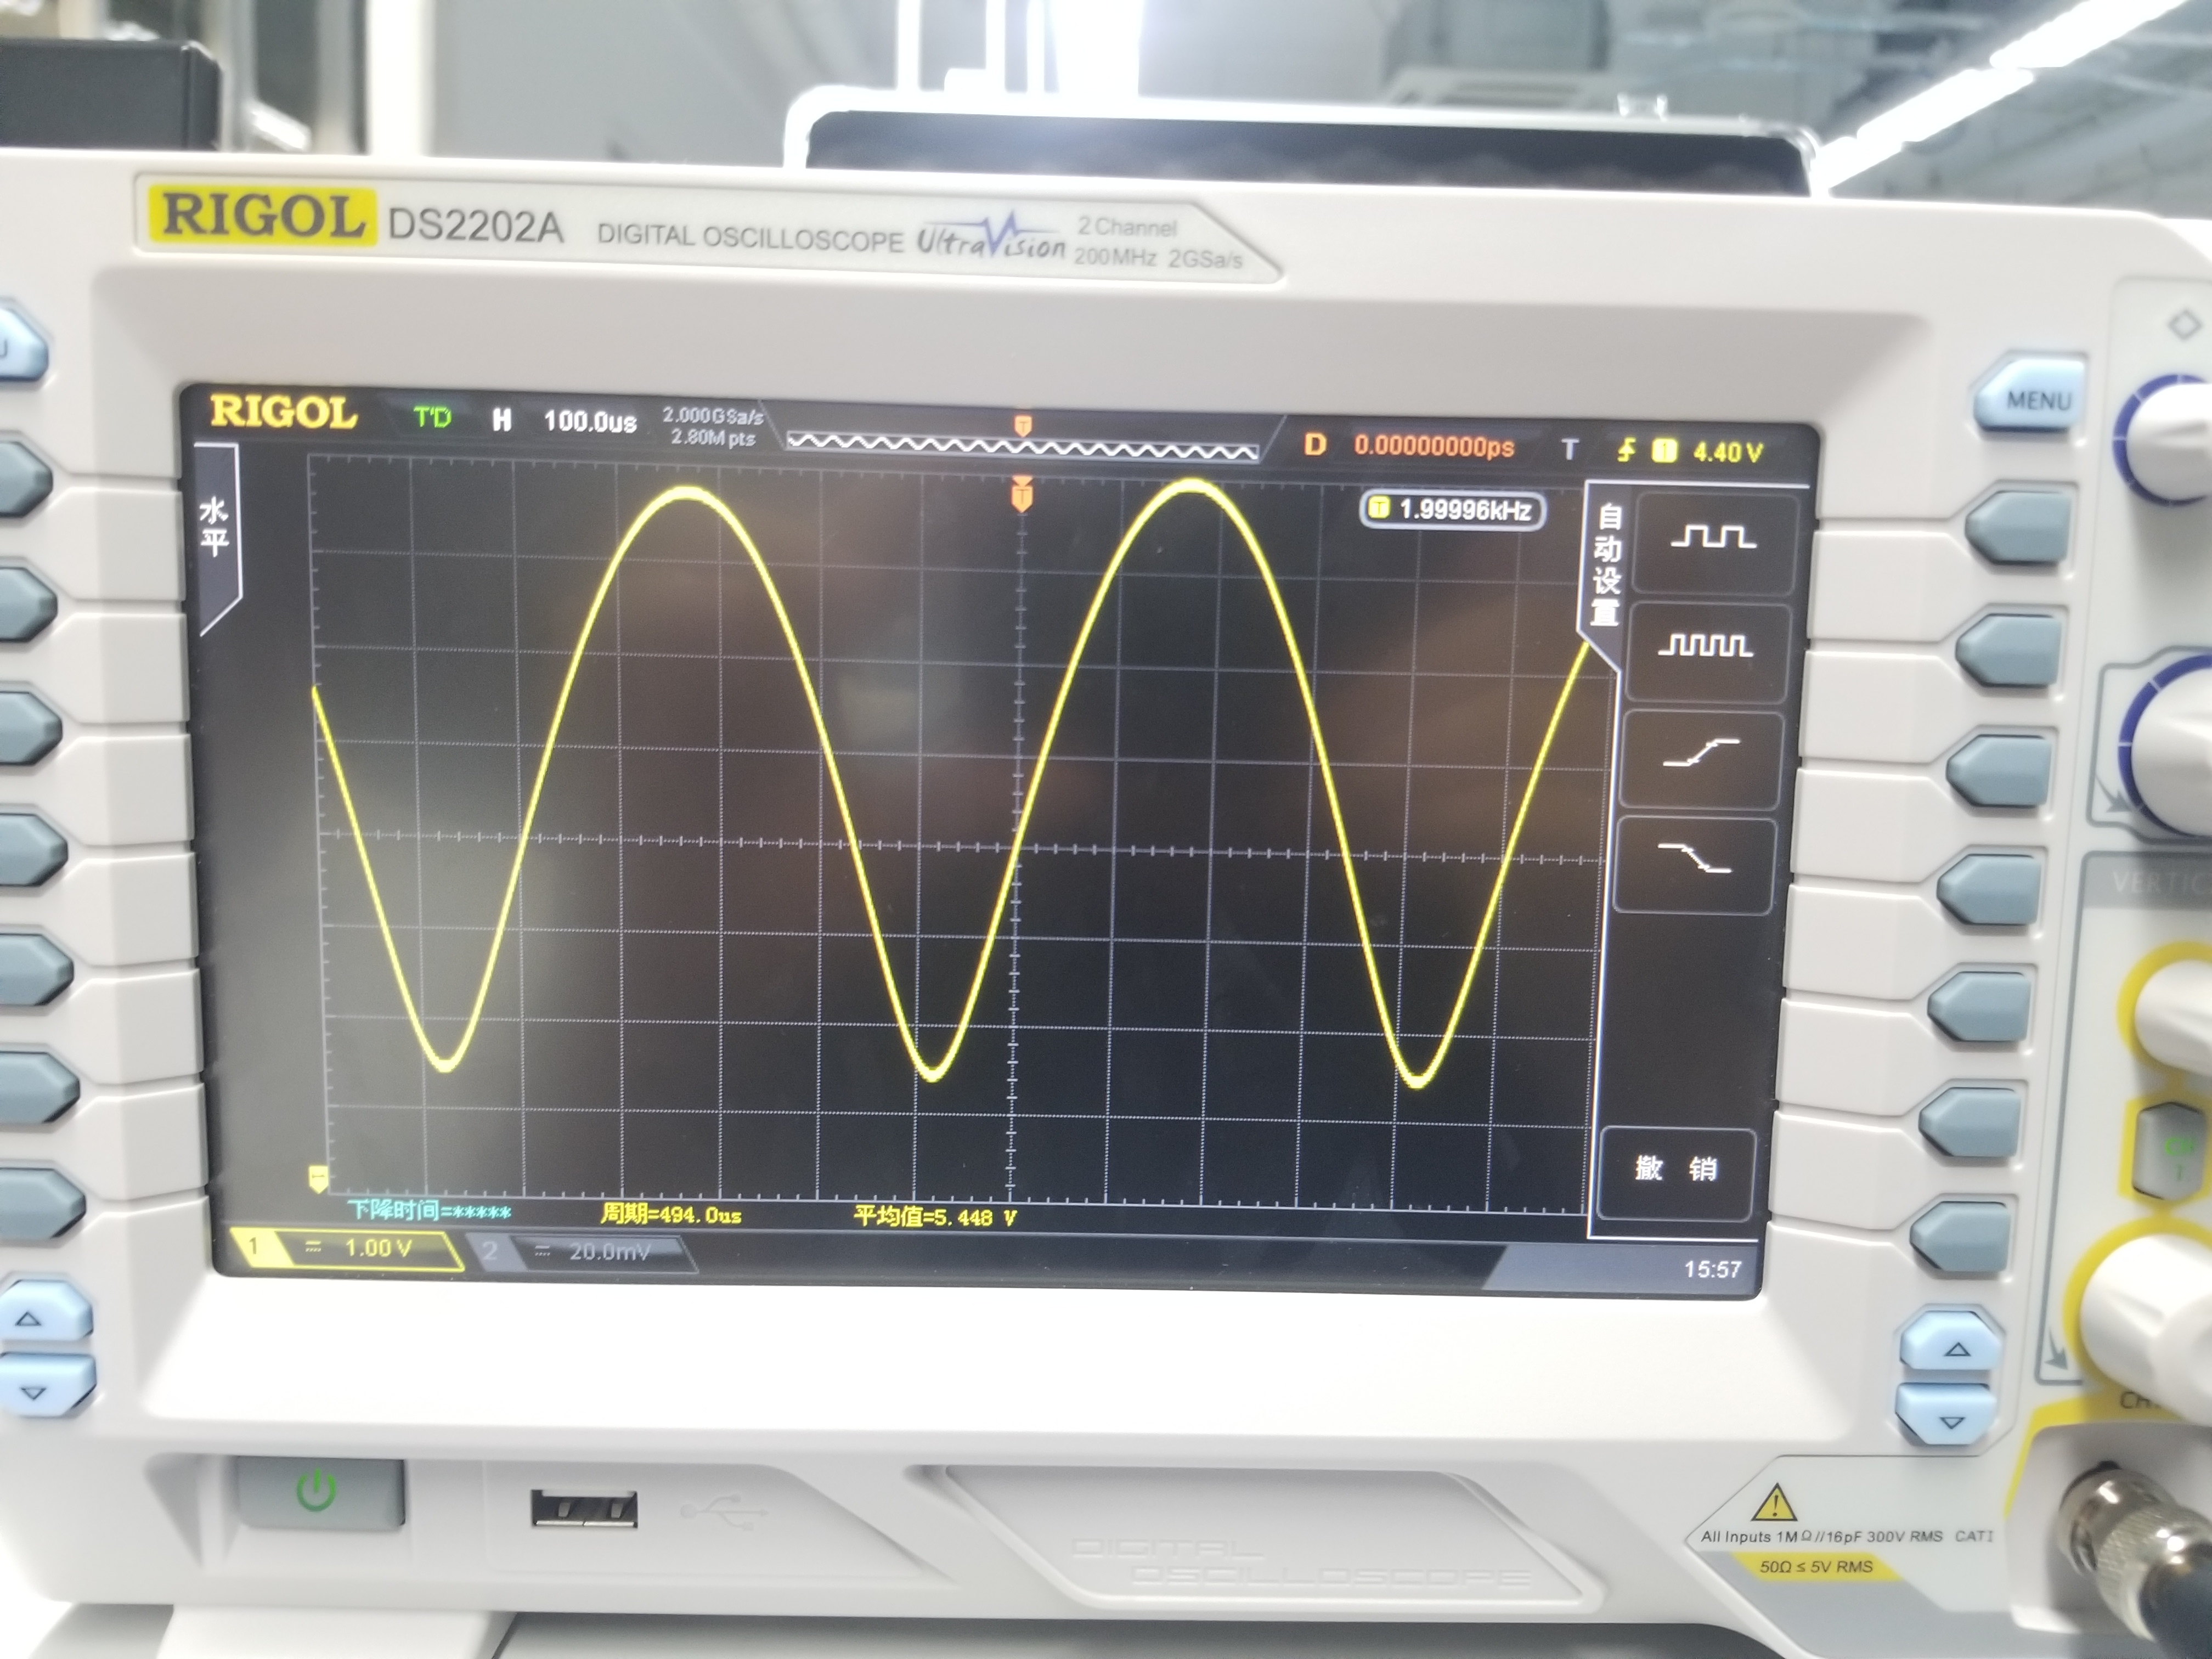
\includegraphics[width=1.5in]{shuju/1/6db_100us_R}}\quad
        \subfloat{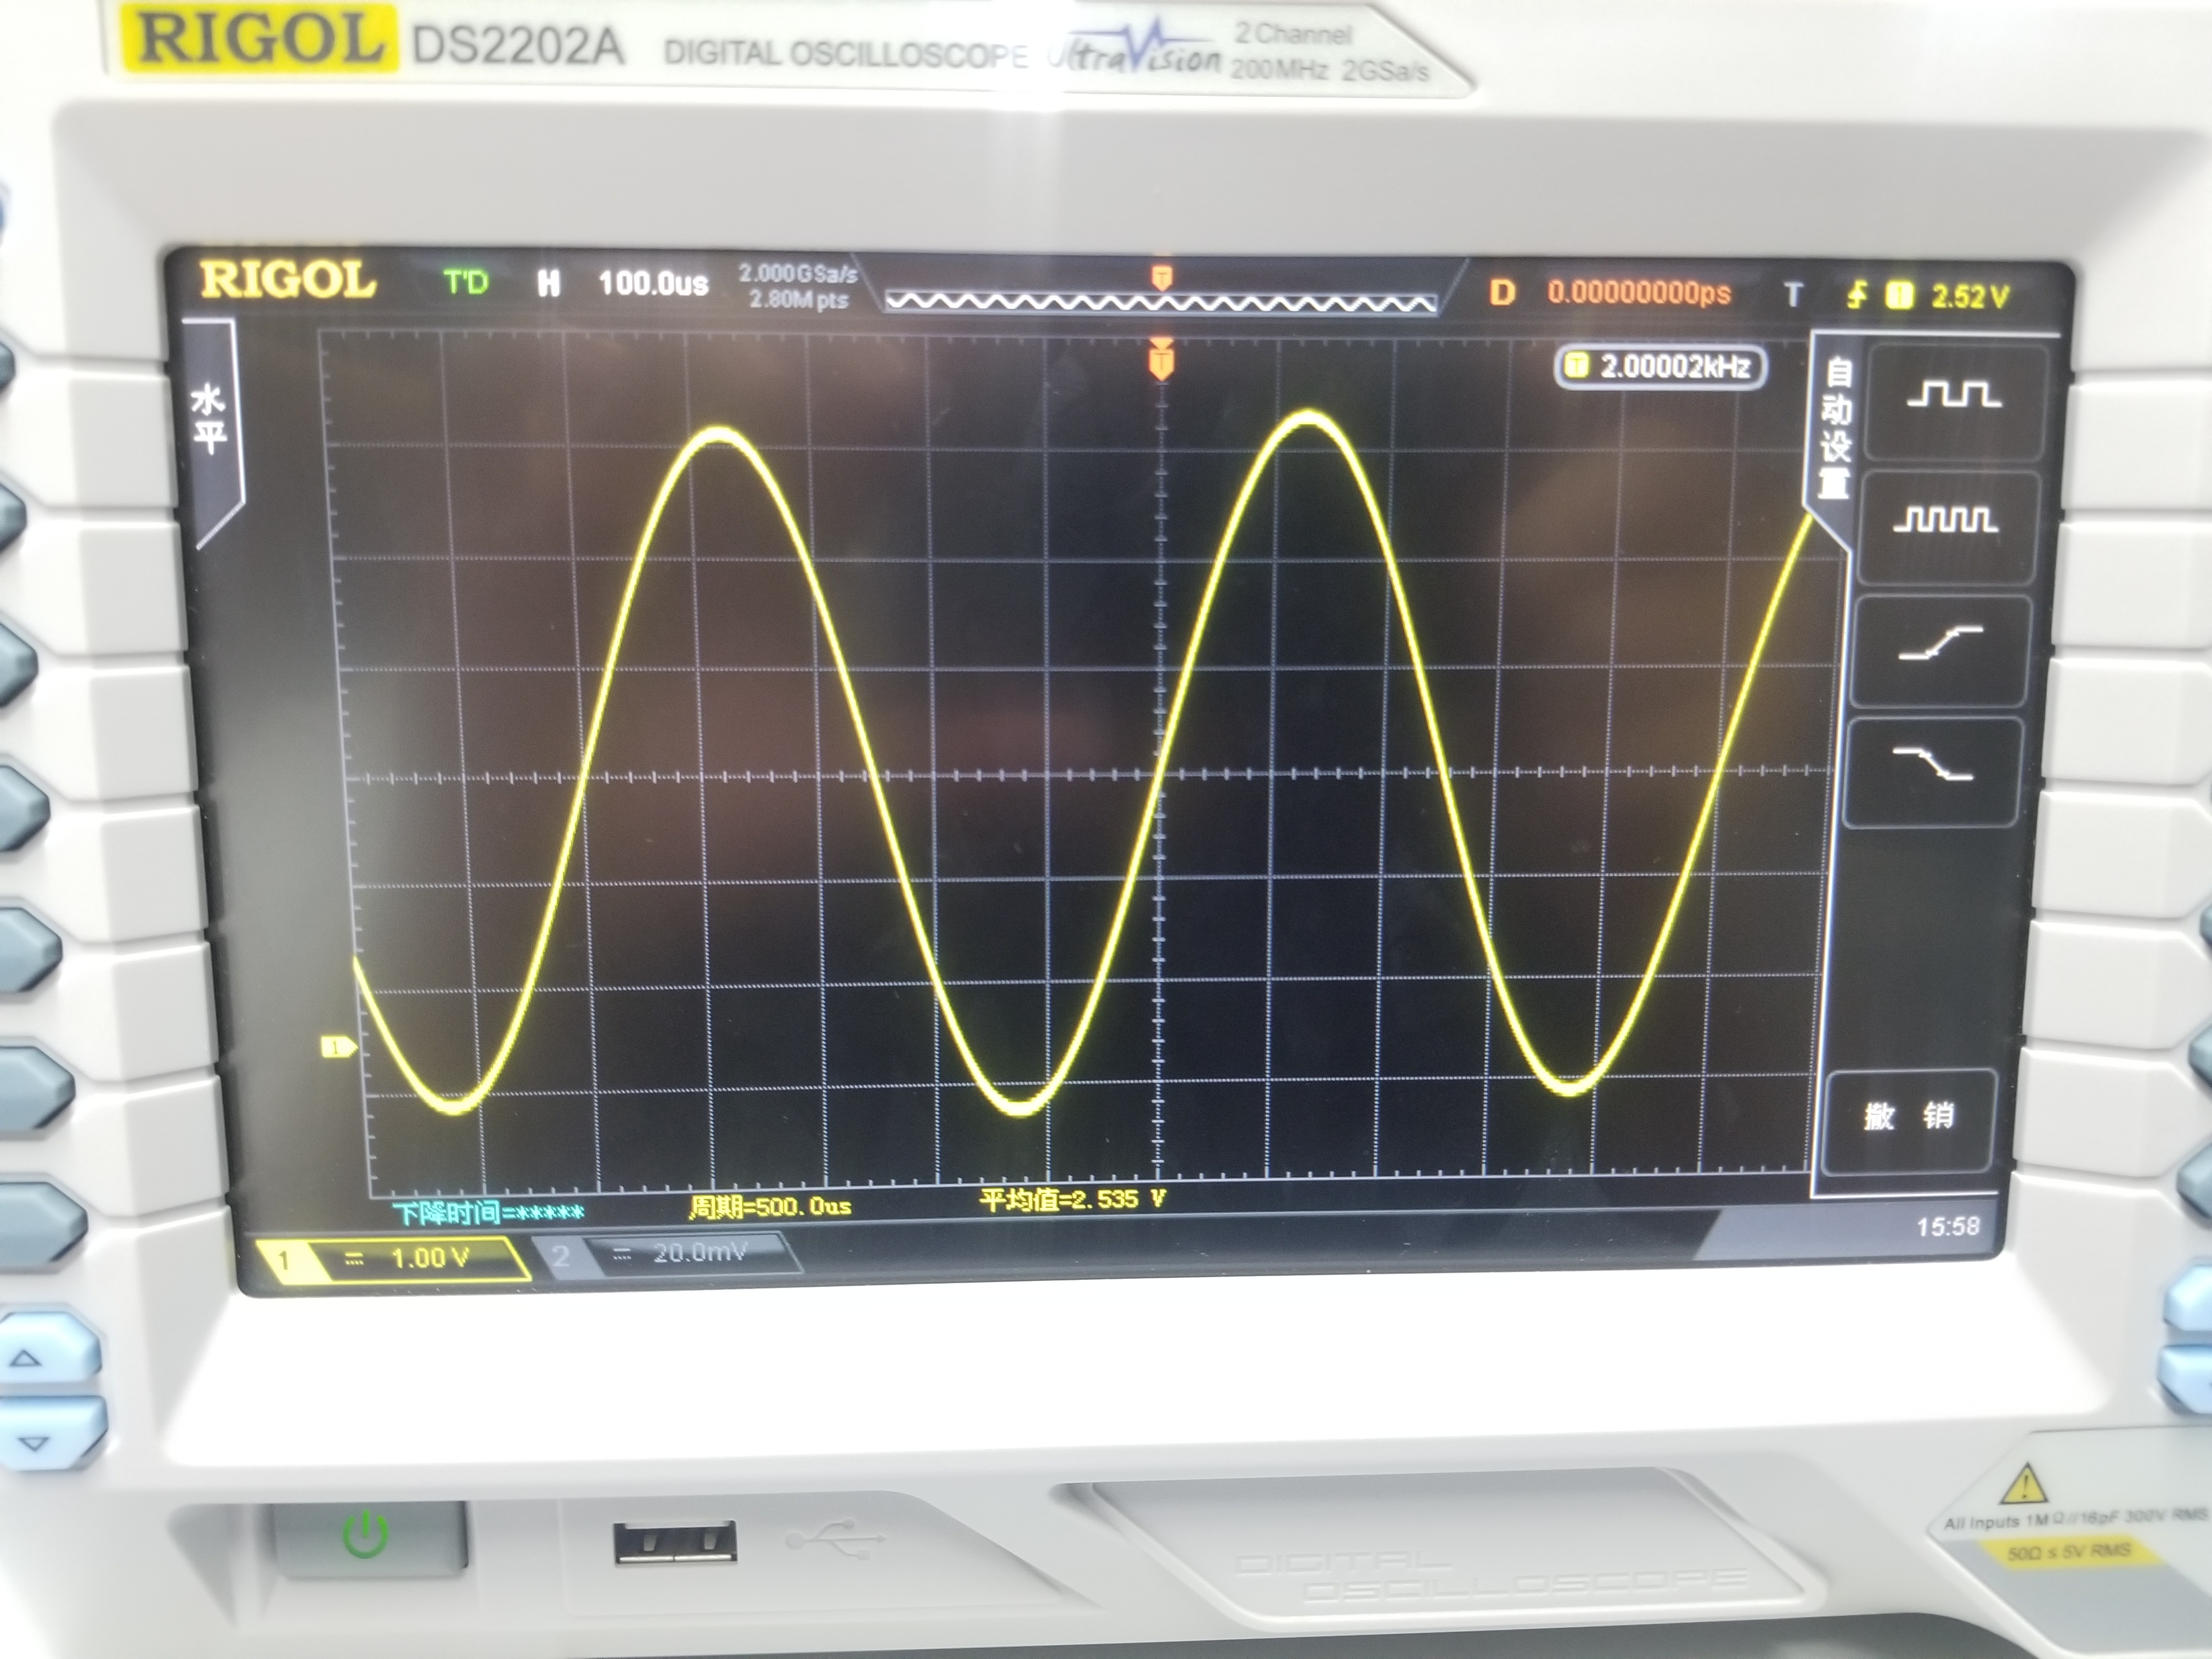
\includegraphics[width=1.5in]{shuju/1/6db_100us_x}}\quad
	\subfloat{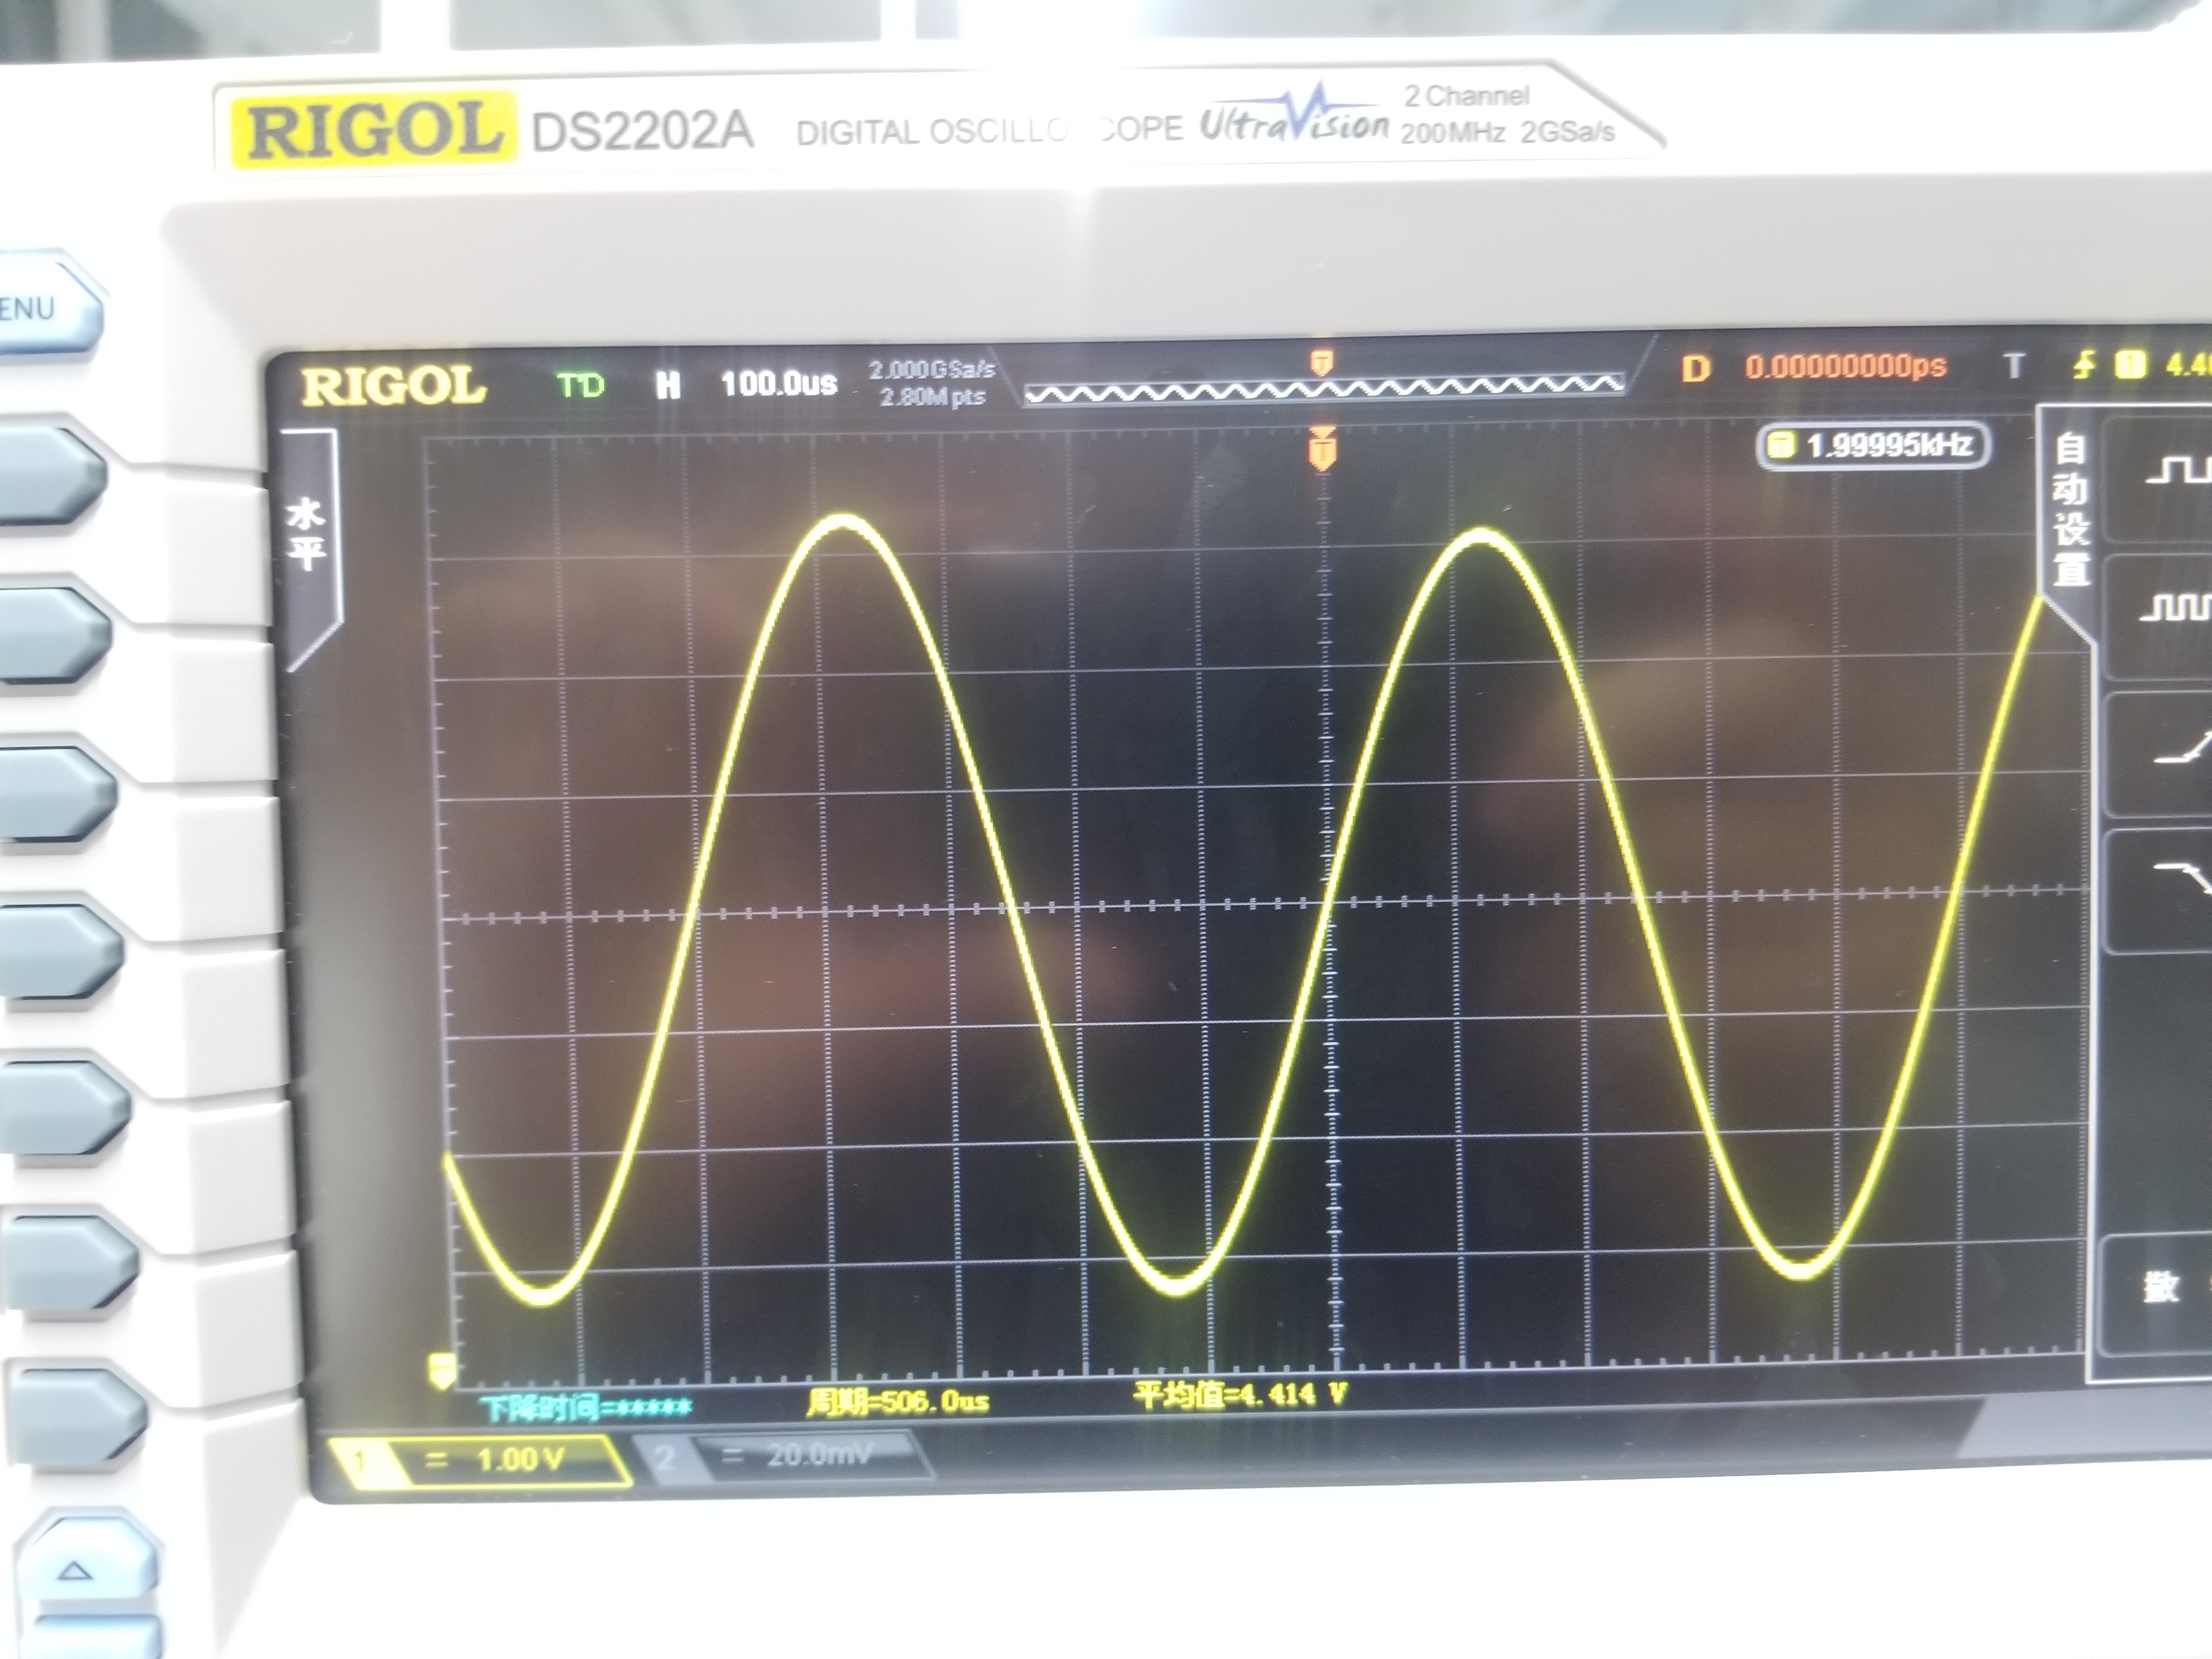
\includegraphics[width=1.5in]{shuju/1/6db_100us_y}}\\	
	\caption{陡降设置为$6dB$,时间常数设置为$100\mathrm{\mu s}$时示波器上的波形,从左边到右边依次为$X,Y,R$的波形。}
\end{figure}
\begin{figure}[H]
	\centering
	\subfloat{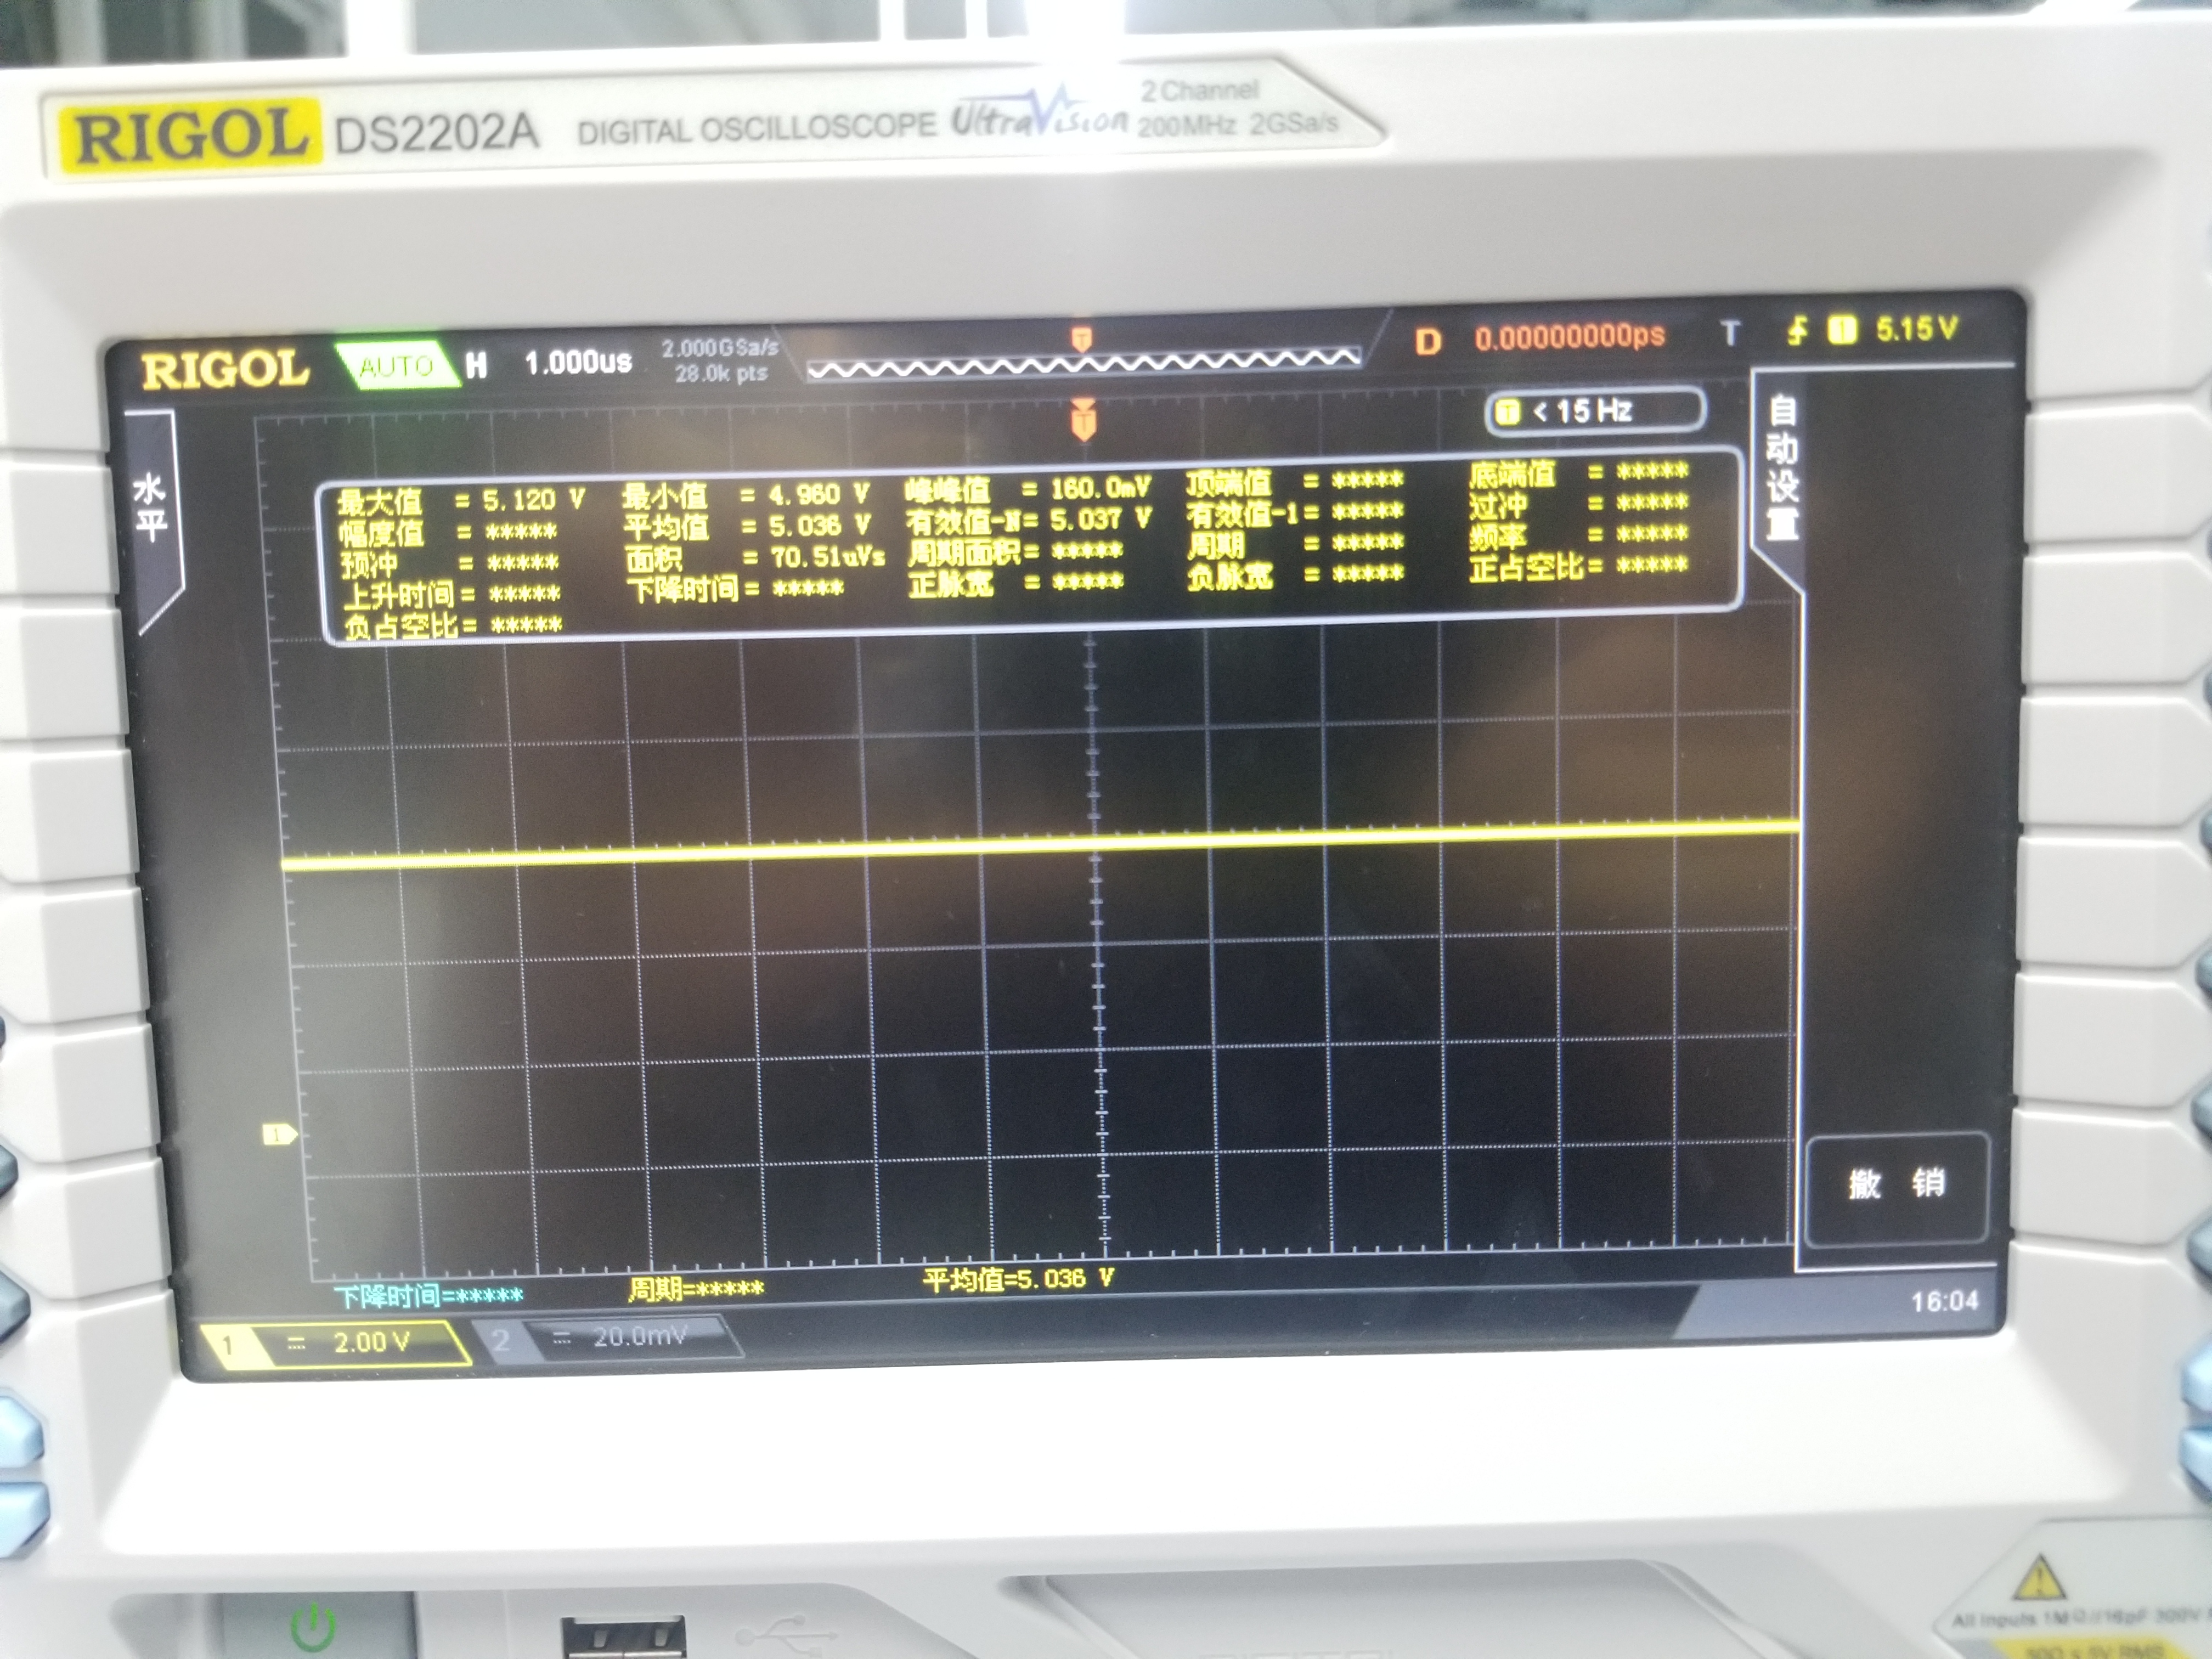
\includegraphics[width=1.5in]{shuju/1/6db_300ms_R}}\quad
        \subfloat{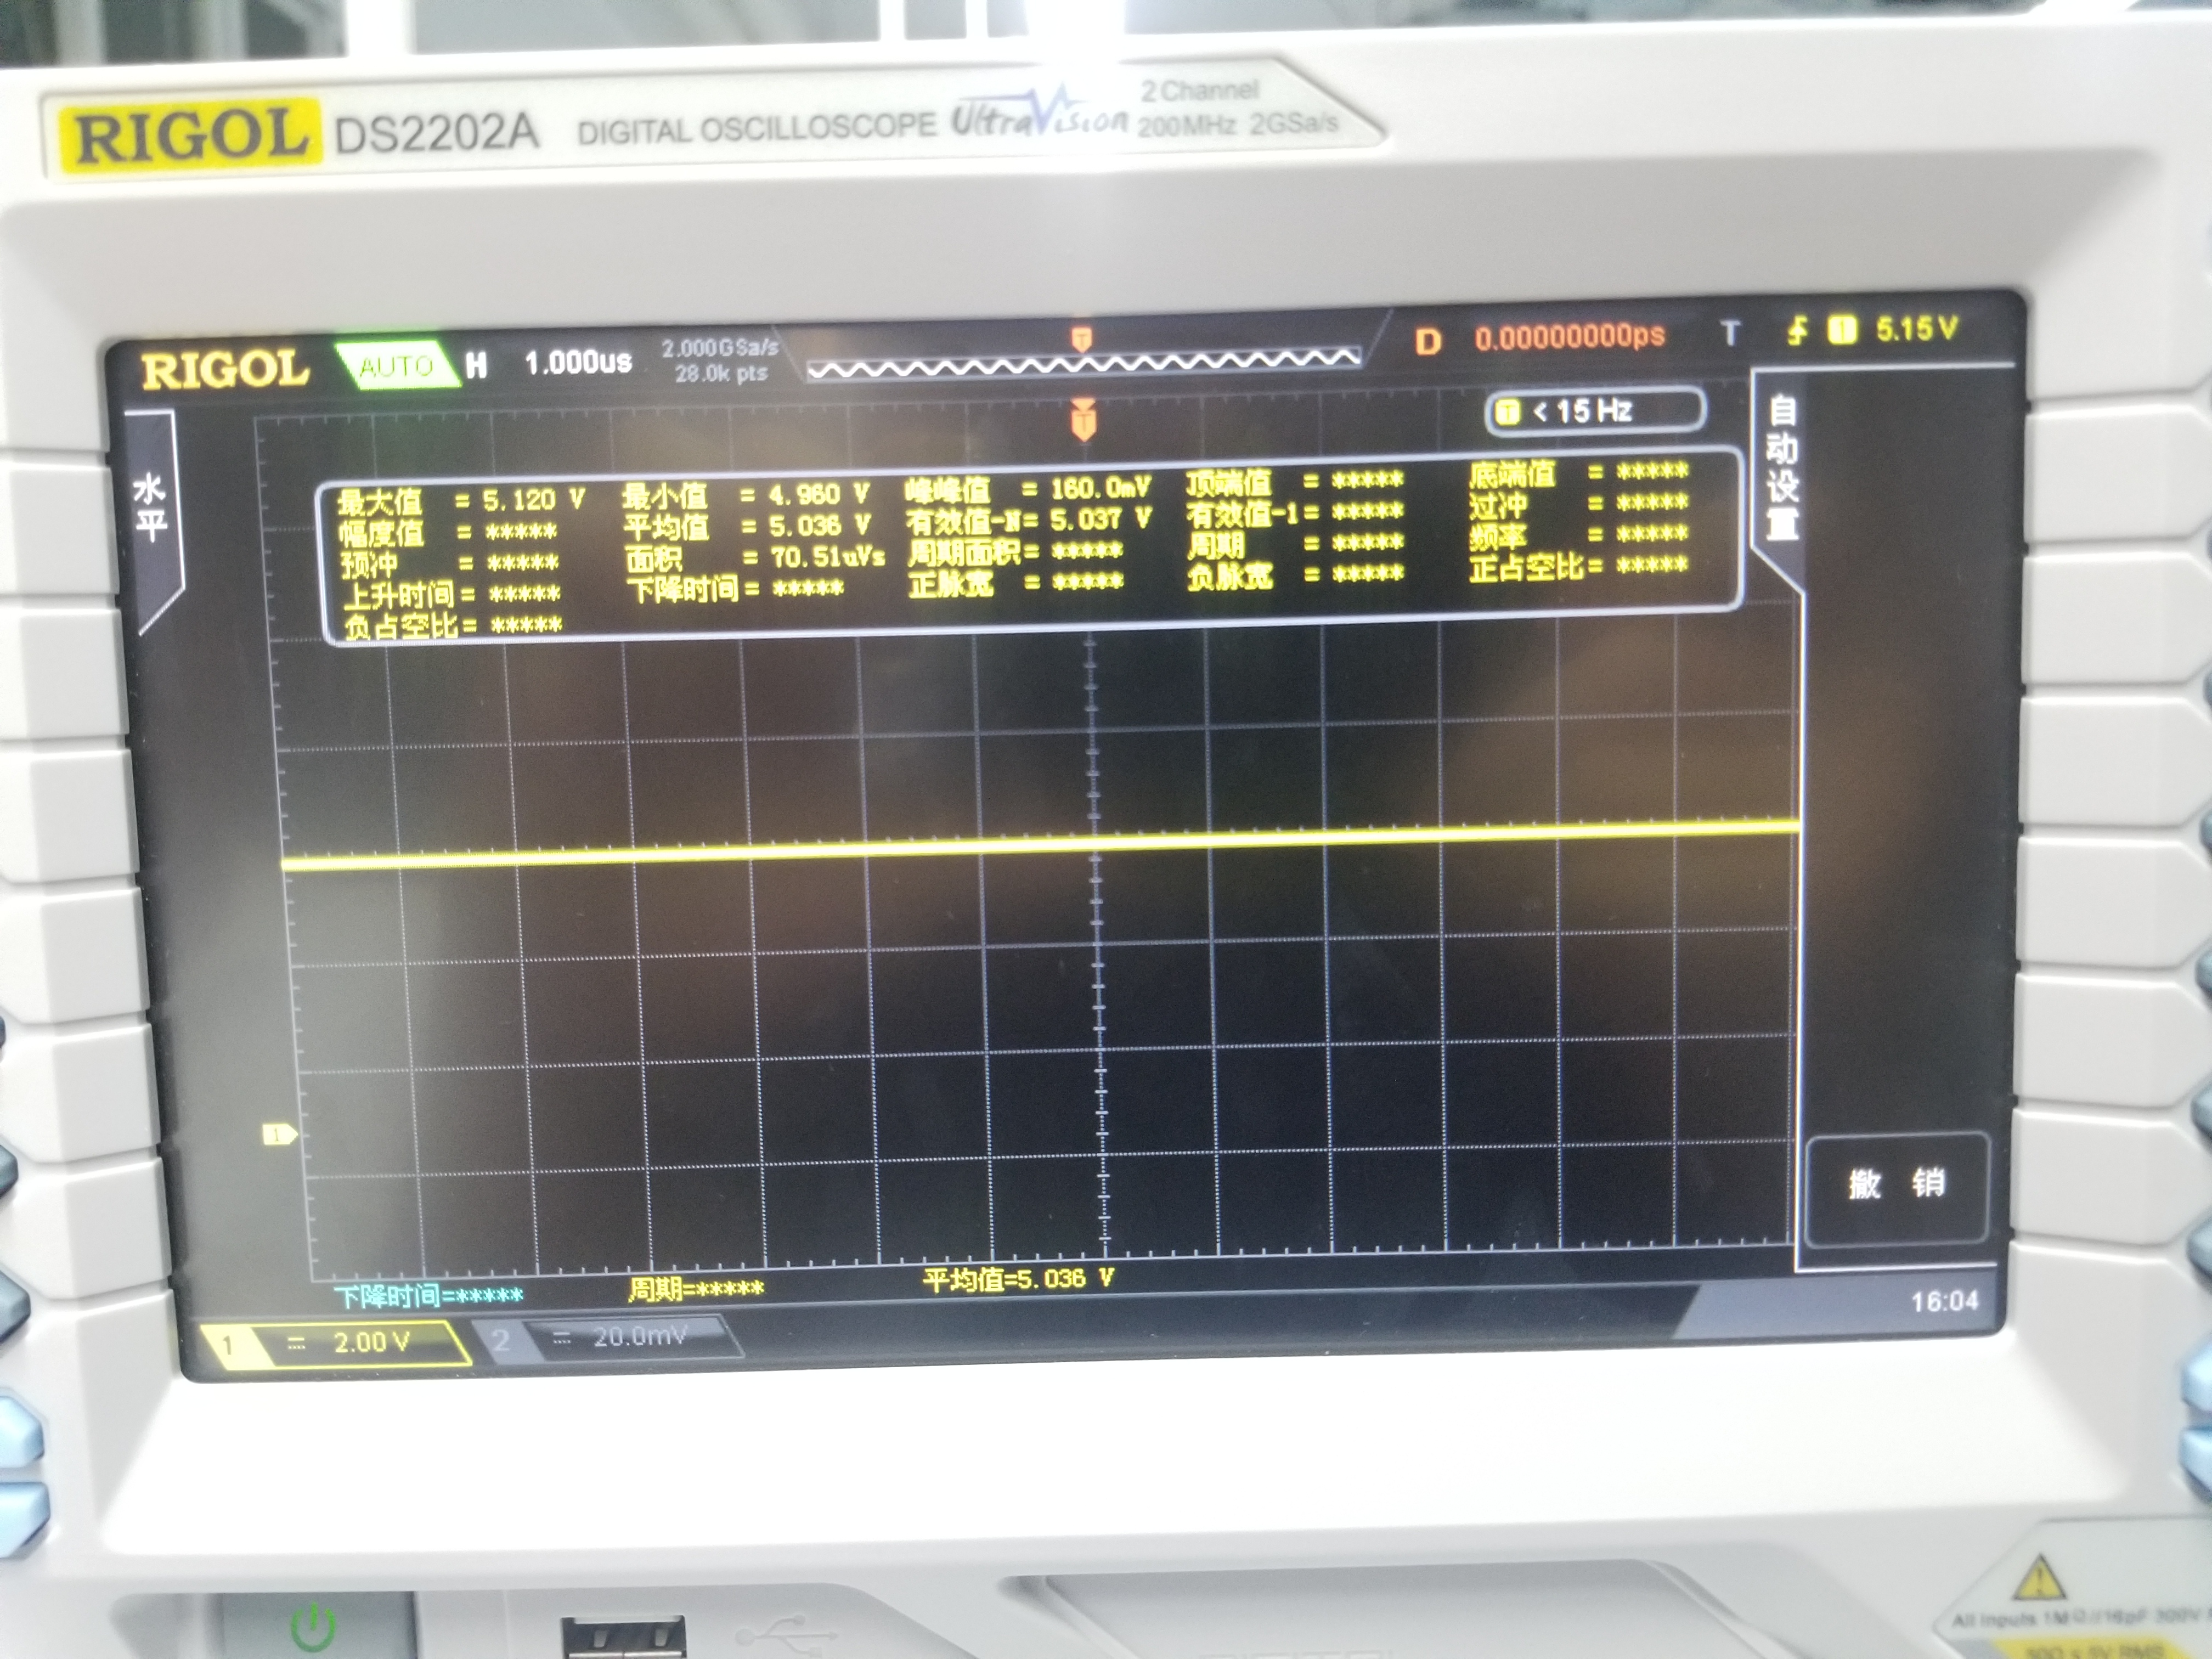
\includegraphics[width=1.5in]{shuju/1/6db_300ms_R}}\quad
	\subfloat{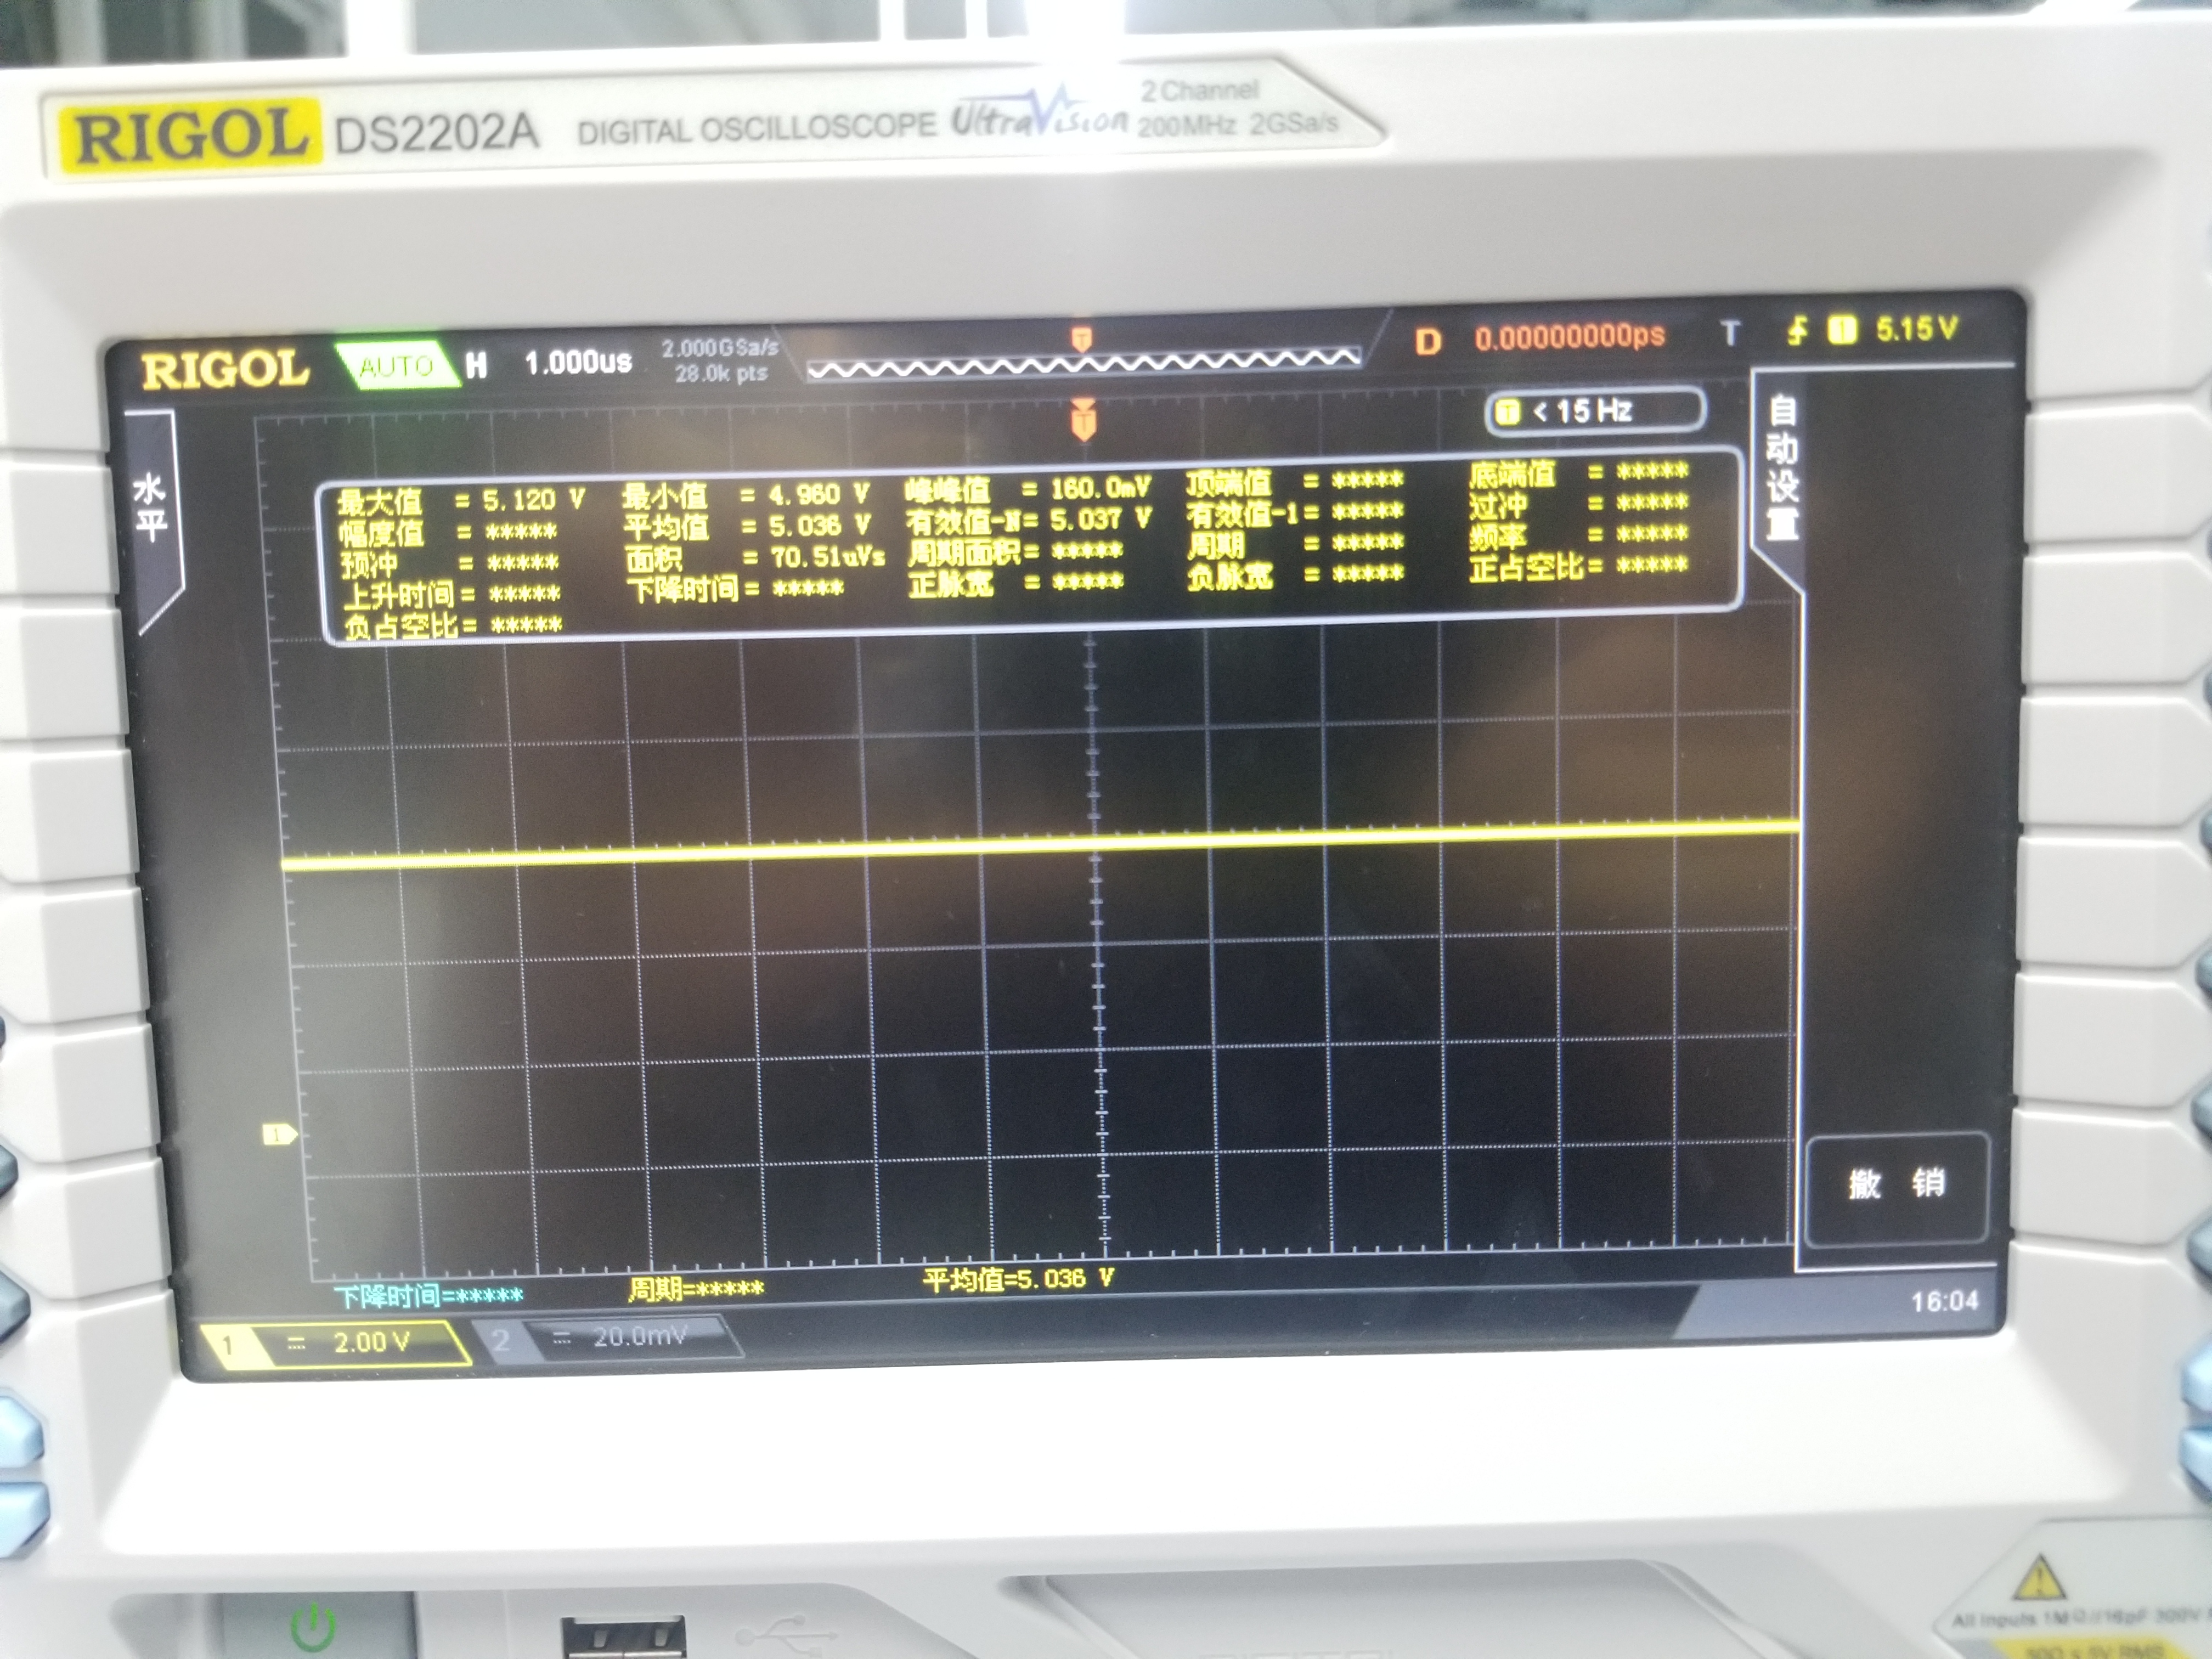
\includegraphics[width=1.5in]{shuju/1/6db_300ms_R}}\\	
	\caption{陡降设置为$6dB$,时间常数设置为$300\mathrm{ms}$时示波器上的波形,从左边到右边依次为$X,Y,R$的波形。}
\end{figure}
由上面的一系列波形,我们可以理解时间常数对于锁相放大器的作用:时间常数是低通滤波器$RC$电路的时间常数。可以简单地认为,时间常数越大,阶数越高,输出的带宽就越低,显示的测量幅度、相位等值就越稳定。然而,过大的时间常数会抹平输入信号(随时间)的变化,从而失去有用的信息。因此,在实际应用中,需要根据输入信号随时间变化的情况,协调时间常数与信噪比之间的平衡。在实验中,我们观察到,如果时间常数很大,则抹平了信号随时间的变化,当时间常数大约为{\color{red} $300$倍信号周期}时,完全抹平了信号中有用的信息,从而变为单调的直流输出。

\item 我们现在固定时间常数,改变陡降,探究陡降对于波形的影响。
\begin{figure}[H]
	\centering
	\subfloat{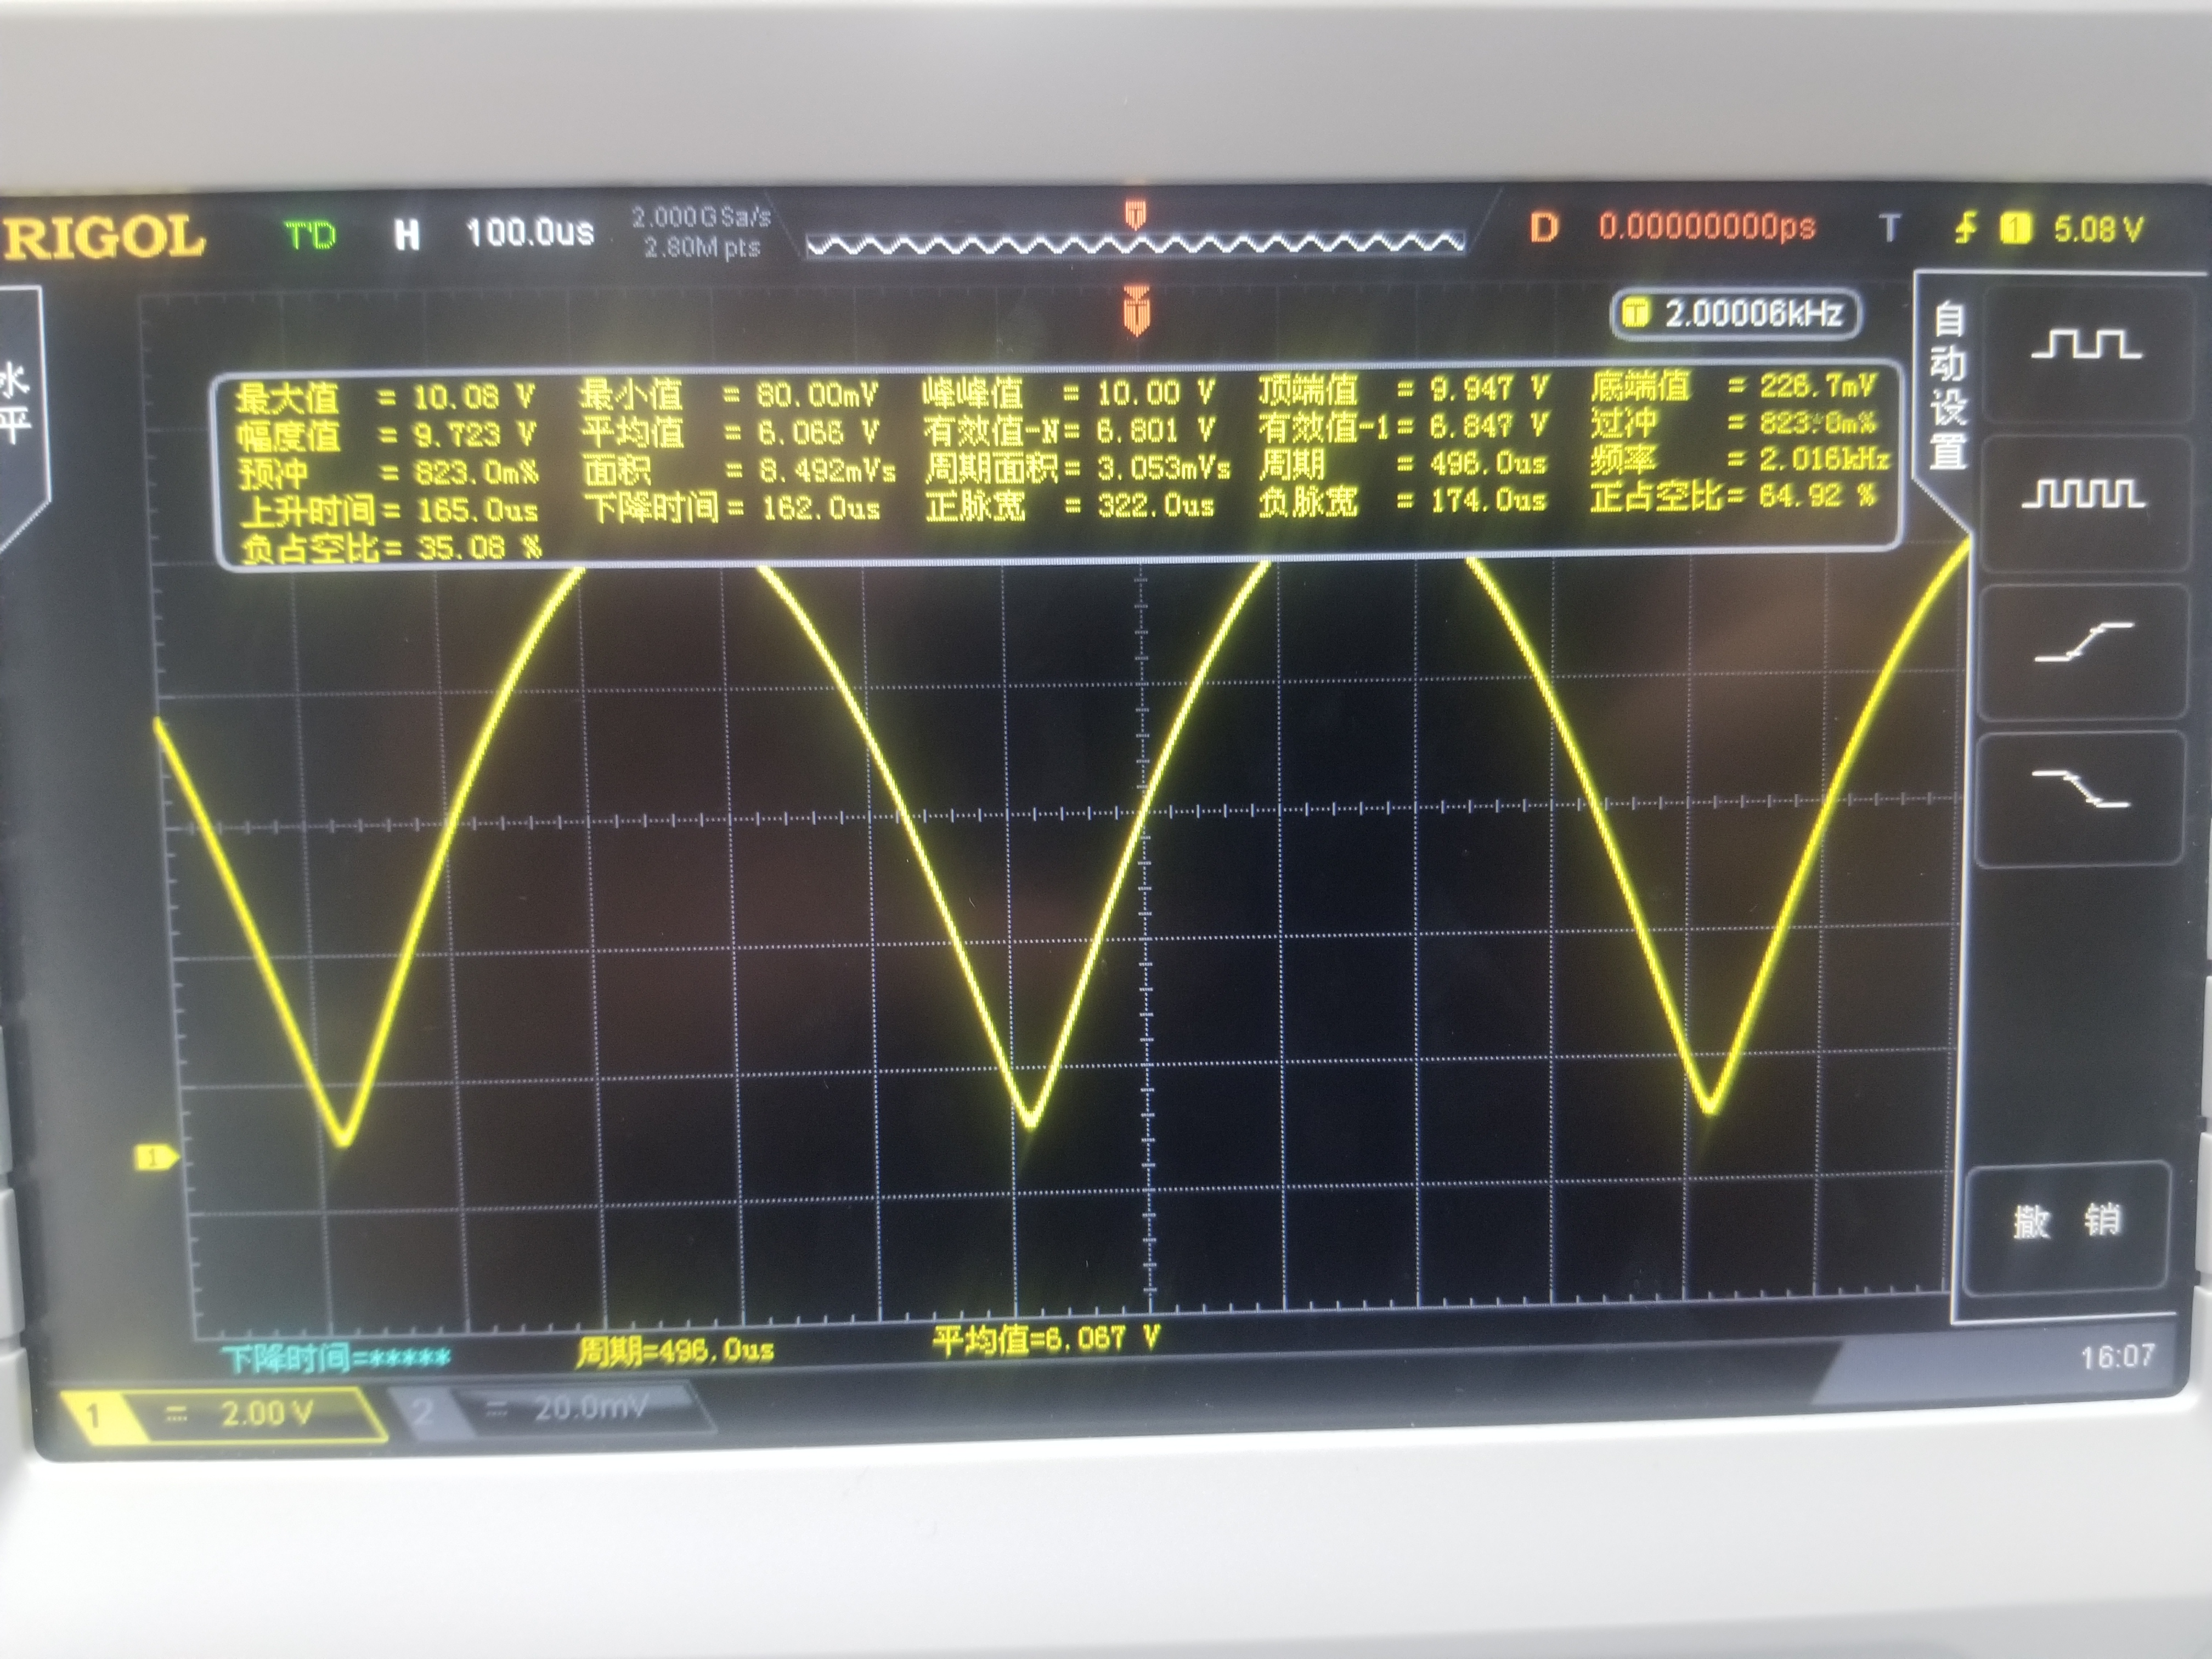
\includegraphics[width=1.5in]{shuju/2/6db_30us_R}}\quad
        \subfloat{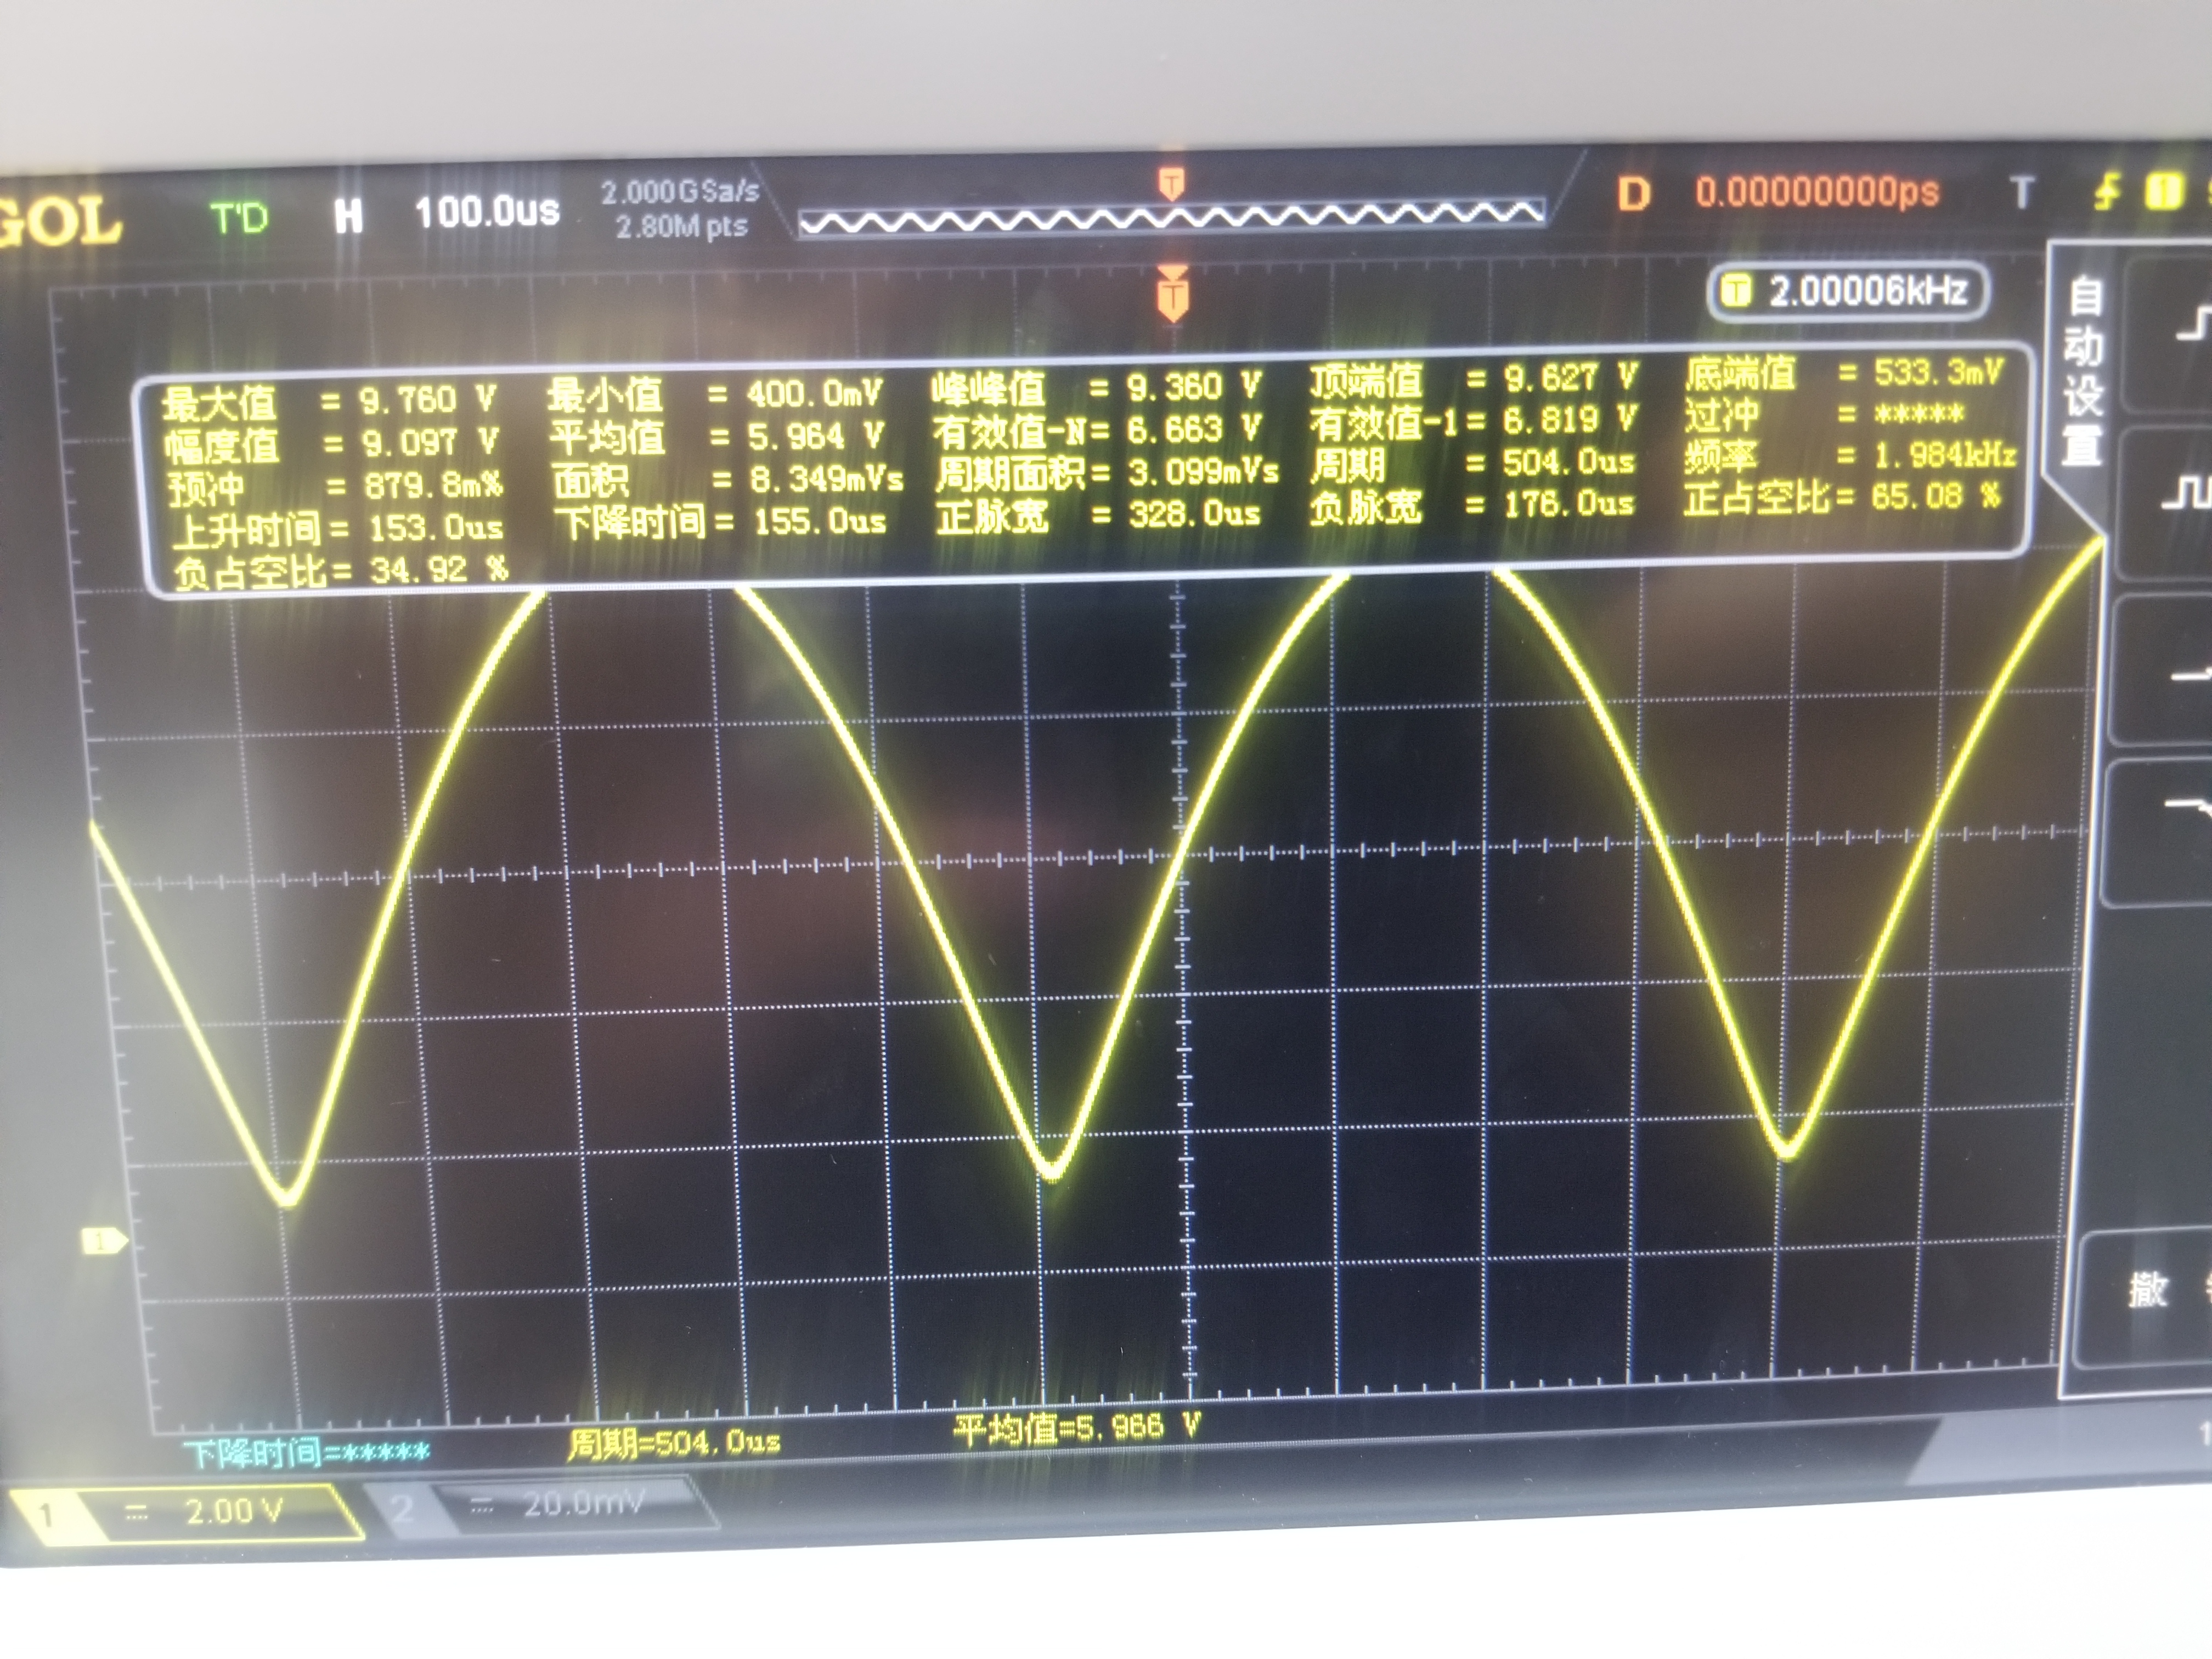
\includegraphics[width=1.5in]{shuju/2/12db_30us_R}}\quad
	\subfloat{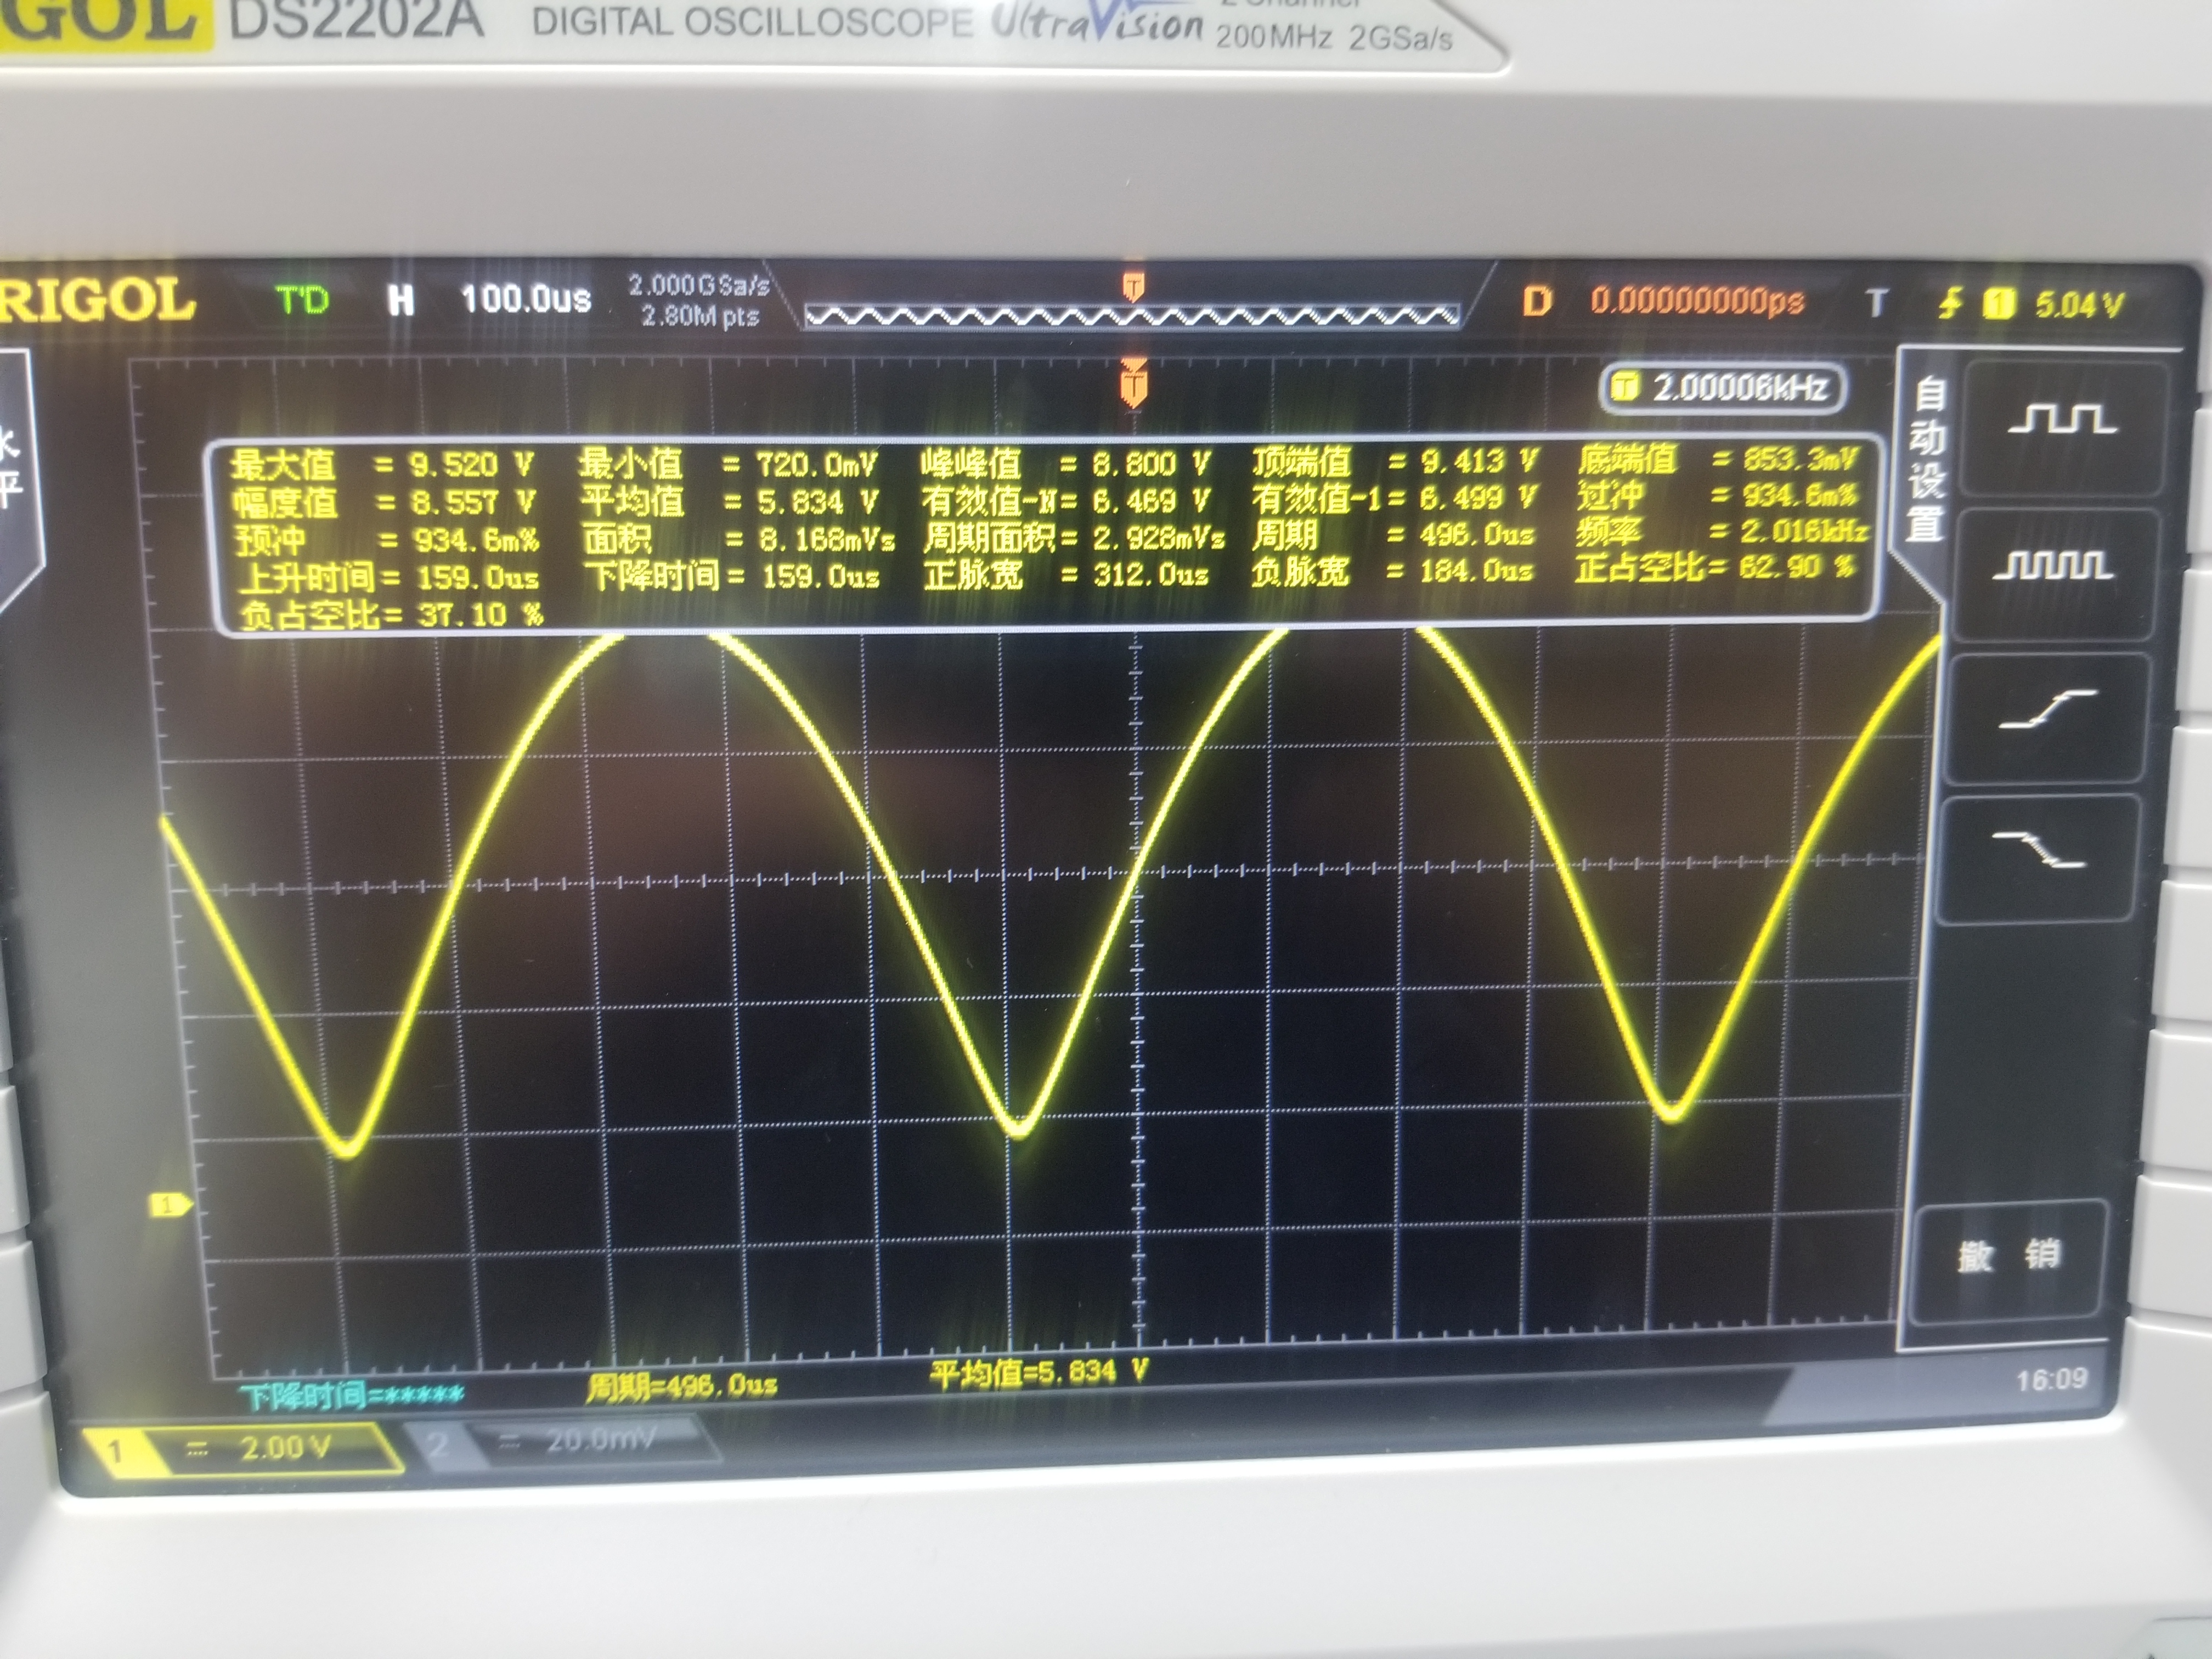
\includegraphics[width=1.5in]{shuju/2/18db_30us_R}}\quad
	\subfloat{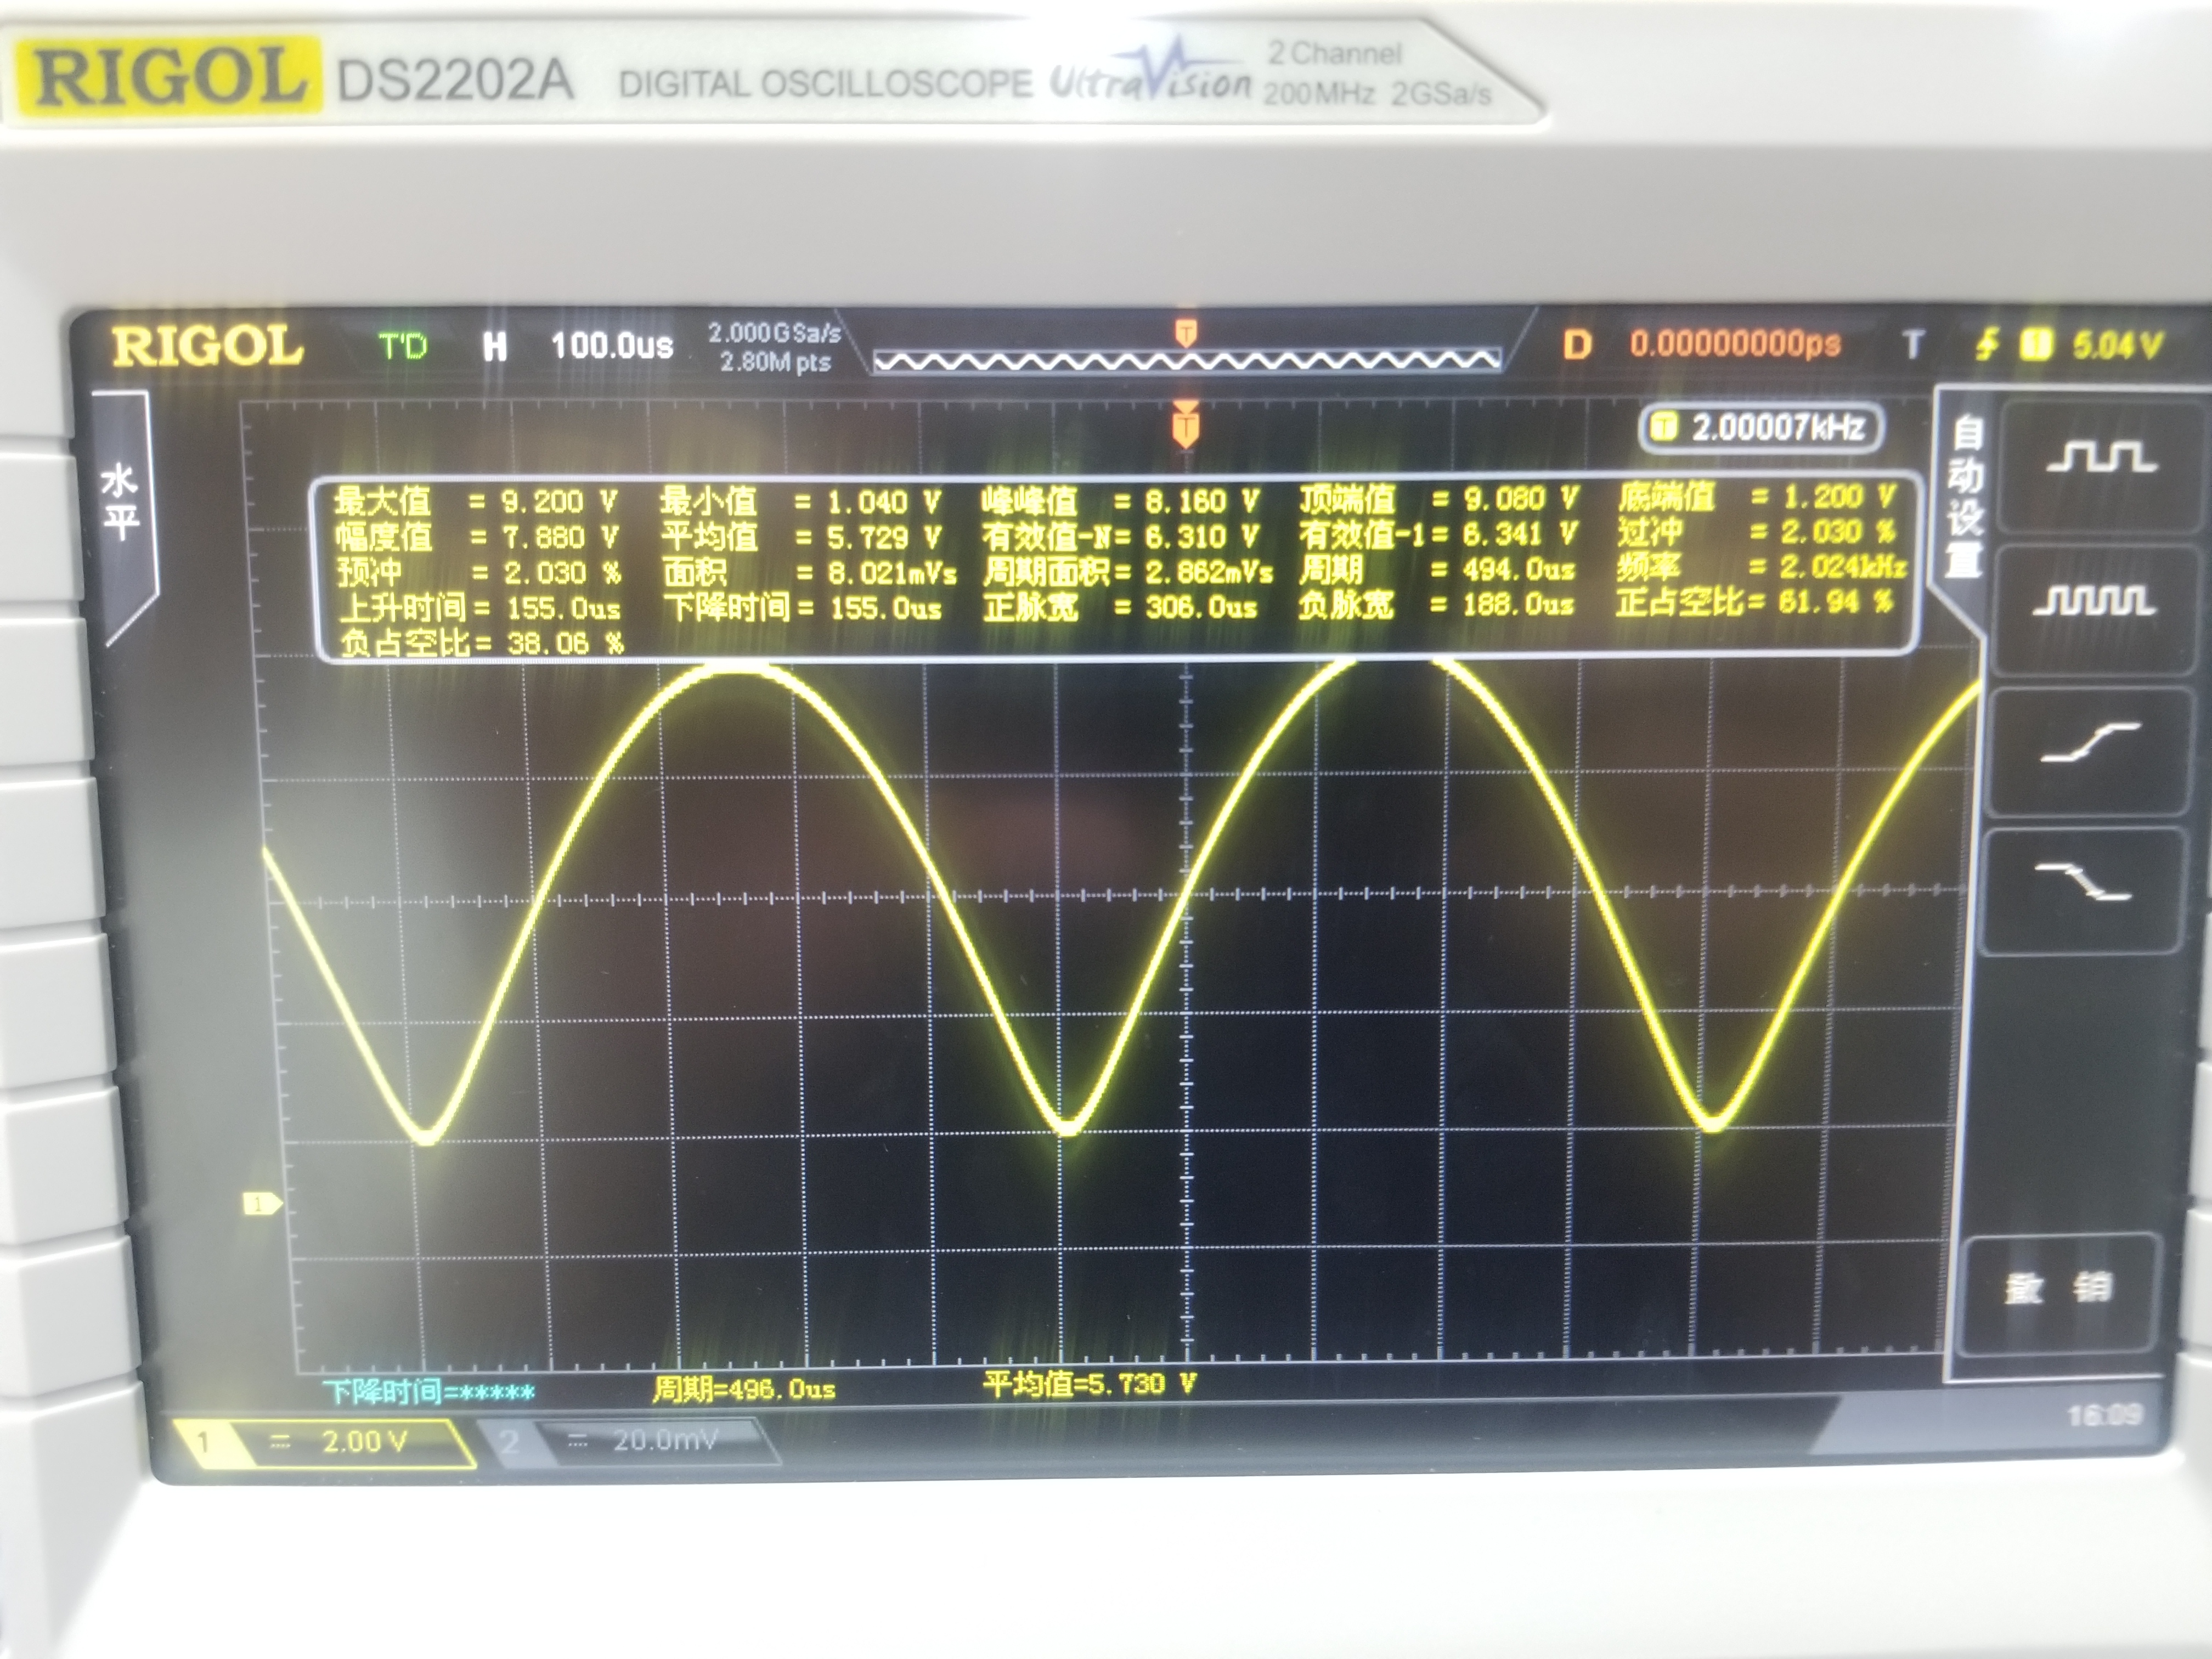
\includegraphics[width=1.5in]{shuju/2/24db_30us_R}}\\
	\caption{陡降设置分别为$6dB,12dB,18dB,24dB$,时间常数固定为$30\mathrm{\mu s}$时示波器上的波形。}
\end{figure}


\begin{figure}[H]
	\centering
	\subfloat{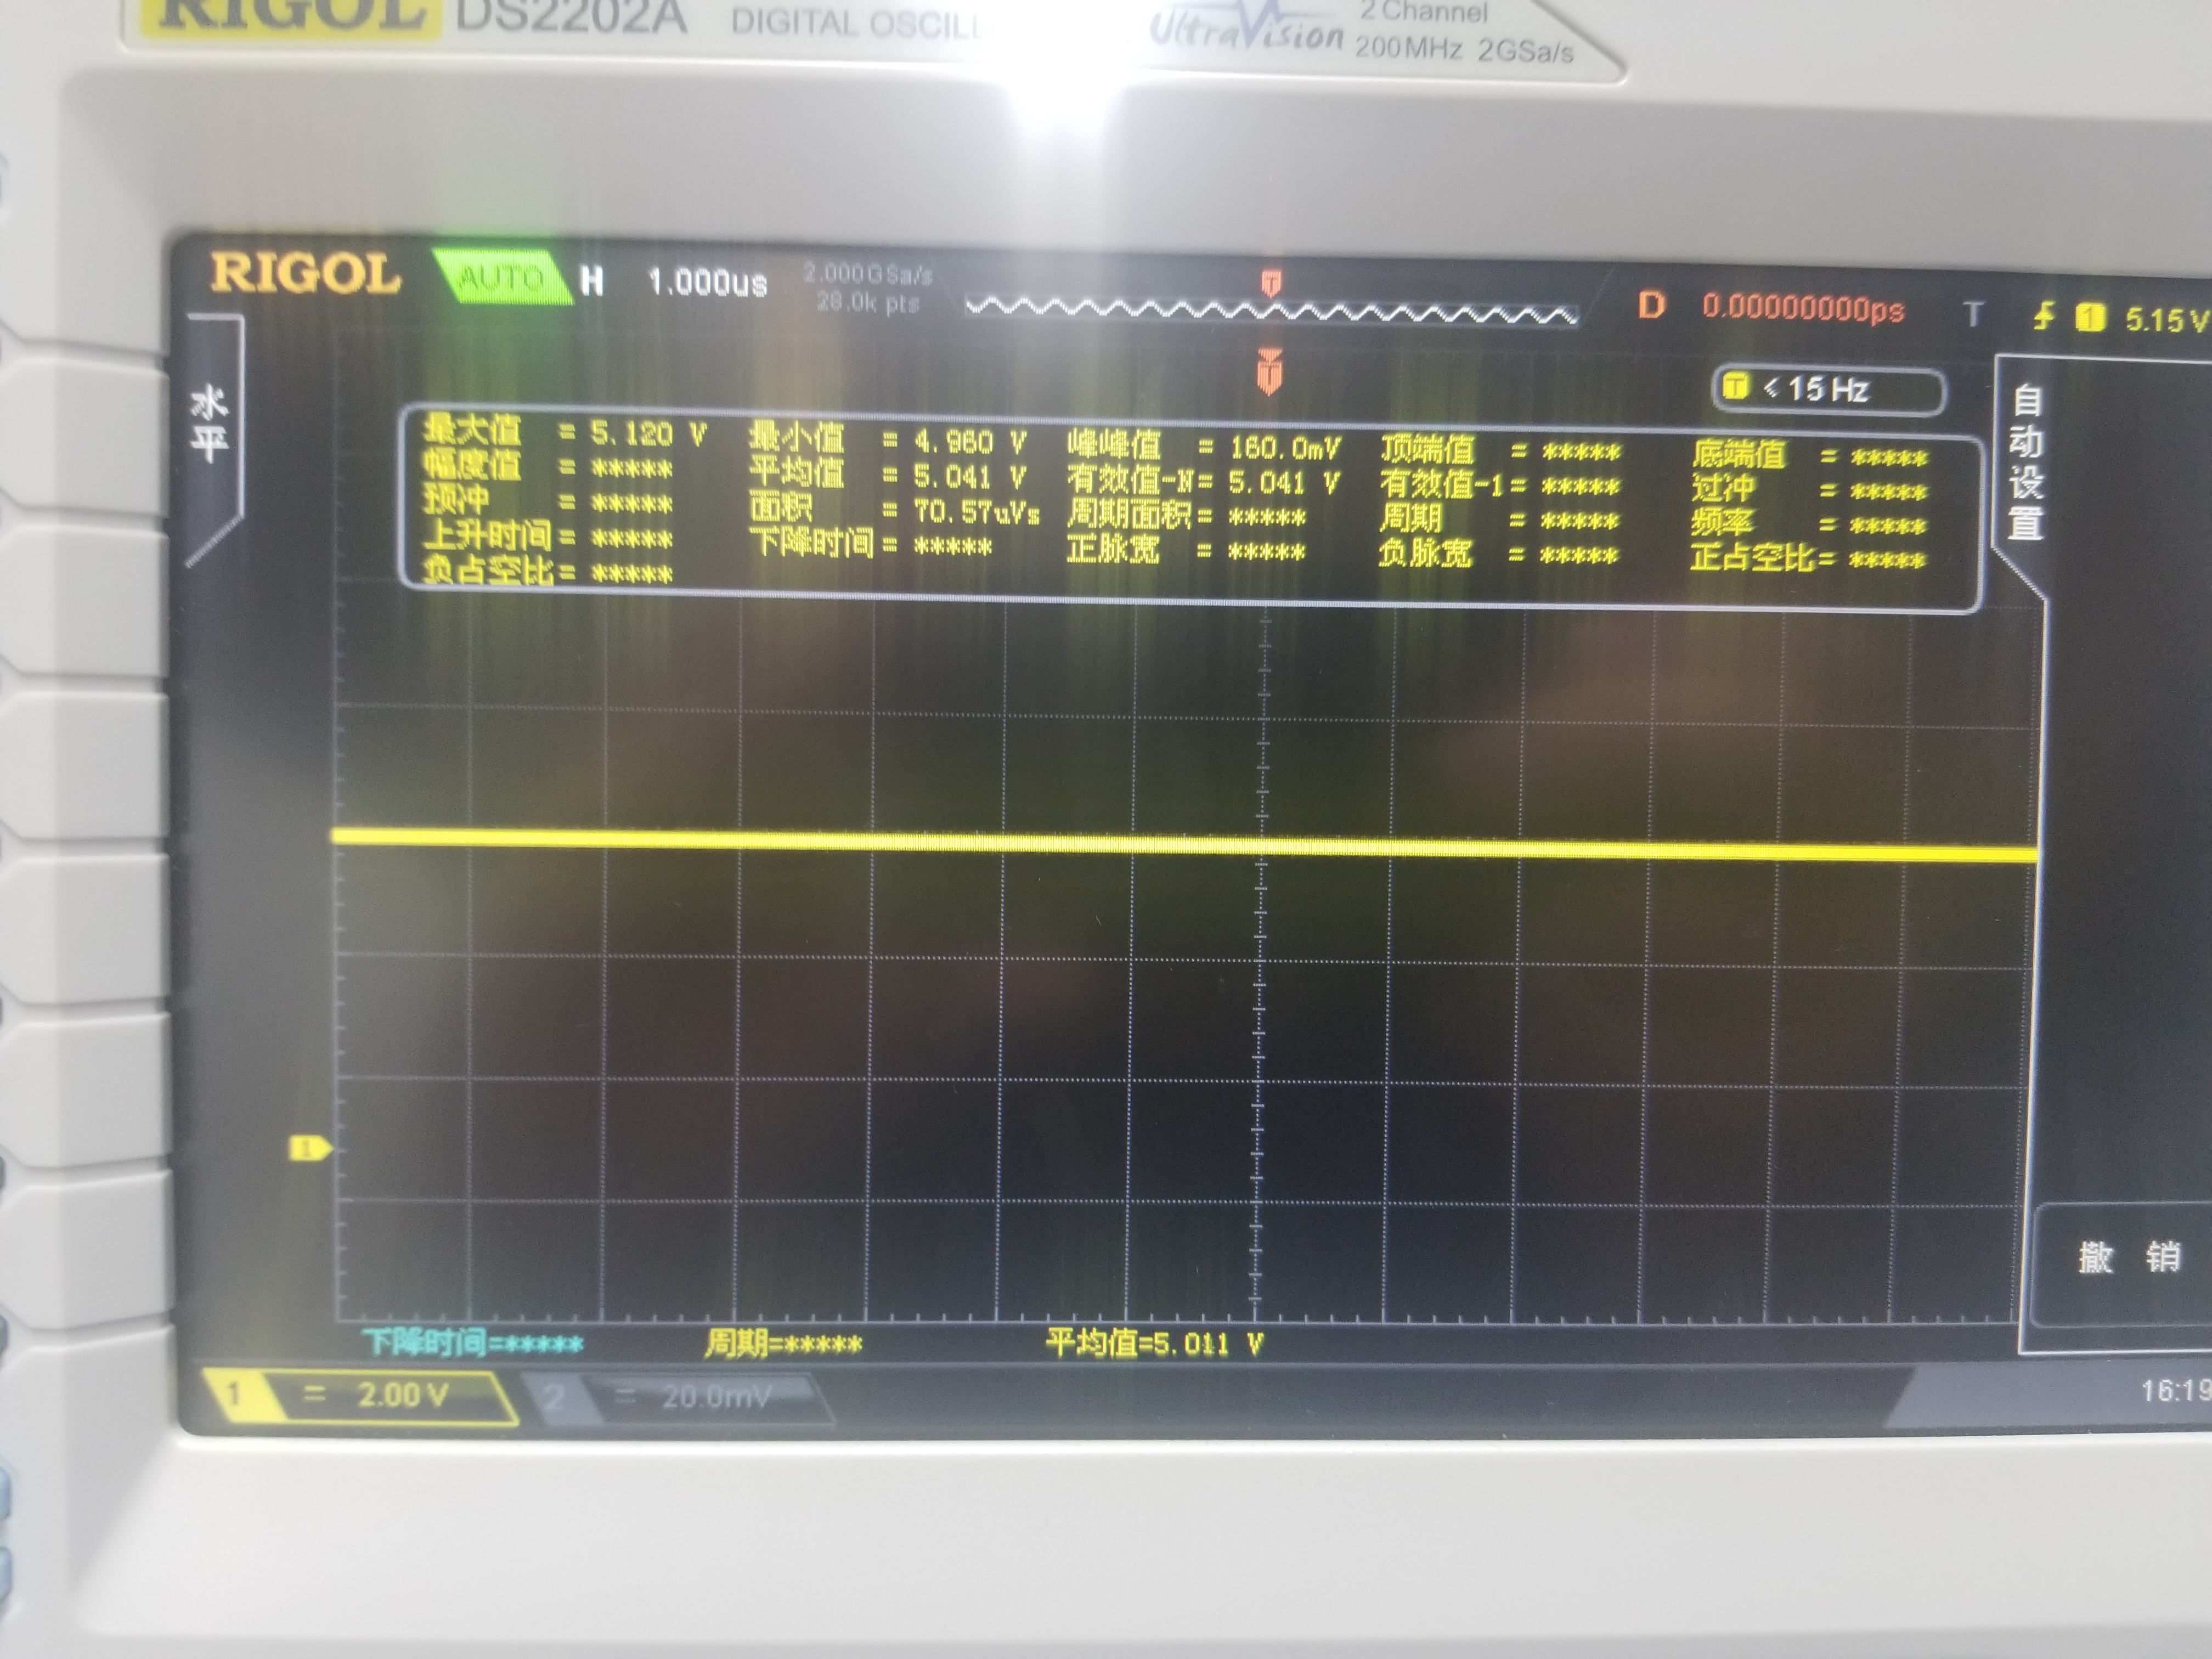
\includegraphics[width=1.5in]{shuju/2/6db_10ms_R}}\quad
	\subfloat{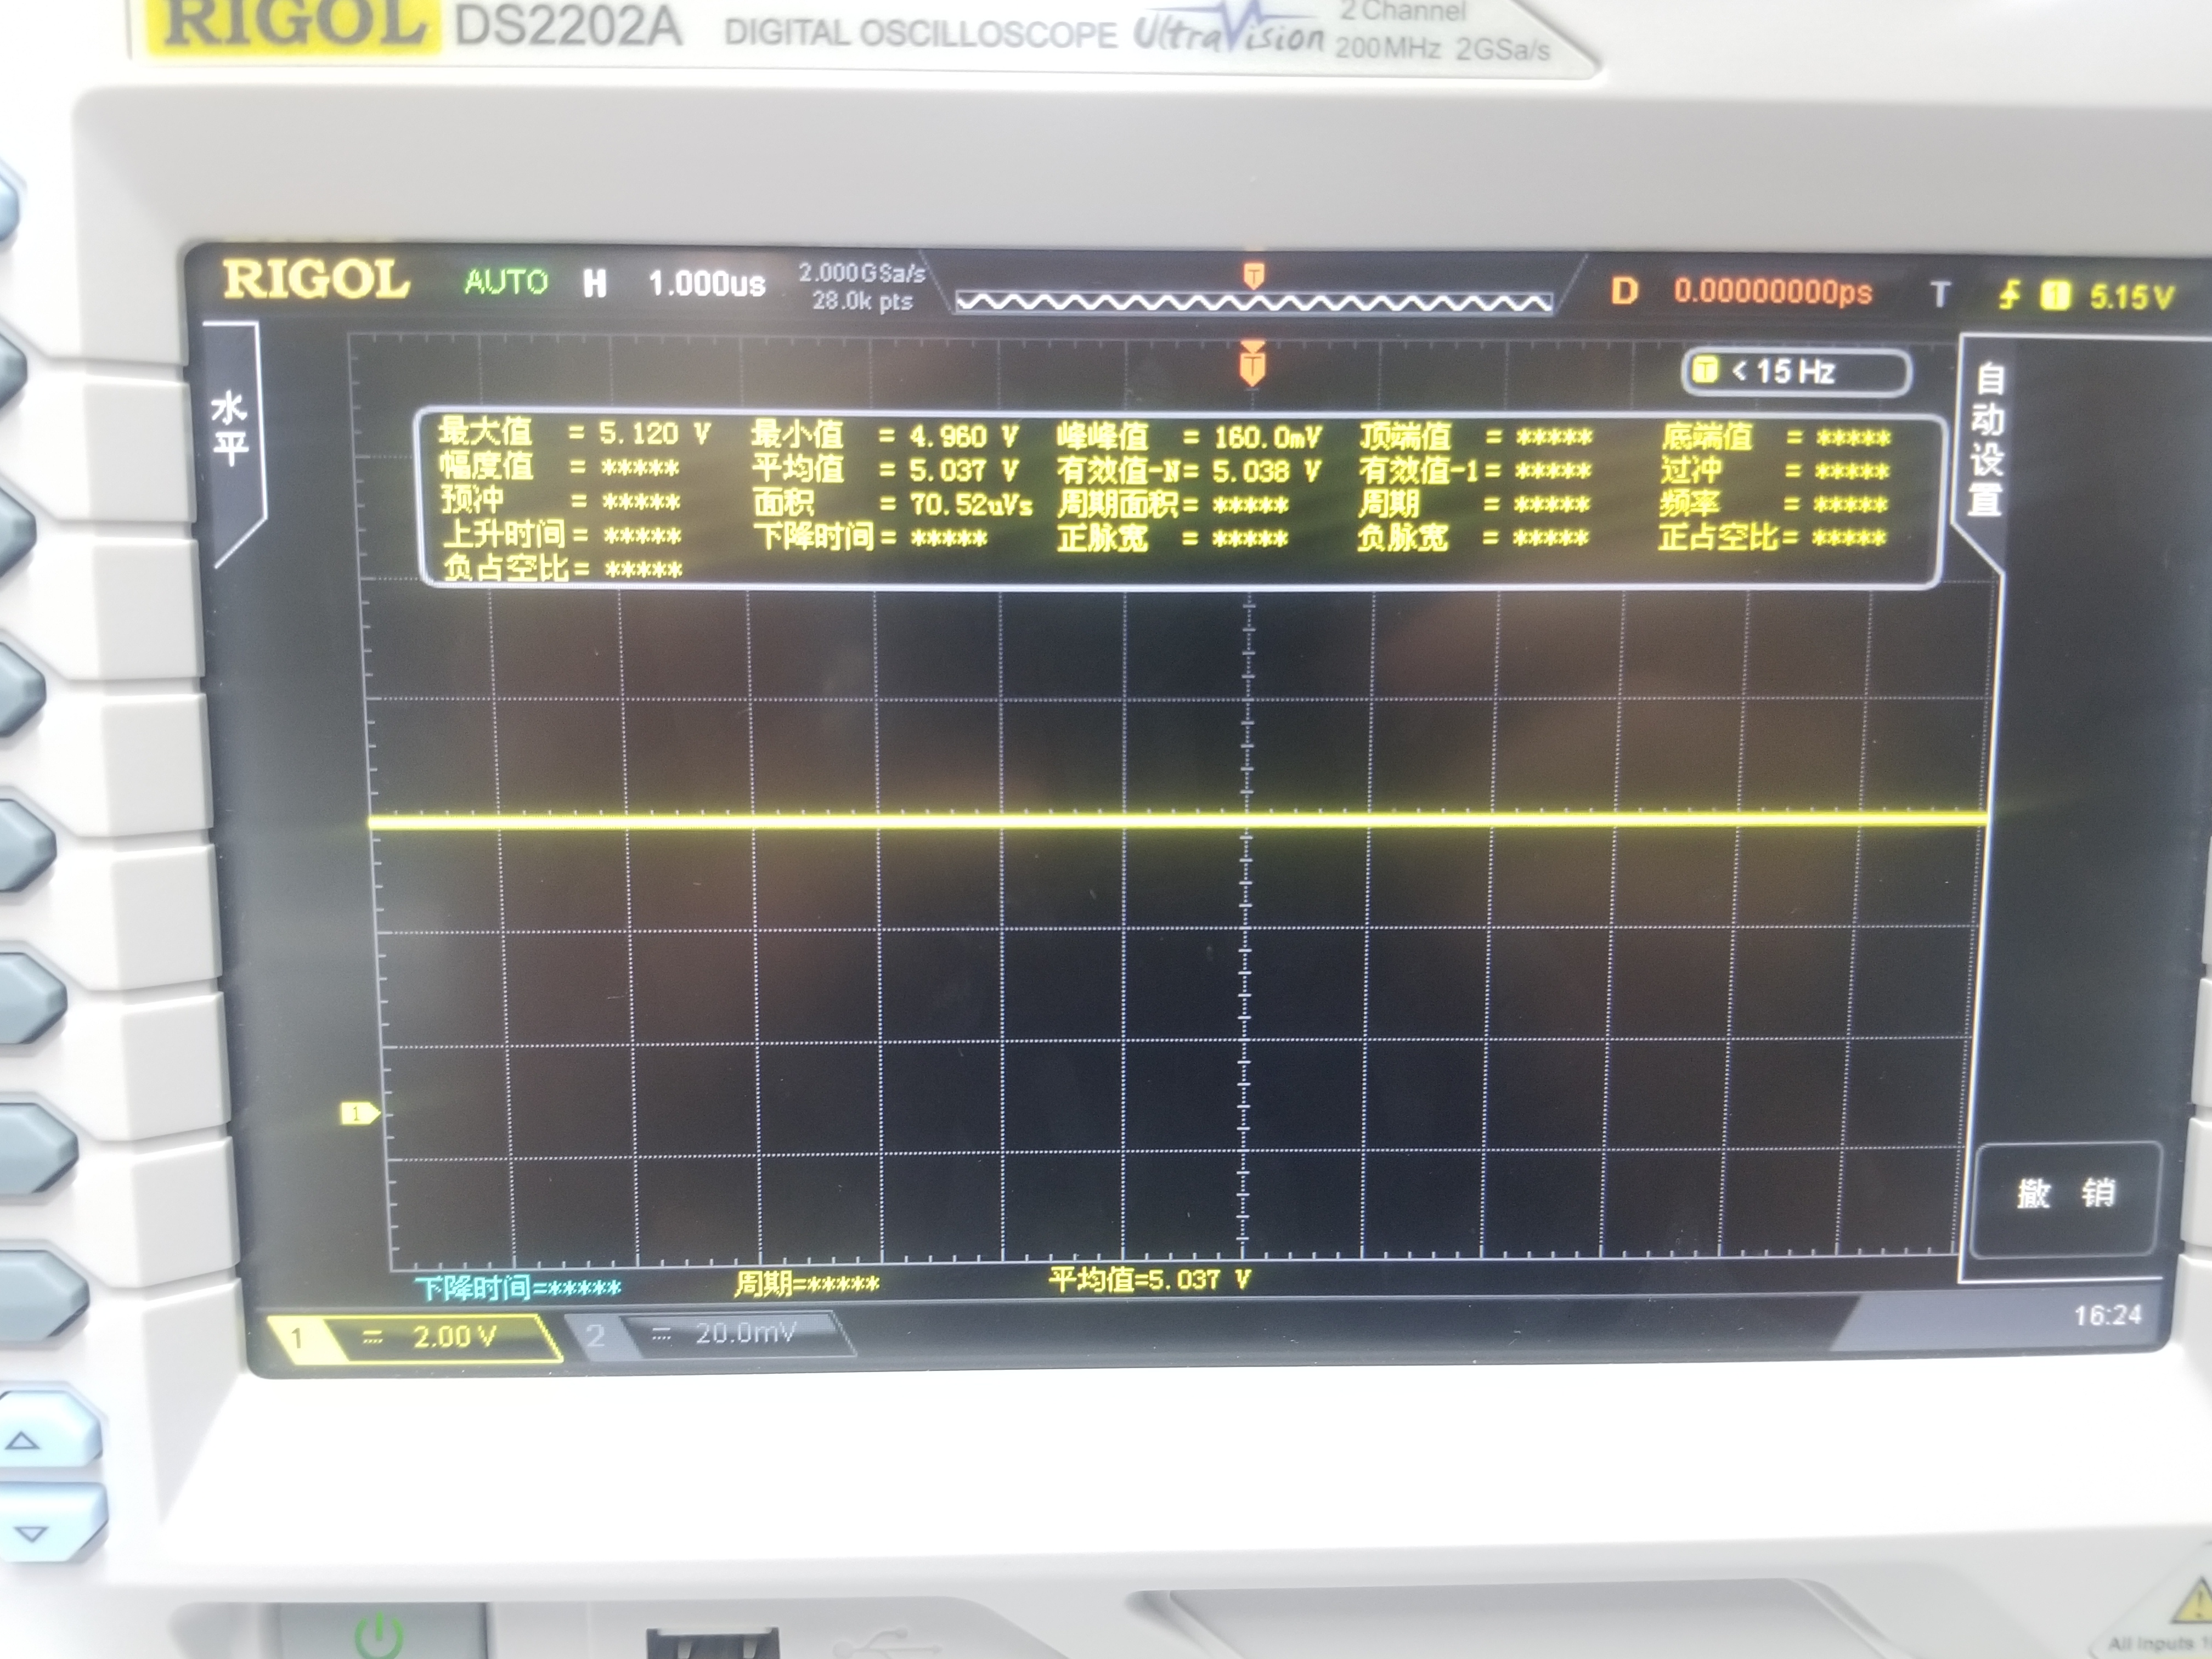
\includegraphics[width=1.5in]{shuju/2/18db_10ms_R}}\\
	\caption{陡降设置分别为$6dB,18dB$,时间常数固定为$10\mathrm{ms}$时示波器上的波形。}
\end{figure}
我们现在对信号做一些改变,观察得到的波形。
\begin{figure}[H]
	\centering
	\subfloat{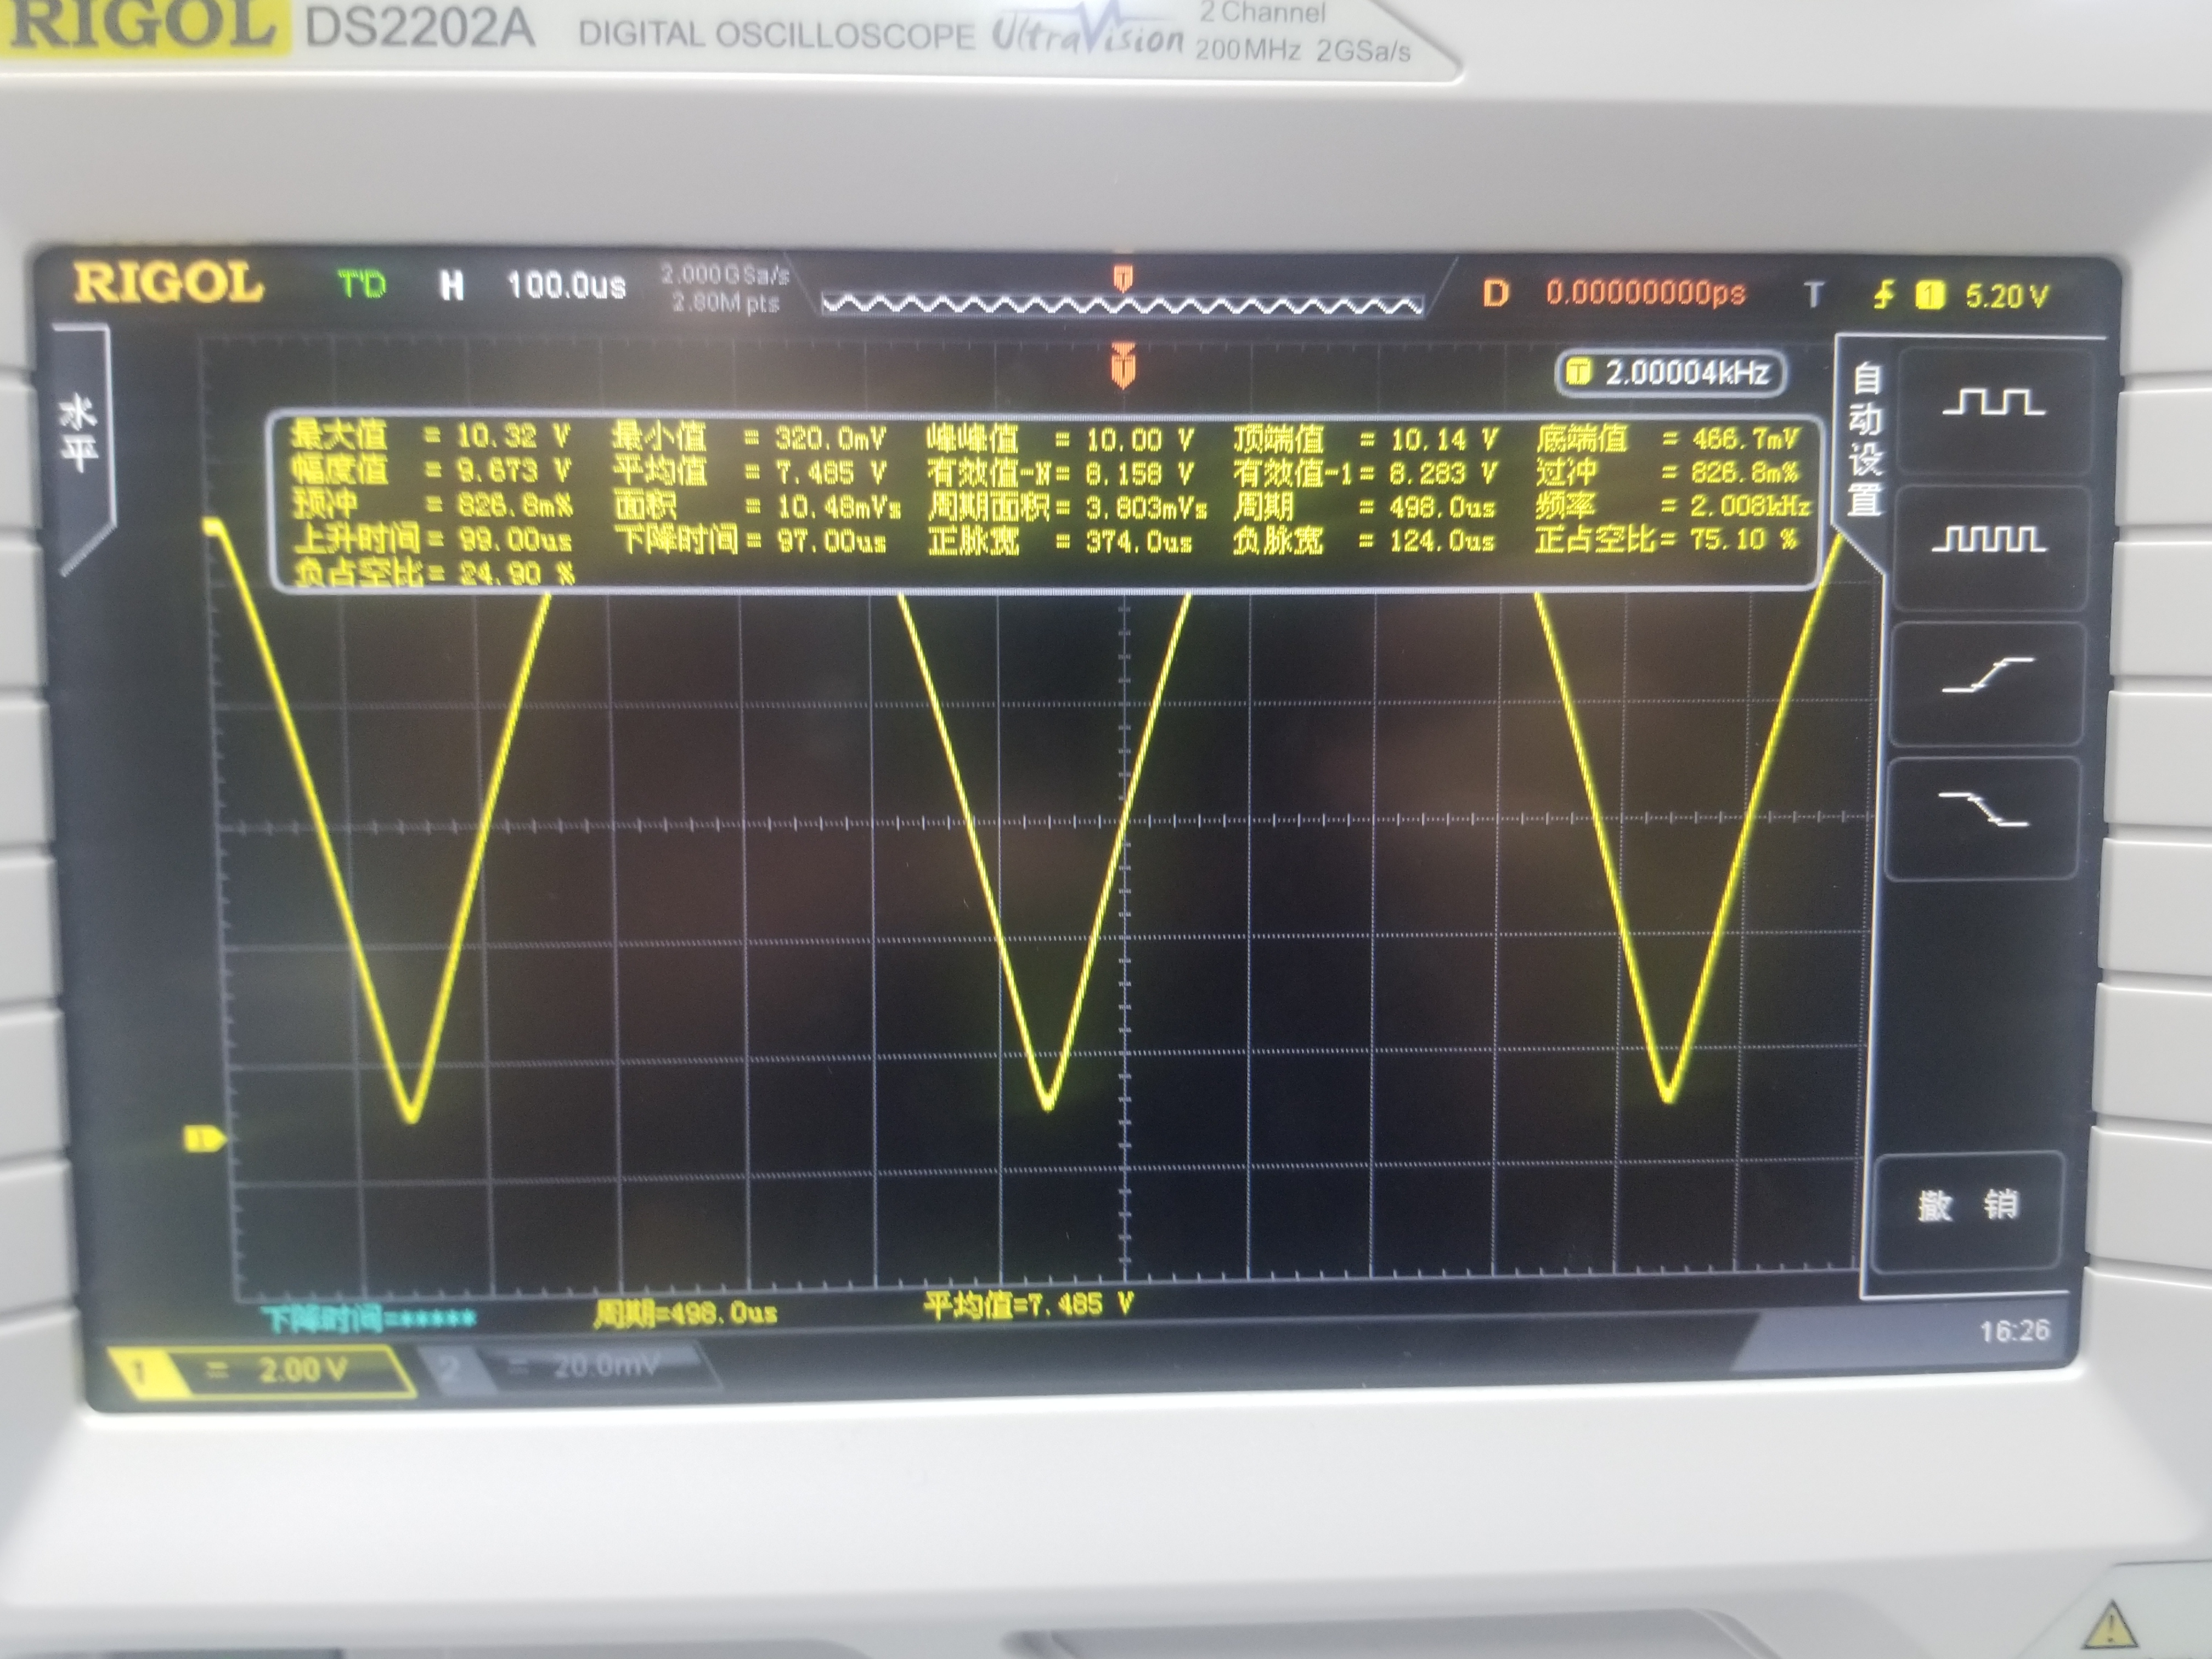
\includegraphics[width=1.5in]{shuju/3/6db_30us_R7}}\quad
	\subfloat{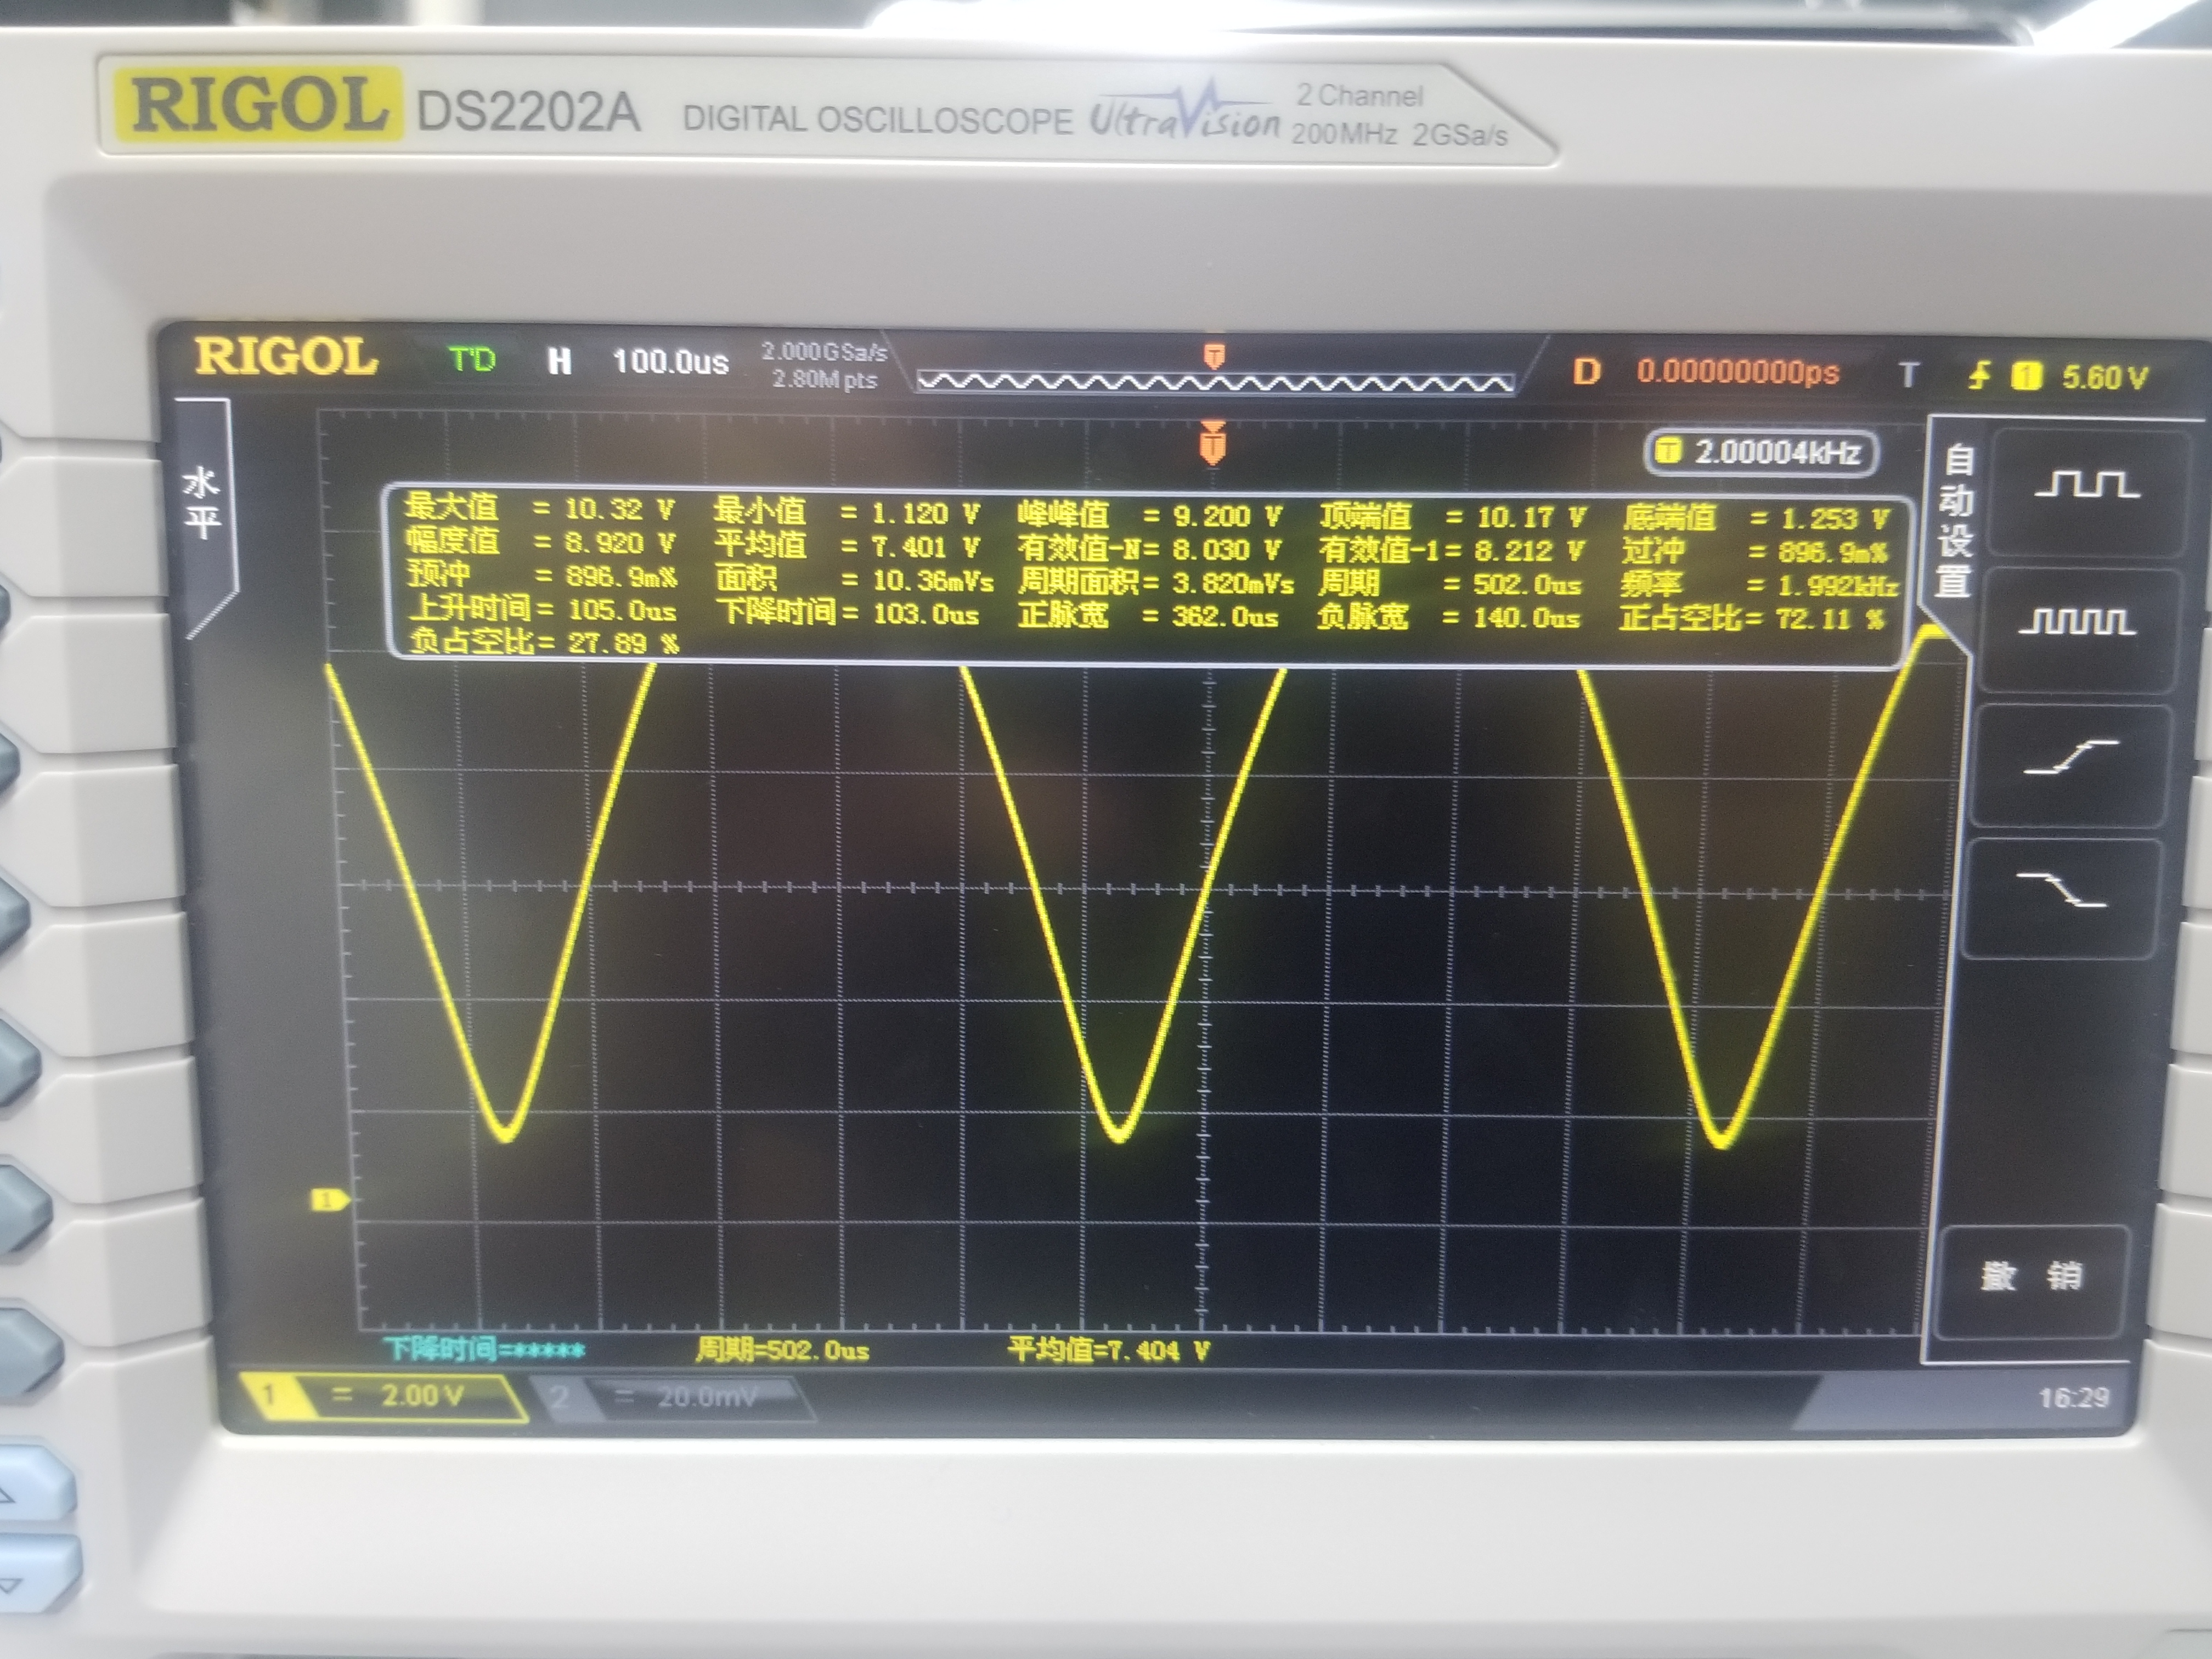
\includegraphics[width=1.5in]{shuju/3/18db_30us_R7}}\\
	\caption{陡降设置分别为$6dB,18dB$,时间常数固定为$30\mathrm{\mu s}$,改变$V_{rms} = 70 \mathrm{mV}$,示波器上的波形。}
\end{figure}
\begin{figure}[H]
	\centering
	\subfloat{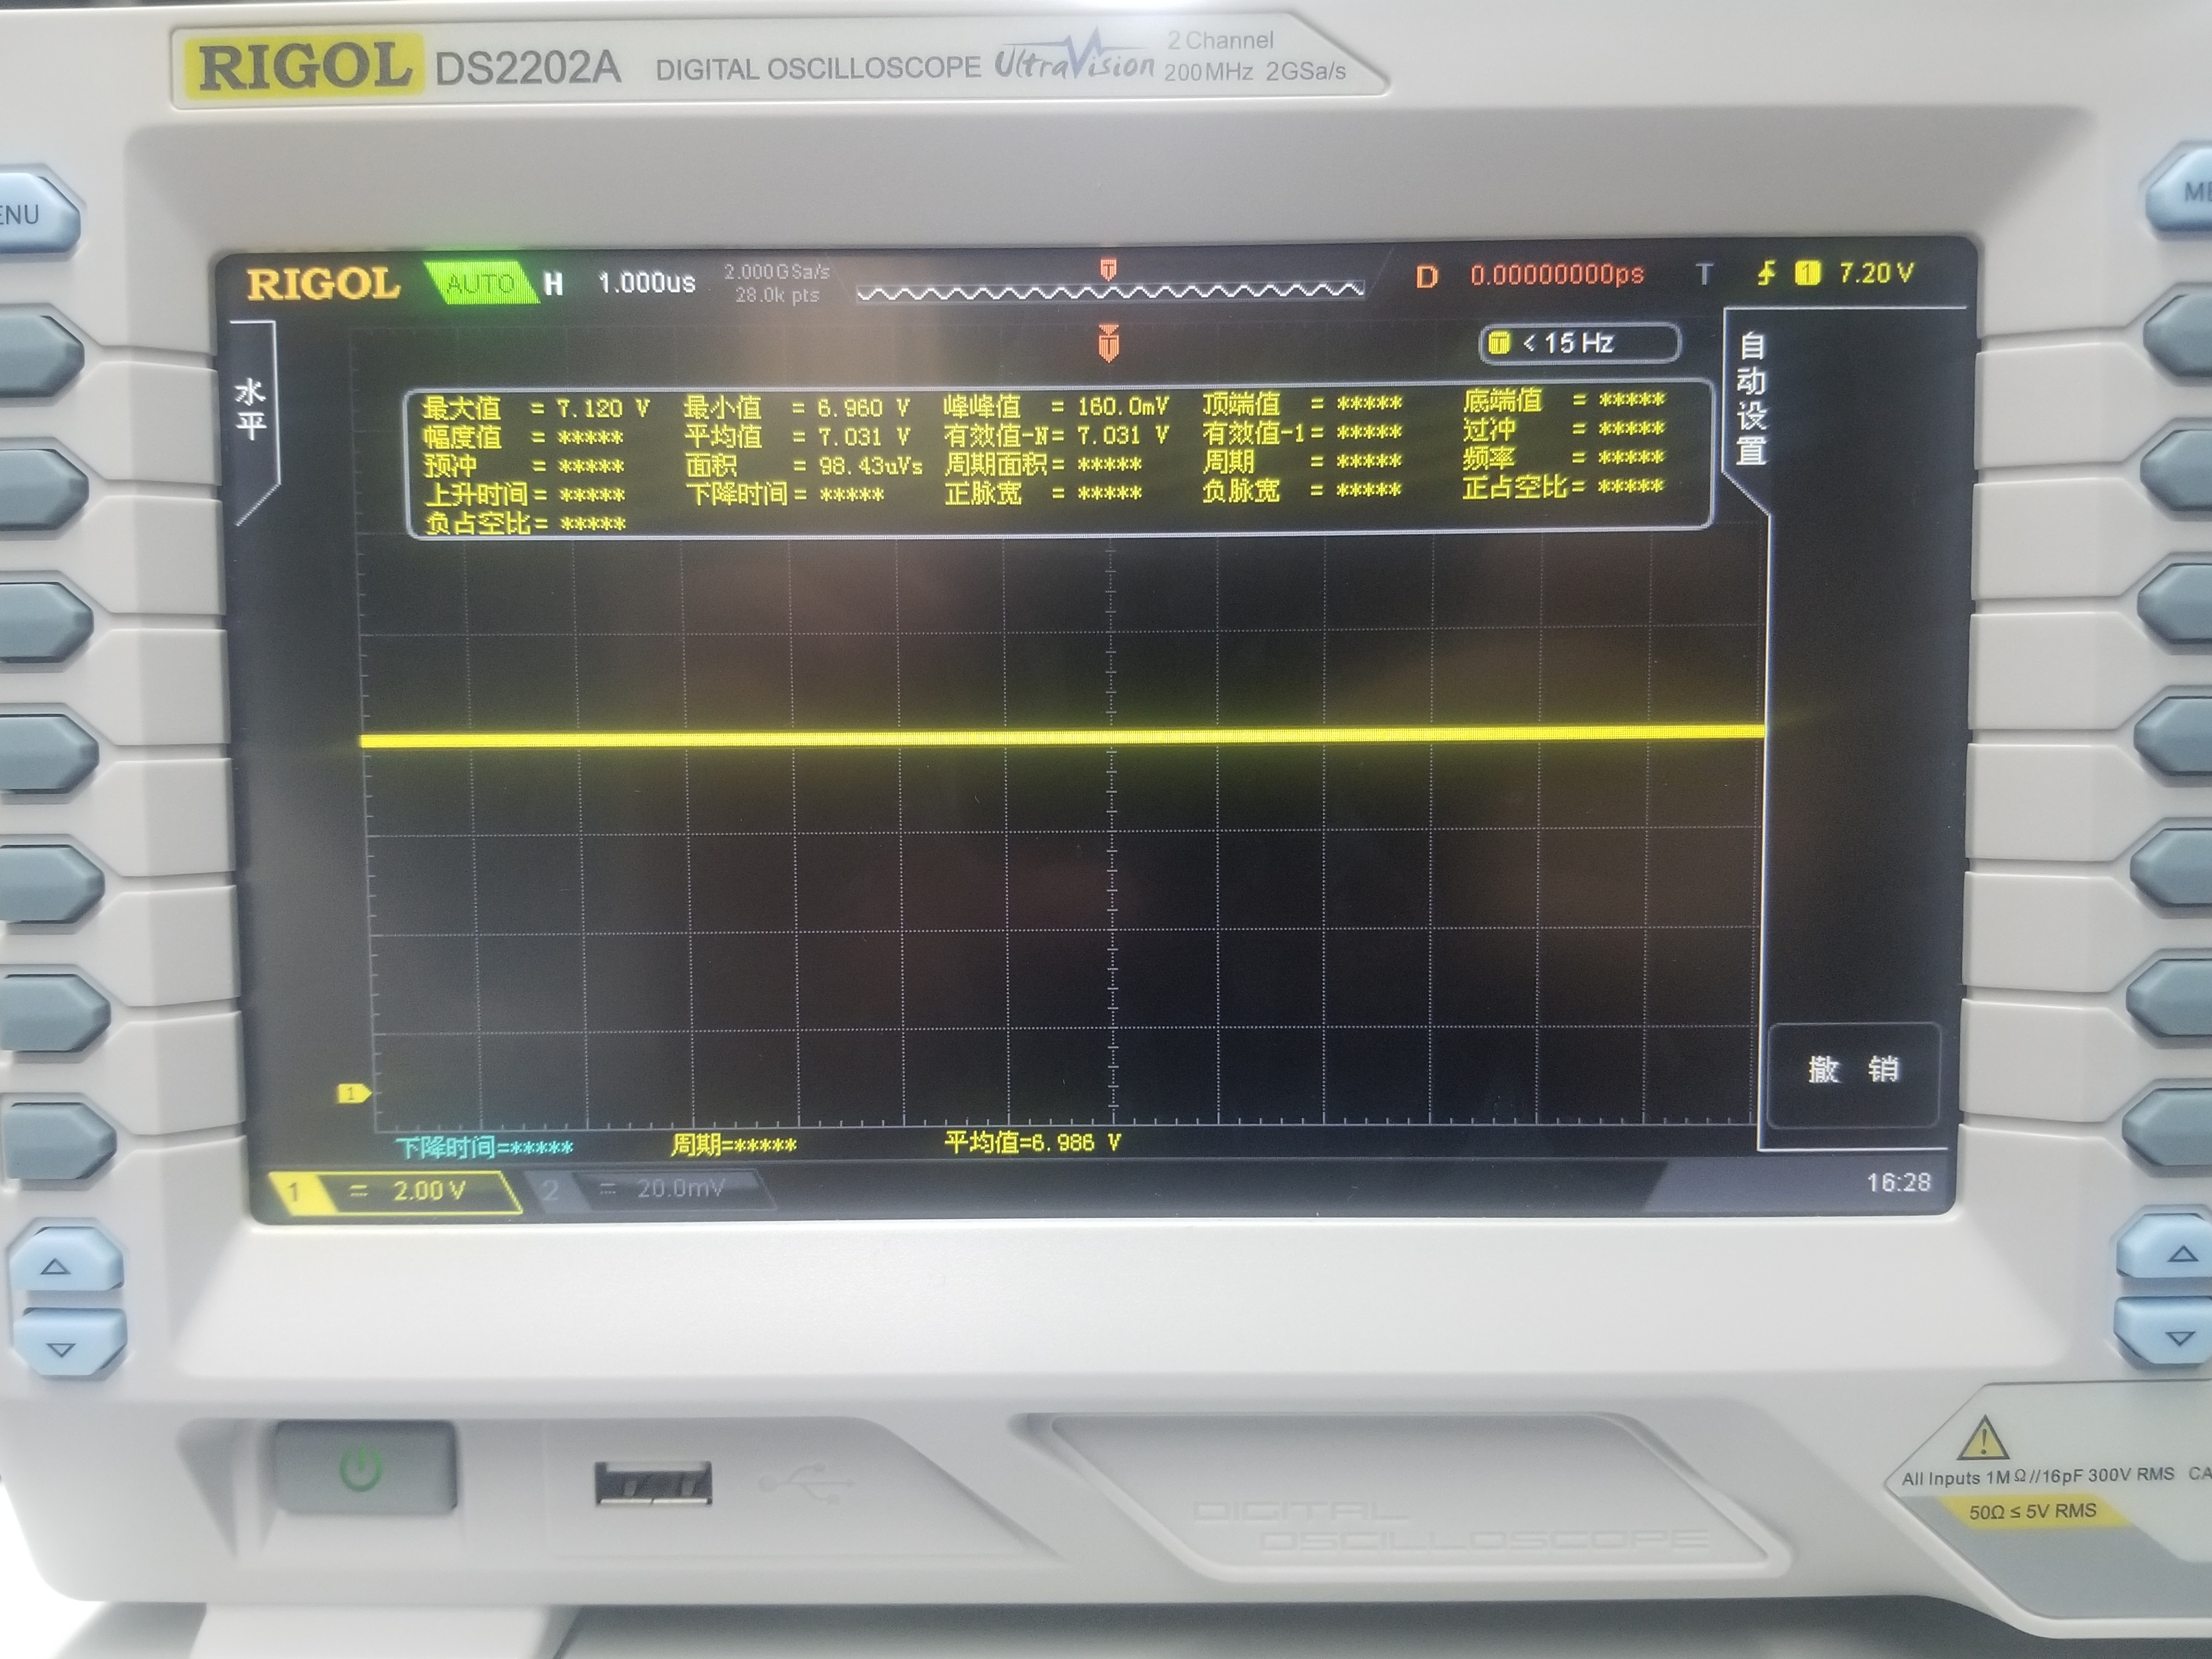
\includegraphics[width=1.5in]{shuju/3/6db_10ms_R7}}\quad
	\subfloat{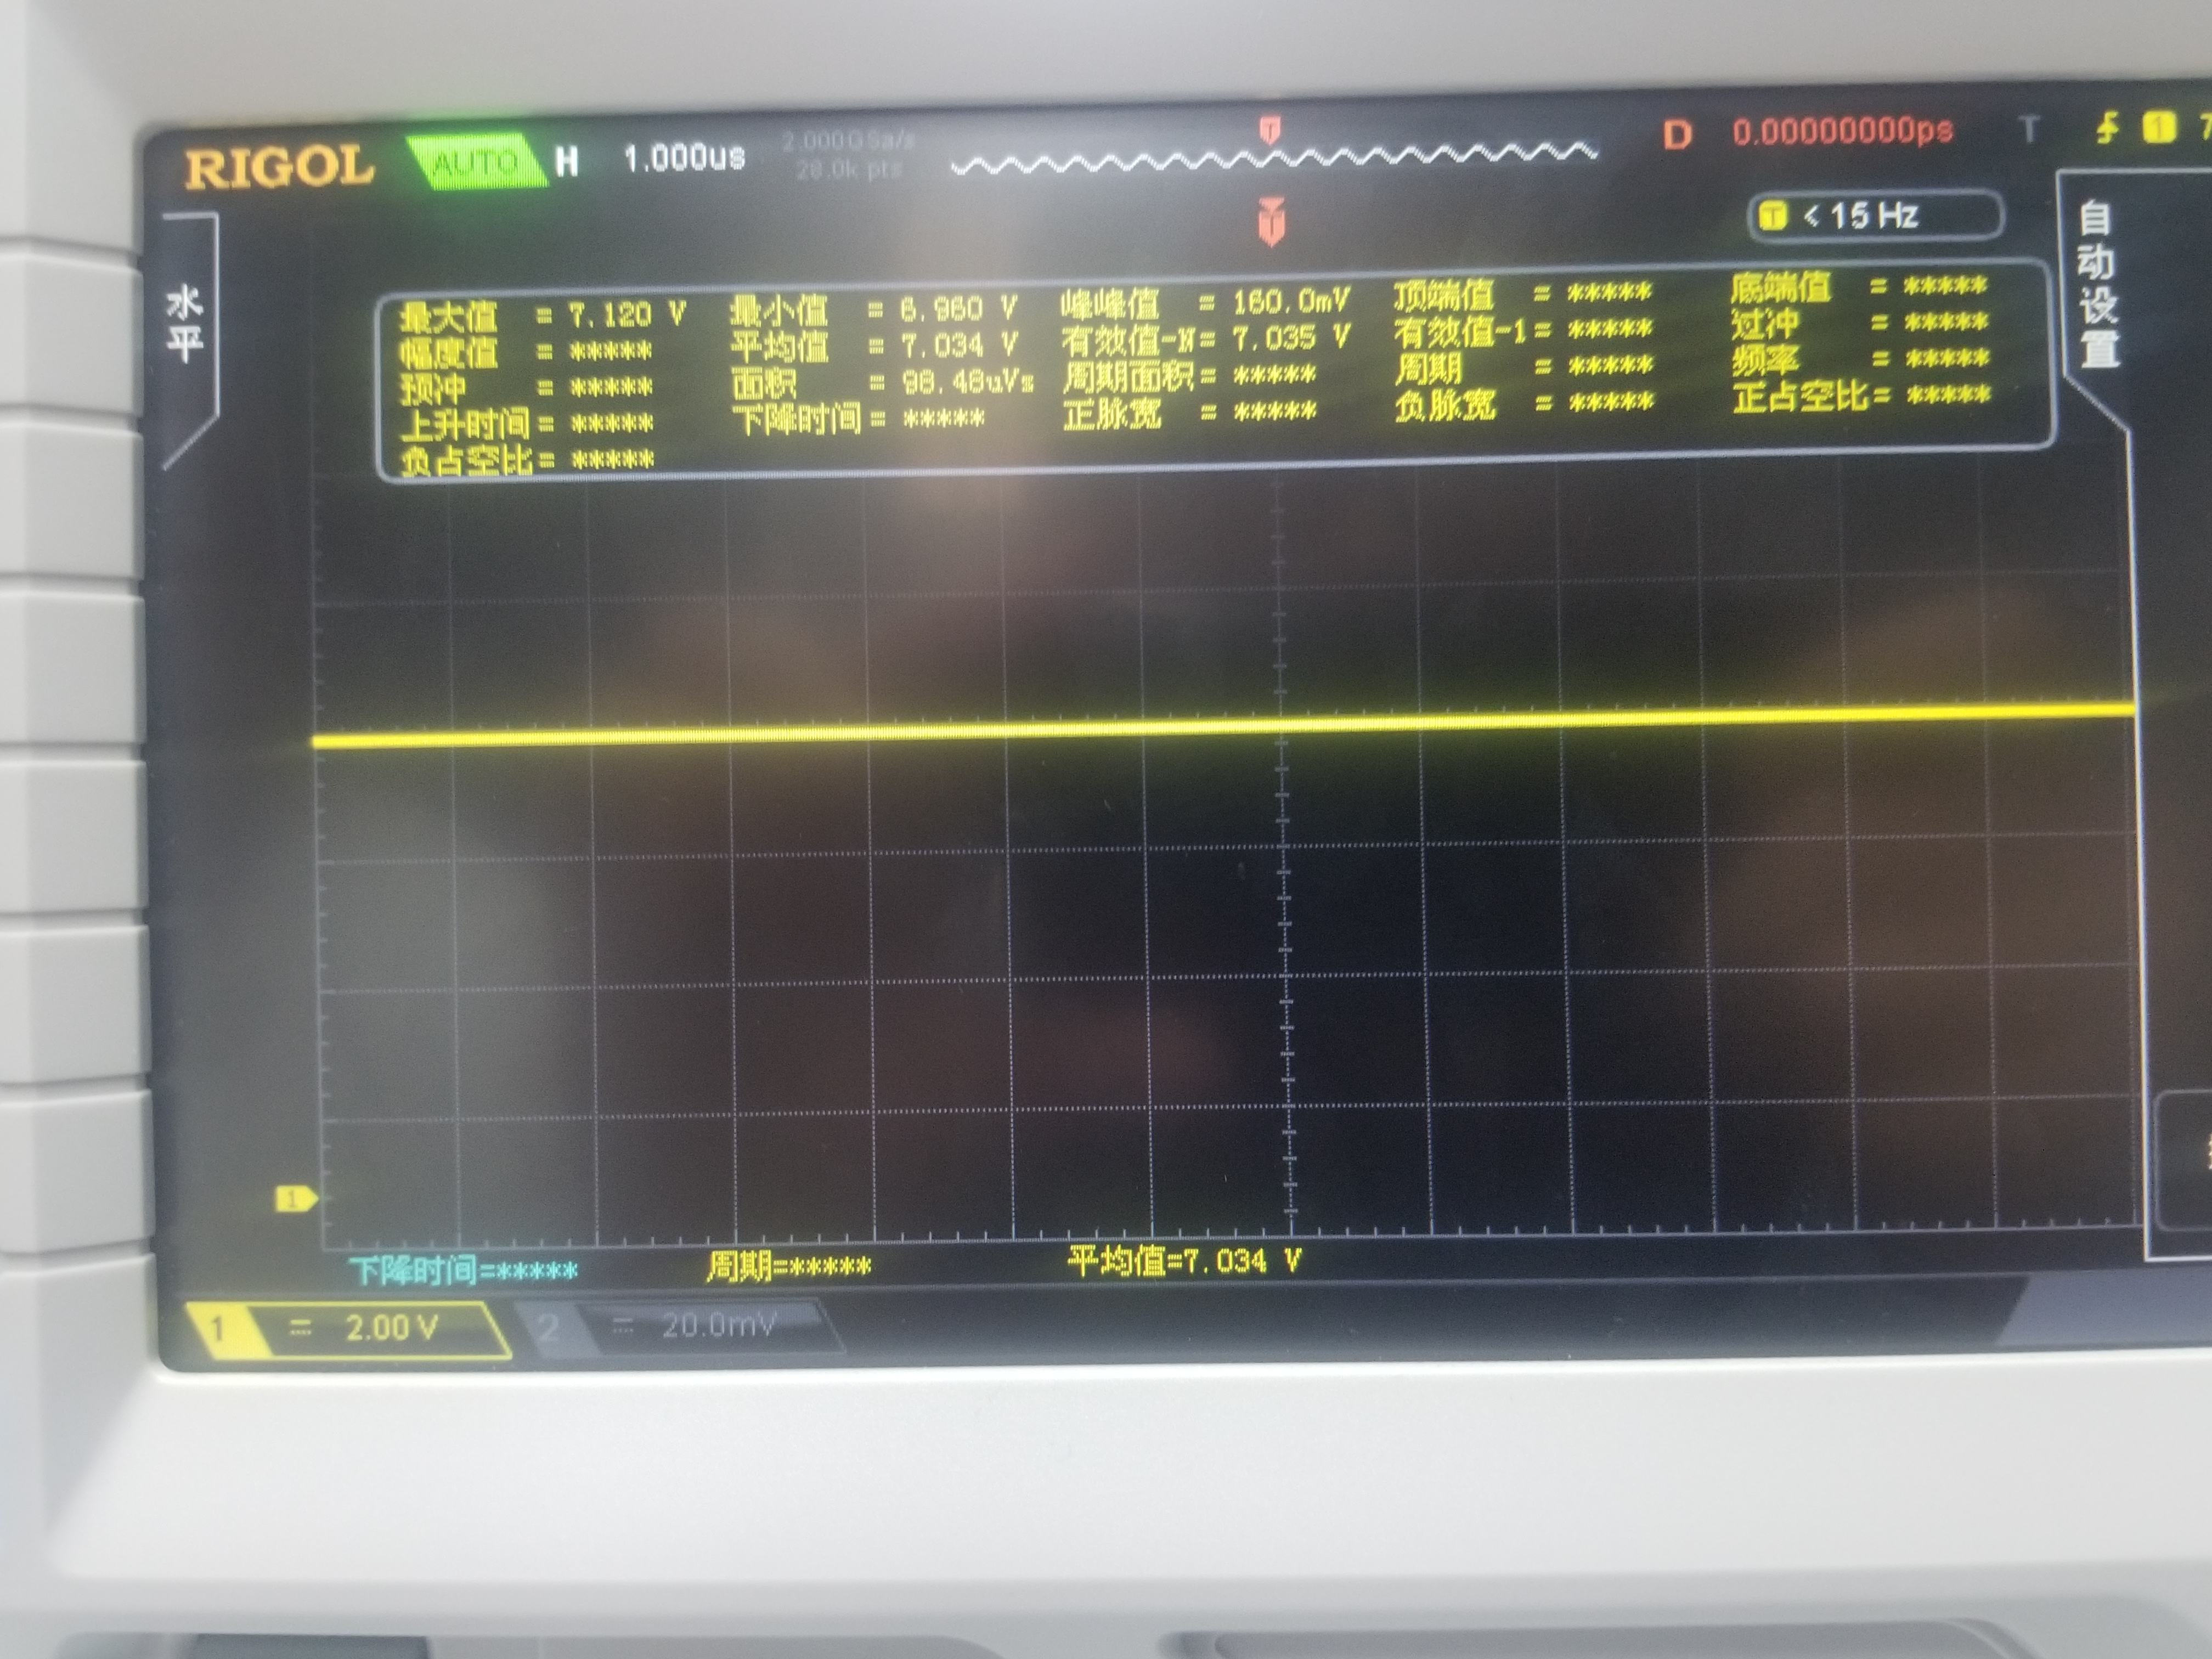
\includegraphics[width=1.5in]{shuju/3/18db_10ms_R7}}\\
	\caption{陡降设置分别为$6dB,18dB$,时间常数固定为$10\mathrm{ms}$时示波器上的波形。}
\end{figure}
\end{enumerate}

由上面的一系列波形,我们可以理解陡降对于锁相放大器的作用:在数字锁相放大器中,低通滤波器是用数字滤波器实现的;同时 OE1022 锁相放大器中可选择 1 至 4 阶低通滤波器级联的结构;不同的阶数对应的滤波器的陡降不同,1 至 4 阶滤波器分别对应 6dB、12dB、18dB、24dB 四种陡降。通过实验数据我们发现,不同的陡降在示波器上的波形的有效值不同。

\subsubsection{探究不同的动态储备对于信号的影响}
\begin{figure}[H]
	\centering
	\subfloat{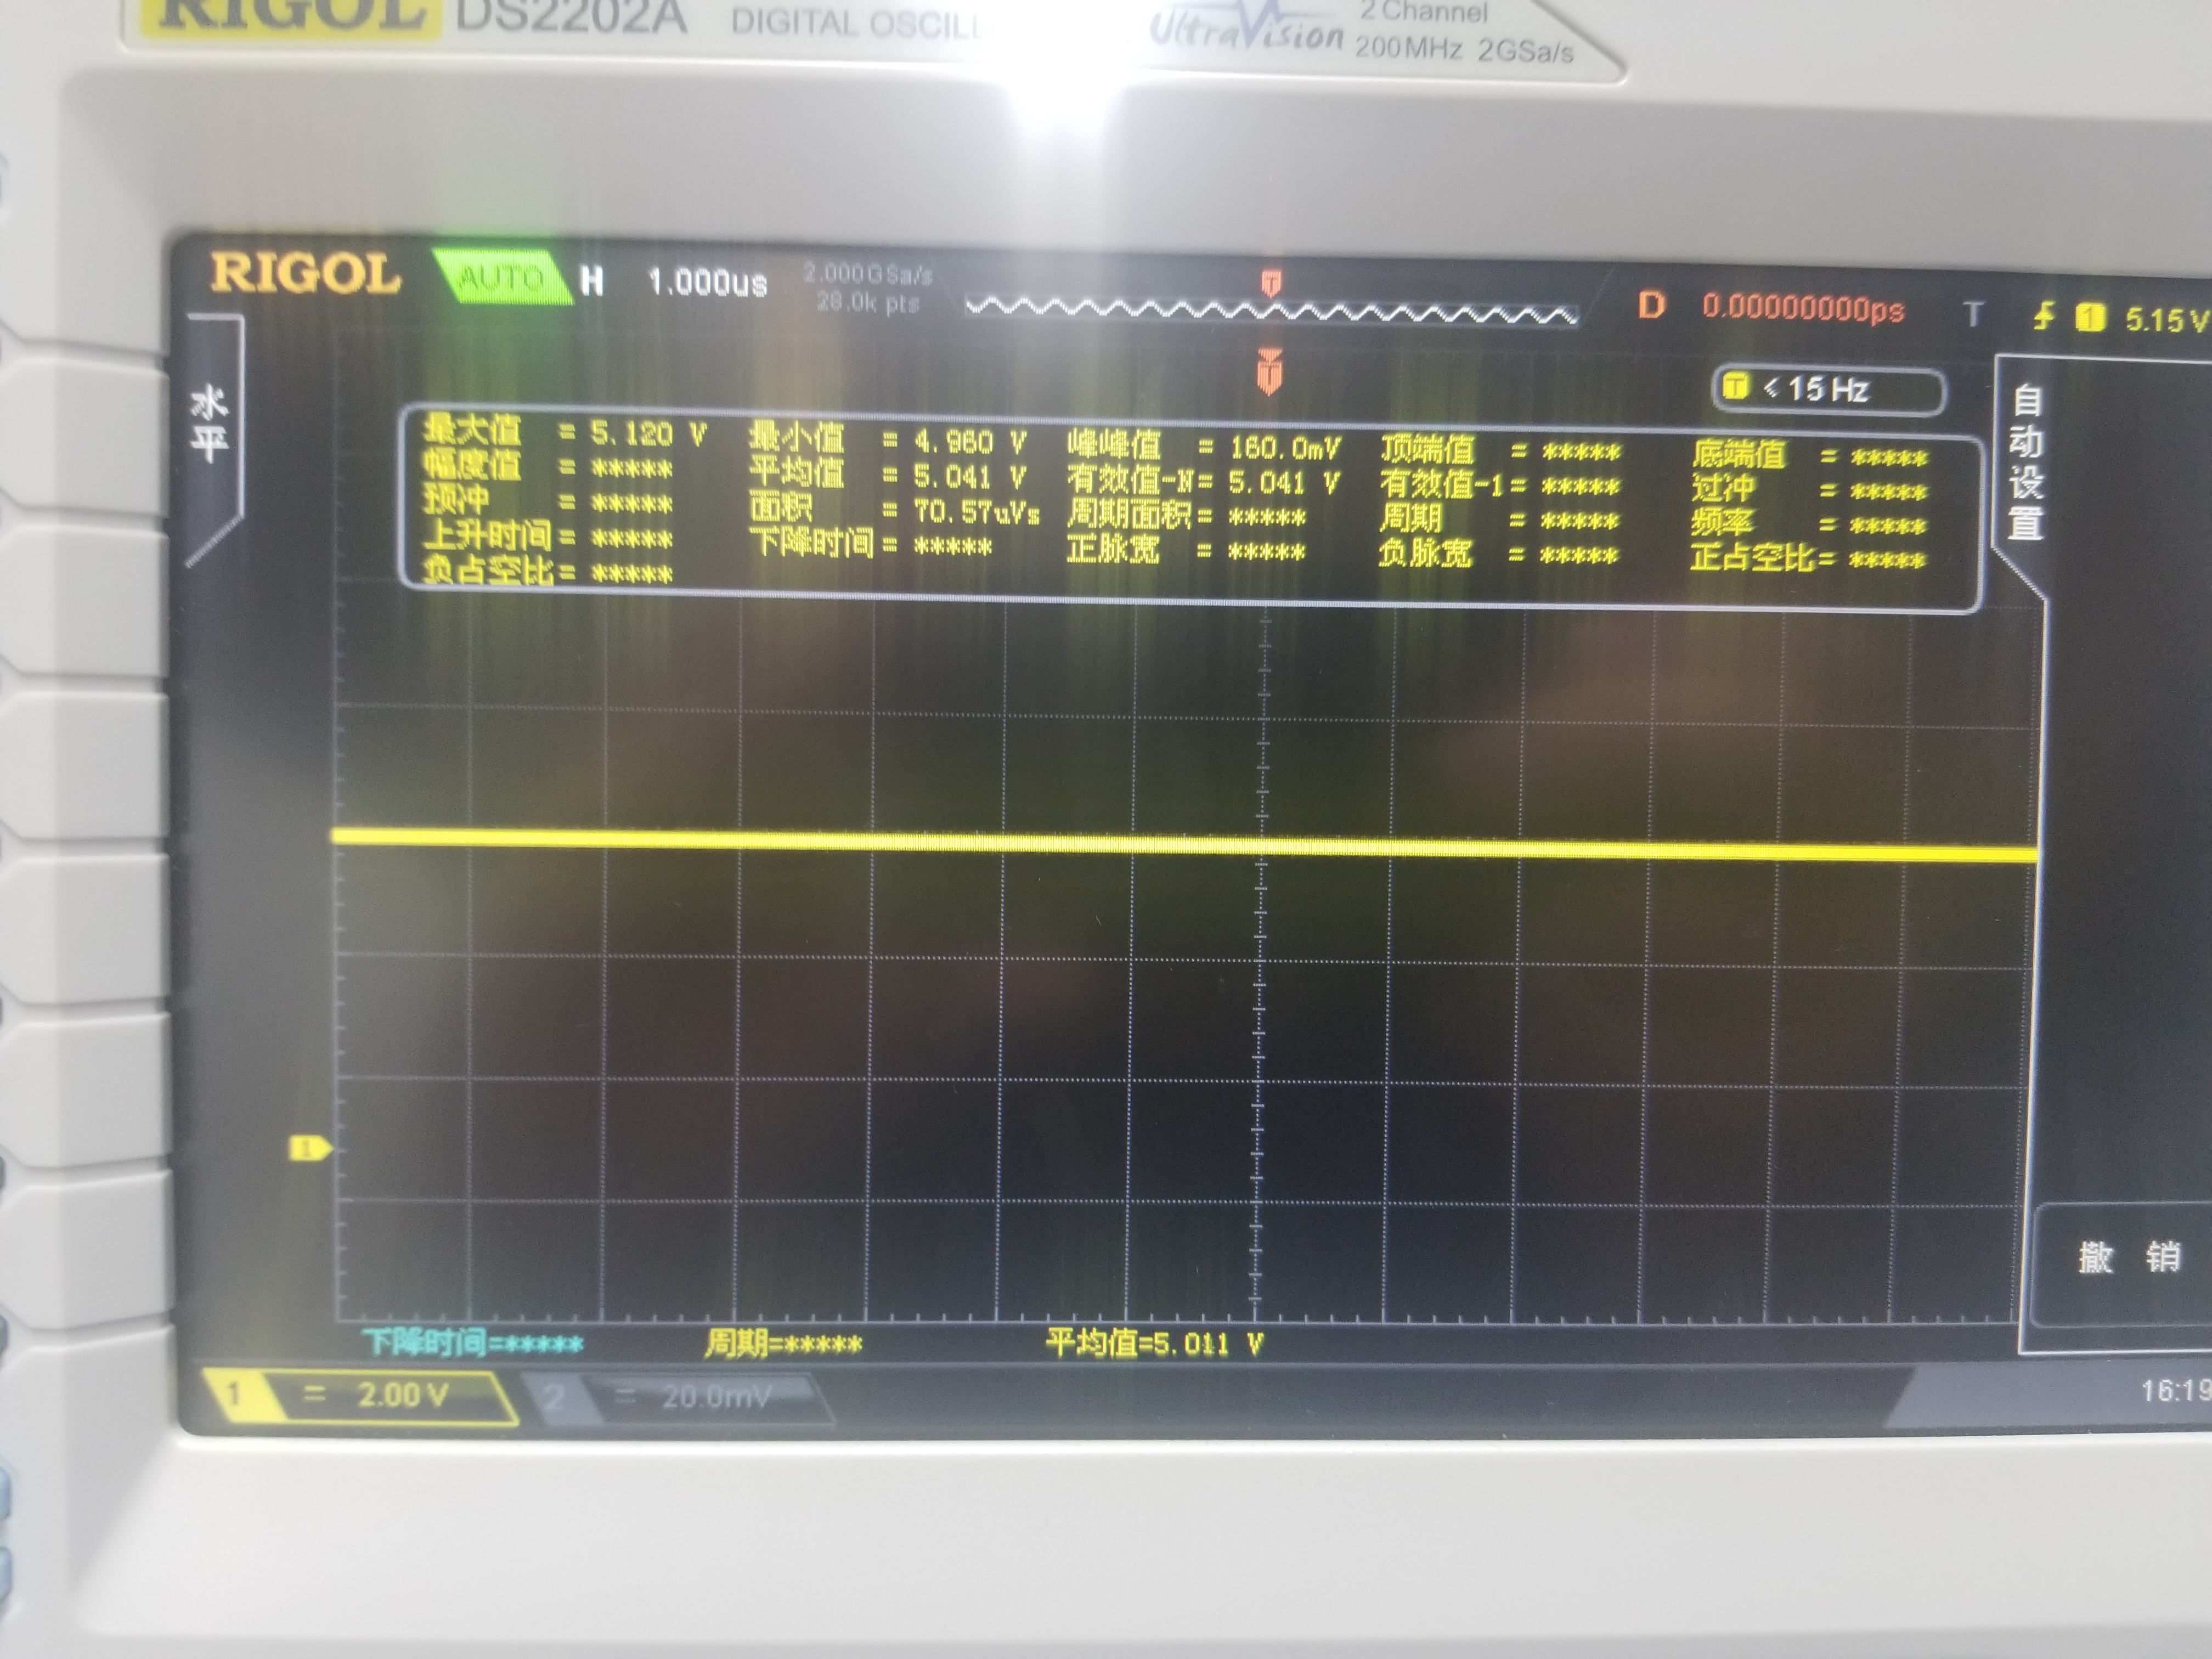
\includegraphics[width=1.5in]{shuju/2/6db_10ms_R}}\quad
	\subfloat{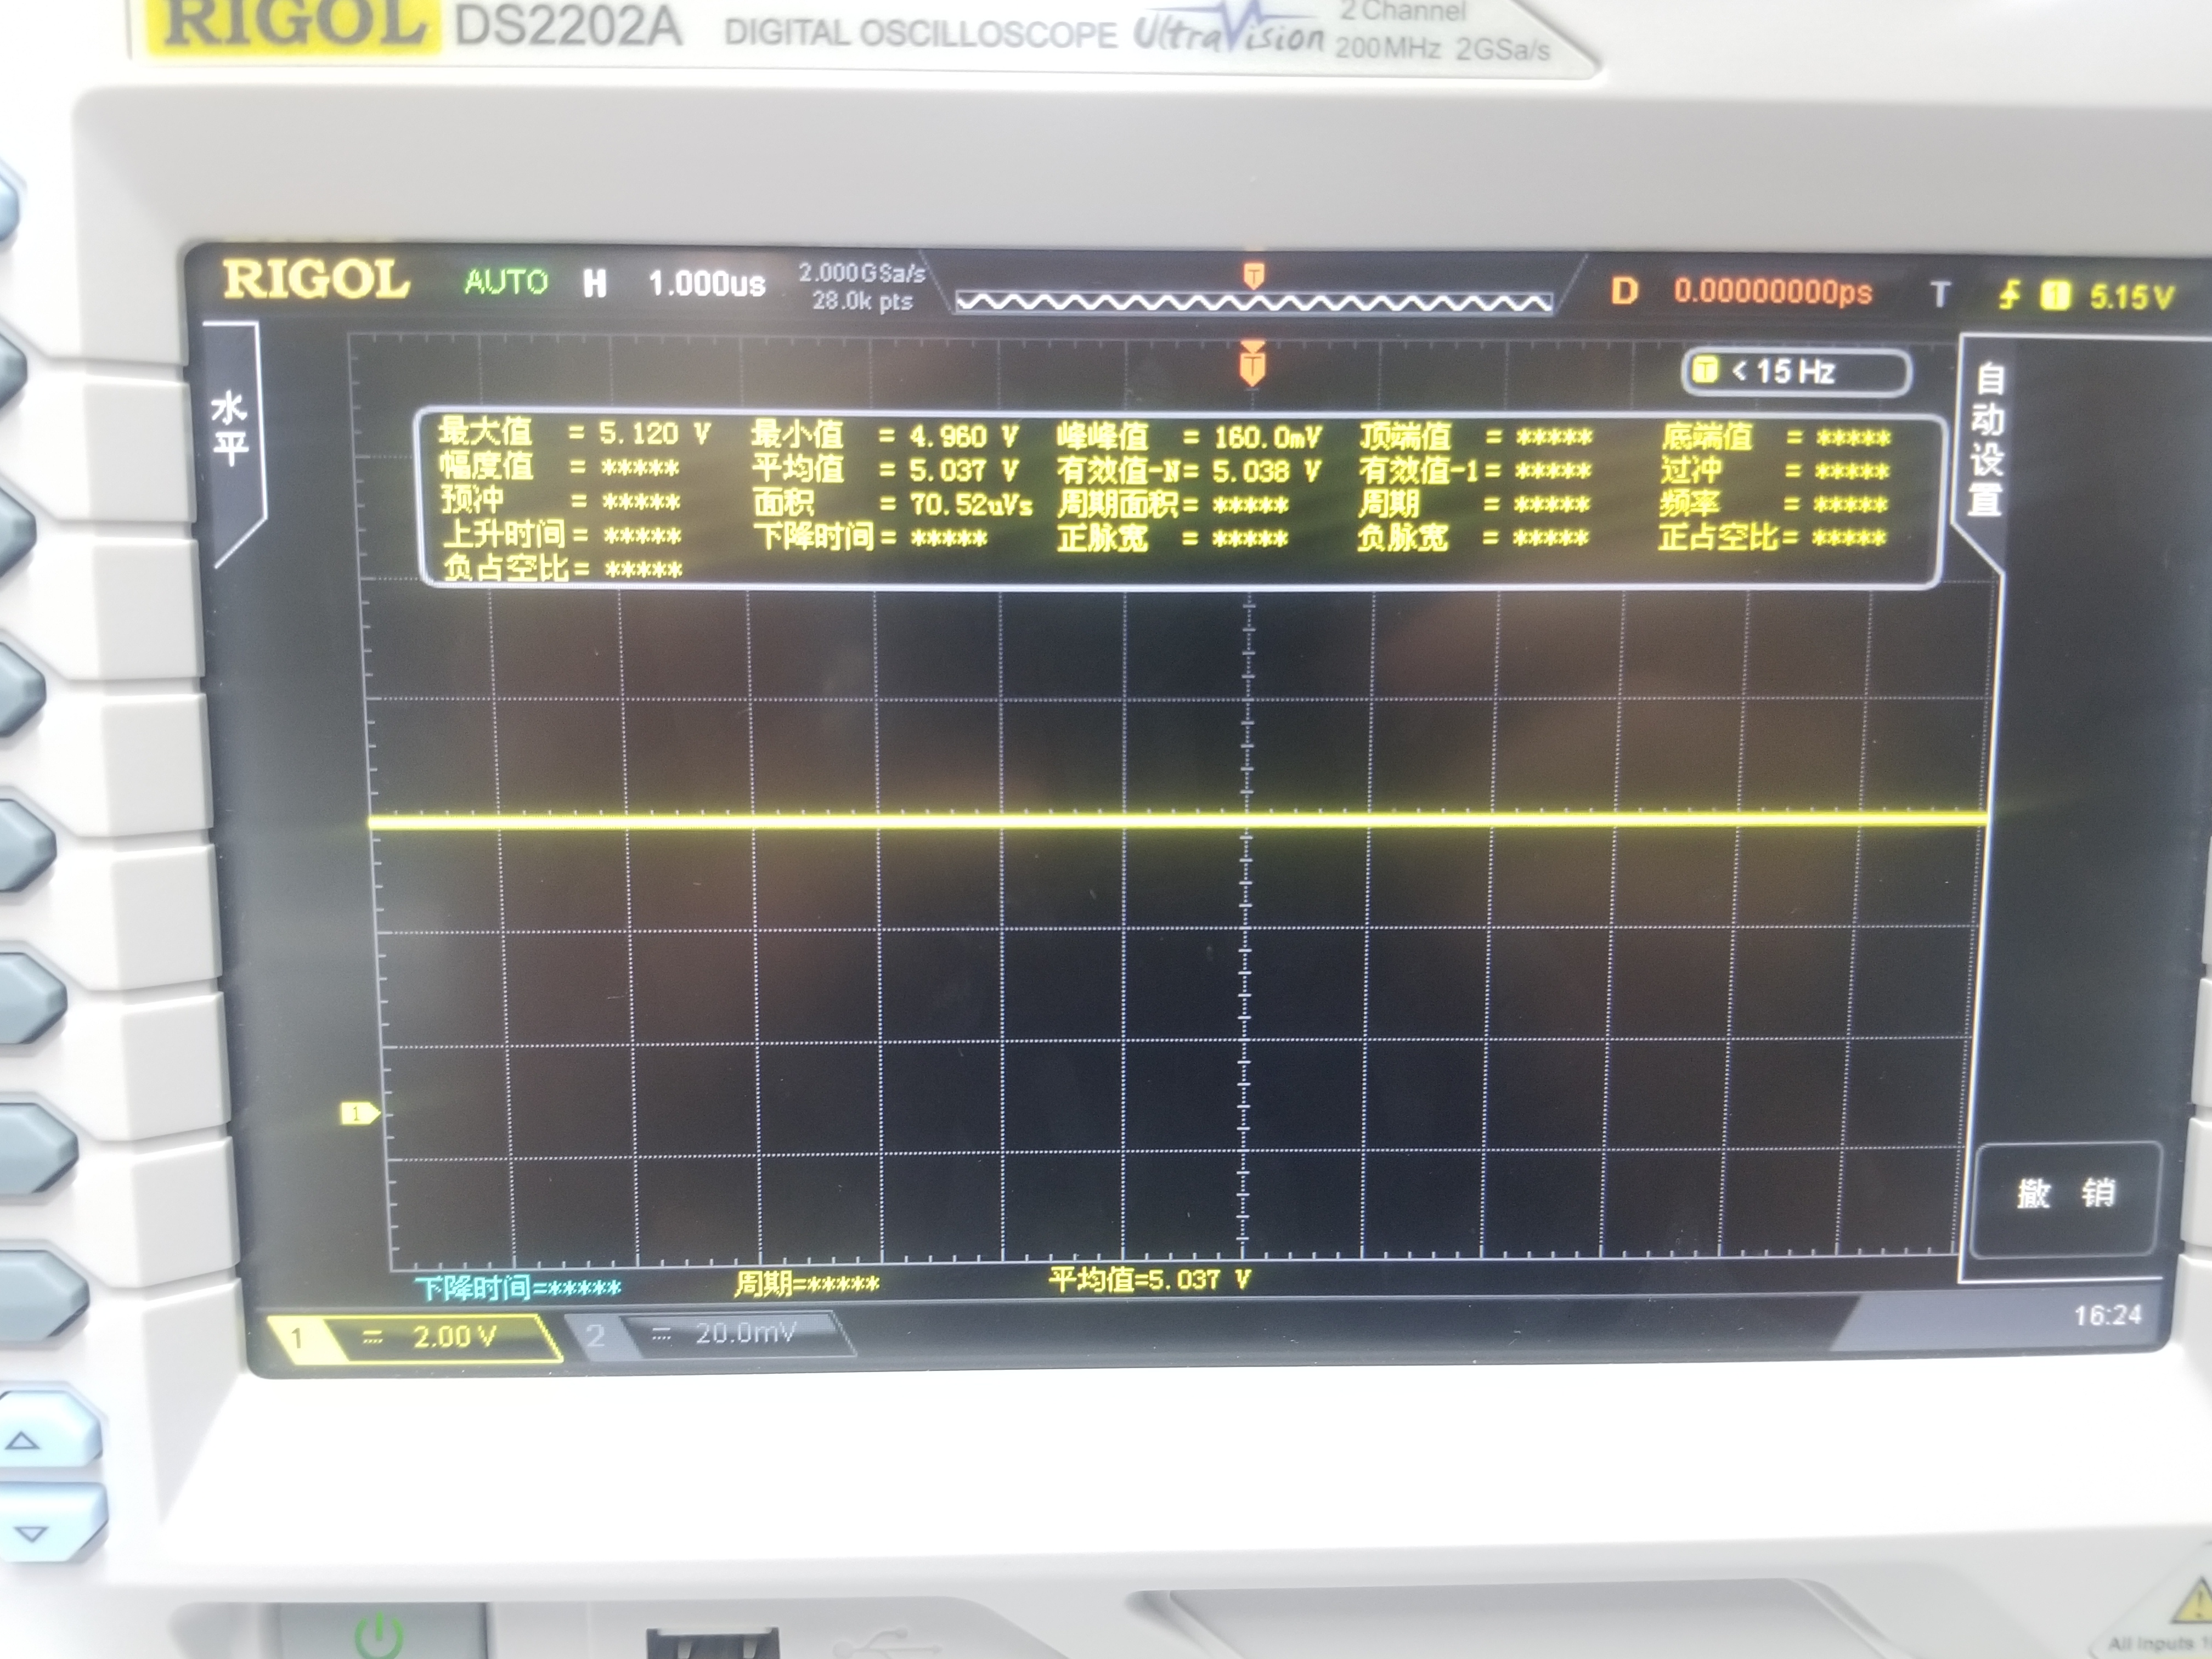
\includegraphics[width=1.5in]{shuju/2/18db_10ms_R}}\\
	\caption{陡降设置分别为$6dB,18dB$,时间常数固定为$10\mathrm{ms}$时示波器上的波形。}
\end{figure}

\subsubsection{外部输入参考信号}
在实验中,我们使用BNC-BNC信号线连接了{\color{red} 信号发生器}输出接口和SIGNAL IN 的A/I接口,通过改变参考信号相位,我们获得的$R,\theta,X,Y$数据见上节附录。通过数据软件使用最小二乘法~\cite{error}使用正弦曲线对数据$\theta,X$进行拟合,如~\cref{theta&x_2}所示。
\cpicn{0.5}{theta&x_2}{$\theta$和$X$的拟合曲线}
在拟合过程中,我们使用拟合系数$R^2$来表征拟合的好坏,设待拟合数据为$y$,拟合出来的对应曲线上的点为$f$,则拟合系数定义为
\beq
R^2 = 1-\frac{\sum_i(y_i - f_i)^2}{\sum_i (y_i-\bar{y})^2}
\eeq
由上述公式我们计算得到,拟合曲线的拟合系数为
\beq
R^2 = 0.99999
\eeq
通过数据软件使用最小二乘法使用正弦曲线对数据$\theta,Y$进行拟合,如~\cref{theta&y_2}所示。
\cpicn{0.5}{theta&y_2}{$\theta$和$Y$的拟合曲线}
在拟合过程中,我们使用拟合系数$R^2$来表征拟合的好坏,设待拟合数据为$y$,拟合出来的对应曲线上的点为$f$,则拟合系数定义为
\beq
R^2 = 1-\frac{\sum_i(y_i - f_i)^2}{\sum_i (y_i-\bar{y})^2}
\eeq
由上述公式我们计算得到,拟合曲线的拟合系数为
\beq
R^2 = 0.99999
\eeq
可见,$X,Y$确实随着$\theta$的变化满足正弦和余弦的关系。

对于外部输入参考信号的情况,我们也改变频率来测量频率对于相位差的影响,对于外部输入的参考信号,改变频率,我们没有发现相位角有任何变化(数据见上节附录),这正如我们的理论所预言。因为这一相位差随着频率的变化是由于电磁波信号在电缆中传播而产生的,如果是外接信号,则参考信号和调制信号都是输入进来的信号,没有任何差别,所以调制后的信号和调制信号,当频率改变时,他们的相位差不会有任何显著的变化。

\subsubsection{示波器观察噪声发生器的输出噪声是否为白噪声}
\cpicn{0.2}{white_noise}{噪声发生器产生的噪声接入示波器,示波器上面显示的是时域图,下面显示的是频域图}
在实验中,我们将实验箱中噪声发生器产生的噪声接入示波器,得到时域和频域的图像如上图所示,在时域图中,我们发现噪声完全是混乱的,没有任何规律或者严格的周期性可言,这意味着在频域上它也是几乎处处均匀的,以至于不同频率的振动取平均之后均抵消。在实验中,我们选示波器上的傅里叶变换功能,观察到在频域上的信号确实如我们预言。
\subsubsection{比较OE1022示波器对于不同信号强度和信噪比的测量结果}
实验中改变不同信噪比测得的数据如下表所示(第二部分有原始记录)
\begin{table}[H]
\centering
\begin{tabular}{ | p{2cm} | p{2cm} | p{2cm} | p{2cm} | p{2cm} |}
\hline
 正弦波$V_in$幅值(m$V_{rms}$) & 噪声信号大小(m$V_{rms}$) & 信噪比(dB)&锁相放大器测量R(m$V_{rms}$) & 示波器测量值(m$V_{rms}$)\\
\hline
	1000  & 100 &20 &1006.5 &1037  \\
\hline
	100	  & 100 & 0 &100.47 &104.8 \\
\hline
	10 &100  & -20 &10.05 &11.83 \\
\hline
	1 & 100 &-40  &1.01 &1.02 \\
\hline
\end{tabular}
\end{table}
由上面的对比可以看到,当信噪比很小时,锁相放大器的测量与示波器的测量差别不大,当信噪比大时,锁相放大器测量的结果明显更加接近真值。但是即使是信噪比很小的情况,锁相放大器仍然比示波器精确。
\subsection{实验后思考题}
\subsubsection{实验一}

1. OE1022 的正弦输出(SINE OUT)与通道输出(CH OUT)分别输出什么信号?

SINE OUT输出:是由OE1022自带的信号发生器输出的信号,当外部参考信号使用时,信号发生器通过锁相环与输入信号进行锁相。

CH OUT输出:根据当前测量信号的测量结果与当前设置测量范围的比例,正比到输出。

2. Ref.phase 会改变 SINE OUT 输出信号的相位角吗?

不会改变SINE OUT输出信号的相位角,改变的是参考信号的相位角。将输出信号SINE OUT接到示波器上,改变Ref.phase的值,发现示波器上的波形图没有任何变化。

3. 为什么改变参考信号的频率对相位差$\theta$的测量值有影响?如果我们要考查相位差对其他变量的响应时,对不同的频率相位差是否都要重新置零?

这里的相位差$\theta$实际上是调制后的信号相对于解调信号的相位差。在理论上,随着频率的改变,这一相位差应该不变。但是在实际中,参考信号是通过某种物理机制触发的,在实验中,我们观测到,随着频率的不断升高,$\theta$值变化的很小,但是近似为线性减少。因此,由于电缆的存在,信号在电缆中传播会引起额外的相位差,这一部分的相位差贡献到了调制后的信号的相位中,因此产生了相位差。根据介质中的麦克斯韦方程组(例如,参见~\cite{electromagnetic})
\bea
\nabla \cdot \vec{E} &=& \rho/\epsilon \\
\nabla \times \vec{E} &=& -\frac{\partial \vec{B}}{\partial t} \\
\nabla \cdot \vec{B} &=& 0\\
\nabla \times \vec{B} &=& \mu\vec{j} + \mu\epsilon \frac{\partial E}{\partial t}
\eea
利用公式
\beq
\nabla\times( \nabla\times \vec{E} ) =  \nabla(\nabla \cdot \vec{E}) - \nabla^2 \vec{E}
\eeq
将麦克斯韦方程组带入上式两边,利用欧姆定律,并取$\rho = 0 $,得到
\beq
\frac{\partial^2 \vec{E} }{\partial t^2}+\mu \sigma \partial_t \vec{E} - \frac{1}{\mu\epsilon} \nabla^2 \vec{E} =0
\eeq
上式实际上是一个波动方程,$\mu \sigma \partial_t \vec{E}$可以看做阻尼项,如果$\sigma$很小,则阻尼很小,实际上阻尼意味着一个弛豫时间,如果知道输入信号的强度和锁相放大器接受的信号强度,可以测量这个弛豫时间,进而测量金属电导率。所以我们得到,电磁场在电缆中传播的速度为
\beq
v = \frac{1}{\mu \epsilon} \simeq 10^8 \,\mathrm{m/s}
\eeq
因为电缆有$1$m长,所以在电缆的传播过程导致了时间差
\beq
\Delta t = \frac{l}{v}
\eeq
进而造成了相位改变
\beq
\omega \Delta t = 2\pi \nu \Delta t
\eeq
进而造成了相位差的改变。所以当相位改变大于相位分辨率时,就能测出由上述效应导致的相位差变化。

这说明在一定的频率范围内,随着频率的增大对于相位差是有线性的影响。但是也有可能这个线性效应只是一个一般效应的泰勒展开,这里由于我们没有到更高的频率上去,故观测不到高阶效应。


4. 在测量弱信号时,如何选择灵敏度、时间常数、陡降参数和动态储备参数?

灵敏度从直观上来分析就是锁相放大器的当前显示量程,由信号通道的交流放大增益与相敏检波器解调增益决定。选择灵敏度时要保证信号不能超出量程。

时间常数是低通滤波器$RC$电路的时间常数。可以简单地认为,时间常数越大,阶数越高,输出的带宽就越低,显示的测量幅度、相位等值就越稳定。然而,过大的时间常数会抹平输入信号(随时间)的变化,从而失去有用的信息。因此,在实际应用中,需要根据输入信号随时间变化的情况,协调时间常数与信噪比之间的平衡。

陡降参数影响输出对输入的相应,阶数越高,输出的信号越接近于真实信号。

动态储备与噪声频率有关。在参考频率处的动态储备为 0,远离参考频率时动态储备增
加,离参考频率足够远时,动态储备可达到最大值。参考频率附近的动态储备对仪器噪声容
限极其重要,增加低通滤波器的级数可以提高滤波效果,从而增加参考频率附近的动态储
备。远离参考频率的动态储备一般比较大,但一般其影响不大。
OE1022 动态储备大于 100 dB,高的动态储备会产生输出噪声和漂移。当动态储备较高
时,由于模数转换器的噪声存在导致输出误差增加。由于所有的信号源都存在本底噪声,固
在 PSD 提取信号过程中就会掺杂着噪声,如果噪声很大,在高动态储备测量中就会产生较
大的输出误差。如果外部噪声较小,则其输出主要是受 OE1022 自身噪声影响。这时可以通
过降低动态储备和直流增益可以减小输出误差。因此,在实际应用中应尽量使用低动态储
备。

在确定的测量精度要求下,动态储备有最小值。精度要求越高,其最小值就越大。在模
拟锁相放大器中,低动态储备意味着更小的输出误差和漂移。在 OE1022 数字锁放中,高动
态储备不会增加输出误差和漂移,但是会增加输出噪声。然而,如果在 A/D 转换器前的模
拟放大器增益足够大,则其被放大的自身噪声比 A/D 转换器的噪声还大。这样,输出主要
受输入噪声影响。因此,增大模拟增益即减小动态储备并不能减小输出噪声。在分辨率要求
极高的情况下,增益增大并不能提高信噪比,因此,这时可以降低增益从而提高动态储备。

5. 用外部参考信号作为测量信号,它们测量出的相位差为零吗?与频率有关吗?为什么?

测出的相位差不为0,但是与频率无关。在之前的实验中,使用锁相放大器自己的信号,信号会经过电缆传播到锁相放大器的输入端,在传播过程中,由于频率的增加就会导致锁相放大器自带的信号发生器输出的信号与输入的信号有一个相位差,这一个相位差与频率成正比。但是当使用外部参考信号时,由于直接使用外部参考信号作为测量信号,就不存在传播这一问题,因此测出的相位差与频率无关。

6. 如果待测信号相对于参考信号的相位不确定,测量结果会怎样?


回顾我们使用复数的推导。低通滤波后留下了慢变的待测信号和同(低)频噪声:
\beq
u(t) = \frac{1}{2} A_I [s(t)+n(t)] e^{i\theta}
\eeq
上面信号的模长为$ \frac{1}{2} A_I [s(t)+n(t)]$,幅角为$\theta$。可见,如果相位差不确定,则不可能输出稳定的$X,Y$。

\subsubsection{实验二}
1. 请比较锁相放大器与示波器测量不同信噪比信号的结果,分析两种测量仪器(方法)的优
势与劣势。

实验中改变不同信噪比测得的数据如下表所示(第二部分有原始记录)
\begin{table}[H]
\centering
\begin{tabular}{ | p{2cm} | p{2cm} | p{2cm} | p{2cm} | p{2cm} |}
\hline
 正弦波$V_in$幅值(m$V_{rms}$) & 噪声信号大小(m$V_{rms}$) & 信噪比(dB)&锁相放大器测量R(m$V_{rms}$) & 示波器测量值(m$V_{rms}$)\\
\hline
	1000  & 100 &20 &1006.5 &1037  \\
\hline
	100	  & 100 & 0 &100.47 &104.8 \\
\hline
	10 &100  & -20 &10.05 &11.83 \\
\hline
	1 & 100 &-40  &1.01 &1.02 \\
\hline
\end{tabular}
\end{table}
由上面的对比可以看到,当信噪比很小时,锁相放大器的测量与示波器的测量差别不大,当信噪比大时,锁相放大器测量的结果明显更加接近真值。但是即使是信噪比很小的情况,锁相放大器仍然比示波器精确。

锁相放大器显然要比示波器更加精确,这是它的一大优势。劣势就是操作没有示波器方便,可调参数比较多。

2. 所有的噪声都可以用锁相放大器消除吗?锁相放大器的理论检测极限是多少?受什么限
制?

不是所有的噪声都可以用锁相放大器消除,比如同频率的噪声锁相放大器就无能为力。主要受灵敏度、时间常数和陡降影响。

\bibliographystyle{siam}
\bibliography{cites}
\end{document}
